\documentclass[11pt,letterpaper]{article}

\usepackage{pslatex}
%\usepackage{latexsym}
\usepackage[english]{babel}
\usepackage[utf8]{inputenc}
\usepackage{amsmath}
\usepackage{bm}
\usepackage{graphicx}
\usepackage{tikz}
\usepackage{xcolor}
\usepackage{url}
%\usepackage[colorinlistoftodos]{todonotes}
\usepackage{rotating}
\usepackage{natbib}
\usepackage{amssymb}

\usepackage{tikz-dependency}
\usepackage{longtable}


\newcommand{\R}[0]{\mathbb{R}}
\newcommand{\E}[0]{\mathbb{E}}
\newcommand{\Ff}[0]{\mathcal{F}}

\usepackage{multirow}

\newcommand{\soft}[1]{}
\newcommand{\nopreview}[1]{}
\newcommand\comment[1]{{\color{red}#1}}
\newcommand\mhahn[1]{{\color{red}(#1)}}

\usepackage{amsthm}

\newcommand{\thetad}[0]{{\theta_d}}
\newcommand{\thetal}[0]{{\theta_{LM}}}

\newcounter{theorem}
\newtheorem{proposition}[theorem]{Proposition}
\newtheorem{thm}[theorem]{Theorem}
\newtheorem{corollary}[theorem]{Corollary}
\newtheorem{question}[theorem]{Question}
\newtheorem{example}[theorem]{Example}


\frenchspacing
%\def\baselinestretch{0.975}

%\emnlpfinalcopy
%\def\emnlppaperid{496}

\title{Word Orders Trade Off Predictability and Memory Load Across Languages}%  Word Order Minimizes  Across Languages
\author{Michael Hahn, Judith Degen, Richard Futrell}
\date{2018}

\begin{document}

\maketitle


%
\begin{abstract}

Are languages optimized for processing with limited memory?
Memory limitations are well-established as a factor impacting sentence processing, and have been argued to account for crosslinguistic word order regularities.
Computational models of language processing implementing memory constraints take various forms and make different kinds of assumptions about the architecture underlying human language processing.
We first  establish general information-theoretic lower bounds on memory that hold in any model of language processing, applying both to speakers and listeners. %assuming only that listeners perform incremental prediction.
Applying these results to corpora from over 50 languages, we then provide evidence that word orders in human language are optimized for memory demands of speakers and listeners. % producing language and listeners predicting input.
\end{abstract}


%
%
%\begin{thm}\label{prop:suboptimal}
%	For each positive integer $t$, define
%$I_t := I[X_t, X_0 | X_{1\dots t-1}]$,
%i.e., the mutual information between words at distance $t$, controlling for redundancy with the intervening words.
%	Let $T$ be a positive integer, and consider a comprehender using at most $\sum_{t=1}^T t I_t$
%bits of memory on average.
%Then this comprehender will incur average surprisal at least
%	$H[X_t|X_{<t}] + \sum_{t > T} I_t$.
%\end{thm}
%


\section{Introduction}

A wide range of work has argued that natural language orders information in ways that reduce memory effort.
An early example is \cite{miller-finitary-1963}, who attributed the unaccebtability of multiple center embeddings in English to limitations of human working memory.
\cite{hawkins-efficiency-2003} provides cross-linguistic evidence that word orders are optimized for processing based on local contexts.
Further work has found computational, corpus-based evidence that memory limitations impact language structure and production.
In particular, languages have been shown to shorten the length of syntactic dependency lengths \citep{futrell-large-scale-2015}.
Dependency length can be linked to memory use in certain models of incremental syntactic parsing, and increases processing difficulty in theories of memory in sentence processing \citep{gibson-linguistic-1998}.
\cite{gildea-human-2015} further provide evidence from five languages that word orders optimize predictability from local contexts.
\cite{futrell-noisy-context-2017} provide evidence that language shows information locality, i.e., elements with higher mutual infomation are closer together, which is predicted by their model of Lossy-Context Surprisal.

%TODO mention prior work
%
%-  center embeddings dispreferred/impossible to process \cite{miller-finitary-1963}
%
%- explanation of greenberg universals
%
%- dependency length minimization
%
%- \cite{gibson-linguistic-1998}
%

%\paragraph{\cite{berwick-grammatical-1986}}
%They considered incremental parsing, or, more precisely, incremental recognition of grammaticality.



%also (CITE): operations in a specific incremental parsing model

All these models of memory in sentence processing, and derived measures of efficiency for memory allocation, require specific assumptions about the architecture of memory.
This leaves open the question whether such assumptions are necessary, or whether word orders across languages are optimized for memory independently of the implementation and architecture of human language processing.


We approach this question by first providing general information-theoretic lower bounds on memory load that will hold independently of the architecture of memory representations.
We will consider a general setting of a speaker producing sentences from a language, and a listener performing incremental prediction.
Our result immediatly entails a link between boundedness of memory and locality, which had been stipulated or derived from assumptions about memory architecture in previous models \citep{gibson-linguistic-1998, lewis-activation-based-2005, futrell-noisy-context-2017}.
Unlike many previous theories, our results apply to both speakers and listeners.
We will then use corpus data from over 50 languages to provide evidence that their word orders help lower memory cost.


\section{Two Memory-Surprisal Tradeoffs}

With minimal assumptions, we will use information theory to derive two tradeoffs:

(1) a tradeoff between \emph{speaker memory} and (listener) surprisal

(2) a tradeoff between \emph{listener memory} and (listener) surprisal

In the second part of the paper, we examine whether word orders in natural language optimise these two tradeoffs.


\subsection{Memory and Locality in General Sequence Models}

We consider a \emph{speaker} who produces sentences and a \emph{listener} who, as the speaker's utterance unfolds, engages in incremental prediction.
Informally, we expect that both speaker and listener will be affected by memory demands:
From the speaker's perspective, producing well-formed sentences will require information about what she has uttered so far.
From the listener's perspective, predicting the next word well requires maintaining information about the past.
For the listener, the quality of prediction is measured by the average \emph{surprisal} experienced.
For a fixed language, we can ask how much information about the past (1) the speaker has to maintain to produce well-formed utterances, and (2) the listener has to maintain to incur a minimal amount of surprisal.
Utilizing the tools of information theory, we quantify memory in \emph{bits}, obtaining bounds that hold across different models of memory architecture and ways of quantifying memory load.




We now make this more formal:
We think of the language as a stochastic process $(X_t)_{t \in \mathbb{Z}}$, that is, a probability distribution over sequences of words $\dots x_{-2} x_{-1} x_0 x_{1} x_{2} \dots$.
As the elements are indexed by the full set of integers, we think of the process as extending infinitely into both the past and the future; that is, we model a setting where the speaker has been speaking and will continue to speak for an infinite amount of time.
This assumption is for mathematical convenience and does not affect the substance of our results: As we restrict our attention to the processing of individual sentences, which have finite length, we will actually not make use of long-range and infinite contexts.
Second, we make the assumption that this process is \emph{stationary}.
Formally, this means that the conditional distribution $P(X_t|X_{<t})$ does not depend on $t$, it only depends on the actual sequence $X_{<t}$.
Informally, this says that the process has no `internal clock', and that the statistical rules of the language do not change at the timescale we are interested in.
In reality, the statistical rules of language do change: They change as language changes over generations, and they also change between different situations -- e.g., depending on the interlocutor at a given point in time.
Given that we are interested in memory needs in the processing of \emph{individual sentences}, at a timescale of seconds or minutes, stationarity seems to be a reasonable assumption to make.


The speaker maintains a memory state $S_t$, which evolves over the timesteps $t$.
We will not make any assumptions about the content of $S_t$ and how the speaker computes it.
The only assumption is that the speaker's past and future utterances are independent when conditioning on the memory state:
\begin{equation}\label{eq:markov-speaker}
X_{>t} \bot X_{\leq t} | S_t
\end{equation}
This means that the memory state $S_t$ functions as a `bottleneck', encoding all information about the past that influence the speaker's choices in the future.

What can we say about the amount of information that the speaker has to store when producing utterances -- that is, how many bits does it take to encode the speaker's  memory states $S_t$ and $L_t$?
Our first theoretical result sheds light on this; we will show that the amount of bits needed to encode the memory state is related to the decay of mutual information over distances.




\begin{figure*}
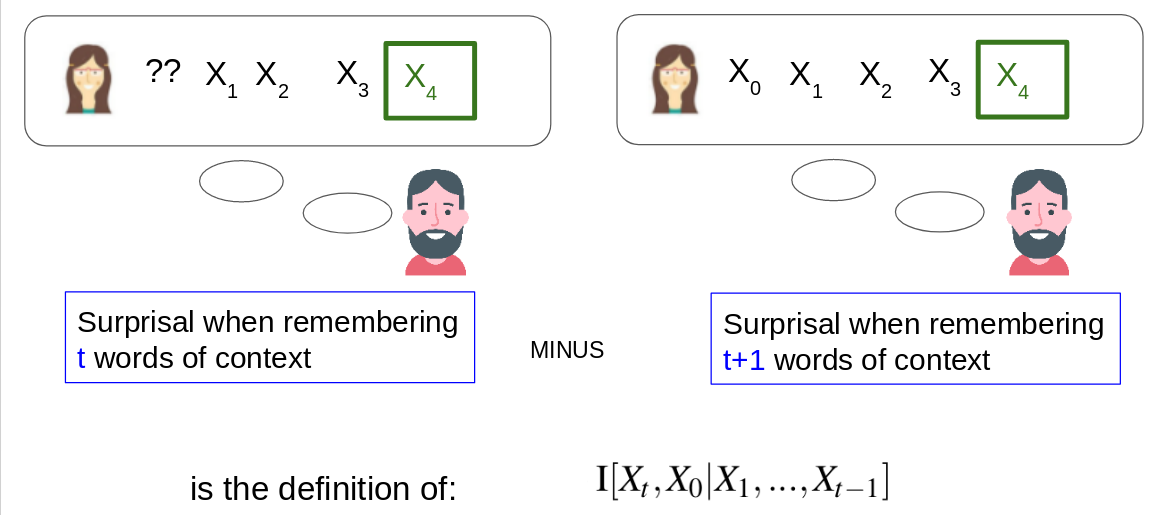
\includegraphics[width=0.9\textwidth]{figures/listener-it.png}
	\caption{(TODO adapt to format) Intuitive explanation of $I_t$}
\end{figure*}








We will use the concept of \emph{conditional mutual information}.
For two random variables $X, Y$, the mutual information $I[X,Y]$ is the reduction in entropy about $X$ by knowing $Y$:
\begin{equation}
	I[X,Y] := H[X] - H[X|Y]
\end{equation}
For three random variables $X, Y, Z$, the mutual information between $X$ and $Y$, conditional on $Z$, is this entropy reduction when $Z$ is already known:
\begin{equation}
I[X,Y|Z] := H[X|Z] - H[X|Z,Y]
\end{equation}
We will use the specific form where $X$ and $Y$ are observations $X_0$, $X_t$ of the process $(X_t)_{t \in \mathbb{Z}}$, and $Z$ is a block of intervening observations $X_1, \dots, X_{t-1}$:
\begin{equation}
	I[X_t, X_0 | X_1, \dots, X_{t-1}] := H[X_t| X_1, \dots, X_{t-1}] - H[X_t| X_0, X_1, \dots, X_{t-1}]
\end{equation}
This is equal to the reduction in uncertainty about the $t$-th observation when knowing the $0$-th observation, in addition to the block of intervening observations.
That is, we measure the amount of statistical dependency of observations that are $t$ steps apart, controlling for any information that is redundant with intervening observations.
This quantifies how much information needs to be carried across $t$ timesteps without any possibility for `guessing' it from intervening observations.



Using this concept, we can now state our first main result, concerning the memory load of a speaker: %, and of a listener performing optimal incremental prediction:

\begin{proposition}\label{prop:lower-bound}
	A speaker producing samples from $(X_t)_{t \in \mathbb{Z}}$ needs to maintain at least
\begin{equation}\label{eq:memory-bound}
M := \sum_{t=1}^\infty\ t \cdot \operatorname{I}[X_t, X_0 | X_1, ..., X_{t-1}]
\end{equation}
bits of memory on average.

\end{proposition}


Also can relax this to imprecise production: A speaker with low memory must deviate strongly from the language, measured in KL divergence.

%that the model does not have an `absolute clock' built into it.
The quantity $M$ is equal to the mutual information between past and future observations, $I[(X_i)_{i>0}, (X_i)_{i \leq 0}]$, which is often referred to as the \emph{excess entropy} of the process (CITE).




Due to the factor $t$ inside each term of the sum, carrying the same amount of information over longer distances requires more memory -- that is, modeling long statistical dependencies is more costly in terms of memory than modeling shorter ones.
This formalizes a general, assumption-free, link between memory and locality in language production.
In Section~\ref{sec:listener}, we will extend this analysis to listeners performing incremental prediction.
%incremental prediction.


The result in (\ref{eq:memory-bound}) is entirely information-theoretic and applies to \emph{any} physical encoding of the past, entirely independent of the implementation of the model. % and the mechanisms by which it computes predictions.
In particular, while the relation to psycholinguistic and psychological models of how memory works will be interesting to explore, our result applies to any such model.
Memory representations do not have to be rational or optimal for this bound to hold:
It provides a \emph{lower bound} on the amount of information that needs to be stored -- other memory representations will always need to store at least as much information.

We will write $I_t$ as an abbreviation for $\operatorname{I}[X_t, X_0 | X_1, ..., X_{t-1}]$.
The proposition implies that memory is decreased if $I_t$ decreases quickly as $t \rightarrow \infty$ -- that is, if the contributions of long-term dependencies in the process are small.
In particular, memory load can only be finite if $I_t$ decreases fast enough for the infinite sum to converge to a finite value.
%This confirms the intuition that finiteness of memory entails that the contribution of long-term 

We have treated the process $(X_t)_t$ as a discrete-time process whose time steps correspond to words, but this is immaterial to the analysis.
The analysis is not even restricted to discrete timesteps: We can replace the sum in~(\ref{eq:memory-bound}) with an integral to get a continuous-time version.



We illustrate Proposition~\ref{prop:lower-bound} in Figure~\ref{fig:basic}.
We consider two processes A and B, where $I_t := 5t^{-1.5}$ for $A$ and $I_t := 3.5 t^{-2.5}$ for $B$.
The curves of $I_t$, as a function of the distance $t$, are shown in Figure~\ref{fig:basic} (left).
In both cases, $I_t$ converges to zero as $t$ grows to infinity. 
However, $I_t$ decays more quickly for Process A (red).
This means that predictive information about an observation is concentrated more strongly in the recent past.
In Figure~\ref{fig:basic} (right), we show $t\cdot I_t$ as a function of $t$.
Note that the area under the curve is equal to (\ref{eq:memory-bound}).
This area is smaller for the red process, as $I_t$ decays more quickly there.  


\begin{figure*}
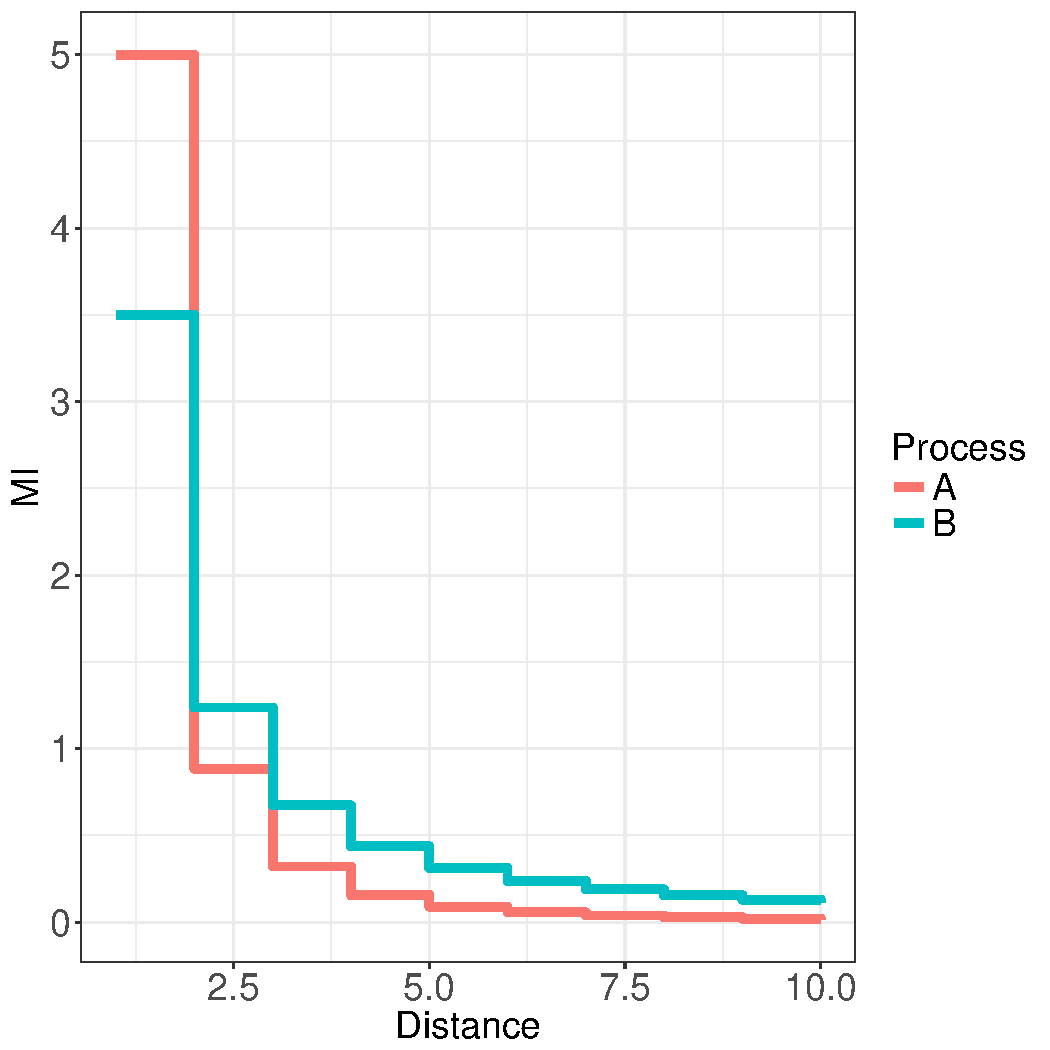
\includegraphics[width=0.45\textwidth]{toy/decay.pdf}
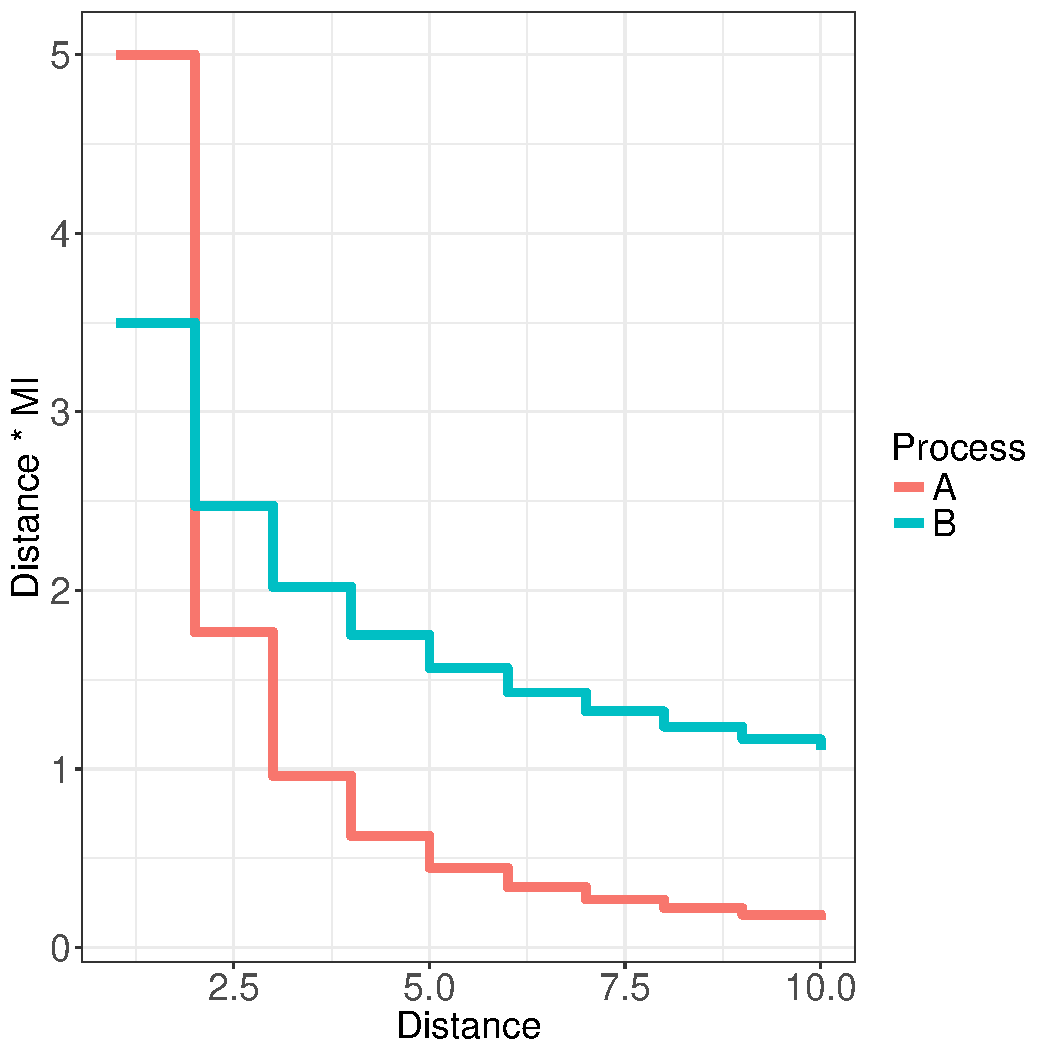
\includegraphics[width=0.45\textwidth]{toy/memory.pdf}
%
	\caption{Left: $I_t$ as a function of $t$, for two different processes. $I_t$ decays faster for the red process: Predictive information about the present observation is concentrated more strongly in the recent past. Left: $t \cdot I_t$ as a function of $t$ for the same processes. The area under the curves is given by (\ref{eq:memory-bound}). This area is smaller for the red process, as $I_t$ decays more quickly there.   }\label{fig:basic}
\end{figure*}


\subsection{Memory and Dependency Length}




We illustrate the linguistic predictions of Proposition \ref{prop:lower-bound} by reanalyzing the data from \cite{fedzechkina-human-2017}.
This is a miniature artificial language study that showed a bias for Dependency Length Minimization in production in artificial language learning.
Due to the controlled setting, it is possible to exactly compute the speaker's memory as given in~(\ref{eq:memory-bound}).


As ~(\ref{eq:memory-bound}) is invariant under reversal of the language, we only consider the head-final version of her artificial language.
The language has consistent head-final order, and uses case marking on objects.
The relevant production targets are transitive sentences where one of the two arguments is much longer than the other, due to the presence of a PP modifier, as shown in Table~\ref{tab:artificial}.
The language has variable order of subjects and objects; for the production targets, the B versions produce much longer dependencies than the A versions.
Dependency Length Minimization thus predicts that speakers are more likely to use the A versions.
\cite{fedzechkina-human-2017} confirmed this experimentally.


\begin{table}
	\textbf{A Orders: Short Dependencies}

		\begin{tabular}{ccc}
			Object & Subject & Verb \\
			\fbox{\begin{tabular}{llllll}
				\fbox{\begin{tabular}{llll} Adjective &Noun &Postposition\end{tabular}} & Noun-Case
					\end{tabular}} & \fbox{\begin{tabular}{l}Noun\end{tabular}} & \fbox{\begin{tabular}{l}Verb\end{tabular}}  \\
		\end{tabular}
\\
		\begin{tabular}{ccc}
			Subject & Object & Verb \\
			\fbox{\begin{tabular}{llllll}
				\fbox{\begin{tabular}{llll} Adjective &Noun &Postposition\end{tabular}} & Noun
					\end{tabular}} & \fbox{\begin{tabular}{l}Noun-Case\end{tabular}} & Verb \\
		\end{tabular}
\\
\\

	\textbf{B Orders: Long Dependencies}


		\begin{tabular}{ccc}
			Subject & Object & Verb \\
			 \fbox{\begin{tabular}{l}Noun\end{tabular}} &  \fbox{\begin{tabular}{llllll}
				\fbox{\begin{tabular}{llll} Adjective &Noun &Postposition\end{tabular}} & Noun-Case
		\end{tabular}}  &  \fbox{\begin{tabular}{l}Verb\end{tabular}}  \\
		\end{tabular}
\\
		\begin{tabular}{ccc}
			Object & Subject & Verb \\
			\fbox{\begin{tabular}{l}Noun-Case\end{tabular}} & \fbox{\begin{tabular}{llllll}
				\fbox{\begin{tabular}{llll} Adjective &Noun &Postposition\end{tabular}} & Noun
		\end{tabular}} & Verb \\
		\end{tabular}

			\caption{Production targets in the artificial mini language from \cite{fedzechkina-human-2017}. The language has head-final order, with free variation between SO and OS orders. When one of the arguments is much longer than the other, placing the longer one first (`A' orders) shortens syntactic dependencies, compared to `B' orders.}\label{tab:artificial}

\end{table}

In this section, we show that our bound on speaker memory makes the same prediction, without reference to syntactic structure or specific memory architectures. 

We constructed one language consisting of the A versions, and one language consisting of the B versions.
Following the experimental setup of \cite{fedzechkina-human-2017}, we assigned equal probability to the two possible configurations per language, and used a separate set of nouns (inanimate nouns) for the embedded noun in the long phrase.

We interpreted each of the two languages as a stationary processes, extending infinitely in both directions, by concatenating independent samples drawn from the language.
			We computed (\ref{eq:memory-bound}) from a chain of 1000 independently sampled sentences, for each of the two versions of the toy language.
			Figure~\ref{fig:toy-mis} (left) shows the curve of the conditional mutual information $I_t$ as a function of the distance $t$.
			The curves differ at $t=2$ and $t=5$: 
			About 0.073 nats of predictive information that are at distance $t=2$ in the A orders are moved to $t=5$ in the B orders.
%			In this sense, A orders have greater information locality than the B orders.
			%What is responsible for this difference?
			The source of the difference lies in predicting the presence and absence of a case marker on the second argument -- i.e., whether to anticipate a subject or object.
			In the A orders, considering the last two words is sufficient to make this decision.
			In the B orders, it is necessary to consider the word before the long second constituent, which is five words in the past.

			The total amounts of predictive information -- corresponding to the area under the curve -- are the same, indicating that both languages are equally predictable.
			However, we will see that the memory demands are different:
			Figure~\ref{fig:toy-mis} (right) shows $t\cdot I_t$ as a function of $t$.
			As $I_t$ decays faster in A orders, the total area under the curve now differs between A and B, and is larger in B.
			This area corresponds to the lower bound in (\ref{eq:memory-bound}), and is 2.21 nats in A orders, and 2.43 nats in B orders.
			While (\ref{eq:memory-bound}) is a general lower bound, it can be proven that this bound is actually tight in the case of this specific example.\footnote{This can be shown by computing the causal states and then showing that the crypticity is zero, both of which is tractable in the case of this small-scale artificial language.}
That is, a speaker who optimally allocates memory resources will spend 2.21 nats in A orders, and 2.43 nats in B orders.
It is important to stress that, even though we computed this value by considering the number of words impacting predictions at a given point in time, this bound holds independently of the actual implementation and architecture of memory and predictions.


\begin{figure*}
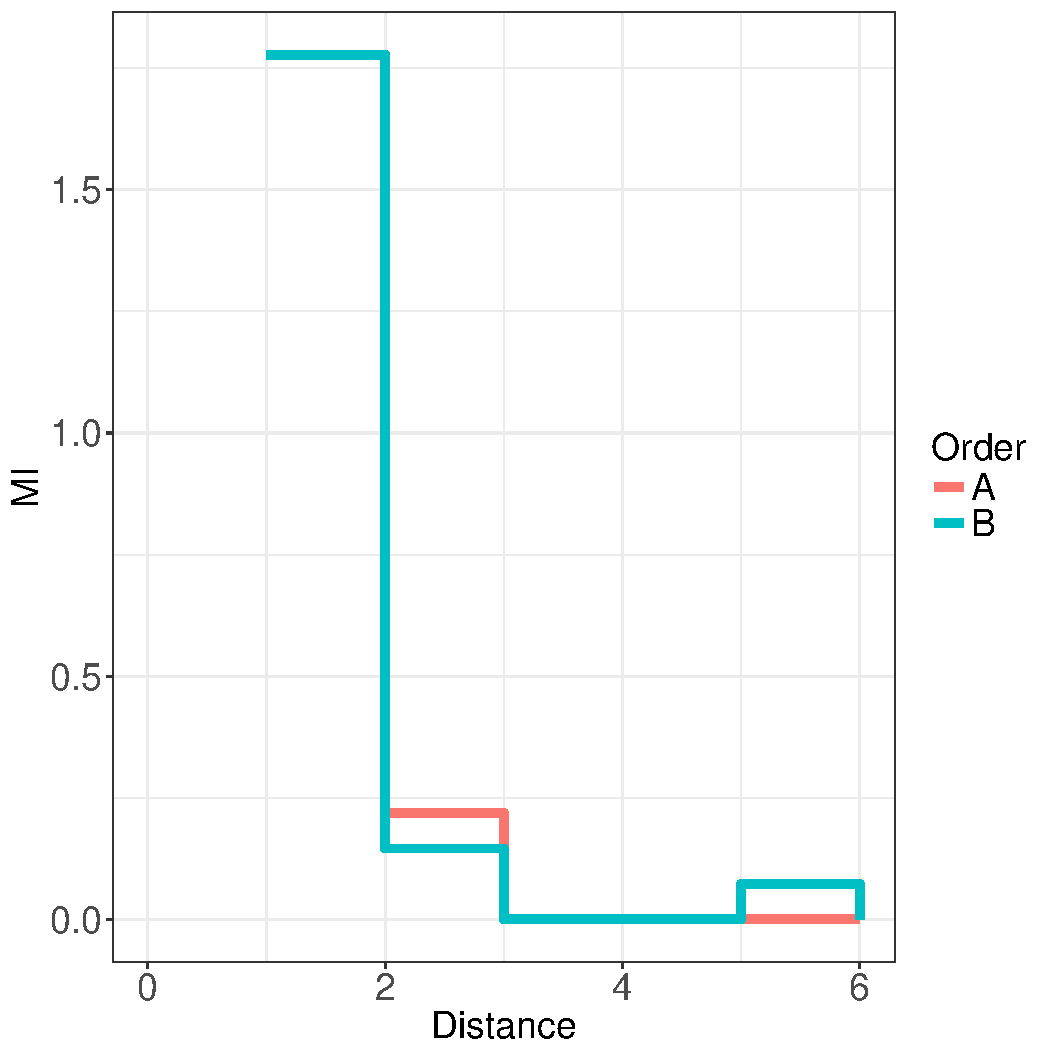
\includegraphics[width=0.45\textwidth]{toy/toy-mis.pdf}
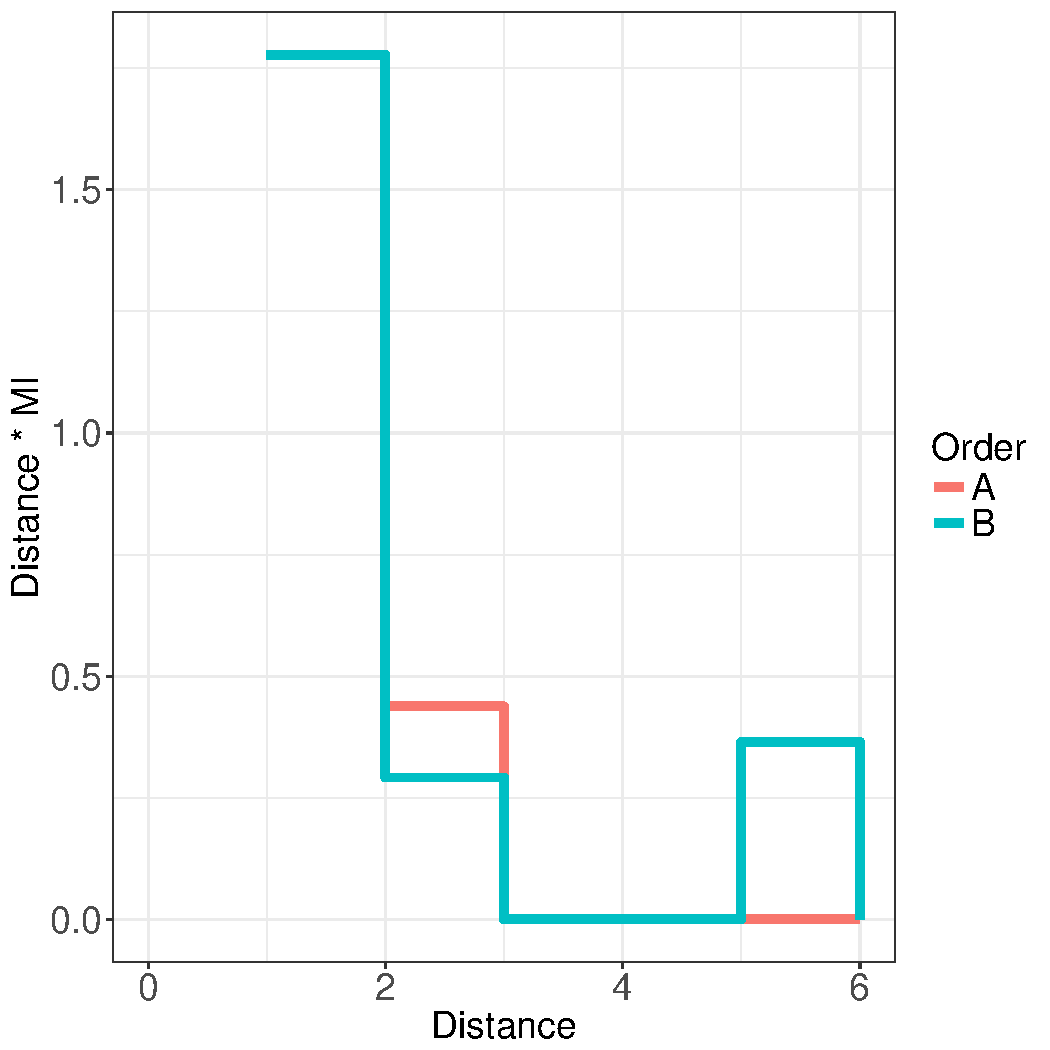
\includegraphics[width=0.45\textwidth]{toy/toy-t-mis.pdf}
%
	\caption{Left: Decay of Conditional Mutual Information, as a function of the distance $t$, for the two versions in the artificial language. The areas under the two curves are identical, corresponding to the fact that both orders are equally predictable. However, mutual Information decays faster in Order A.\ \ \ Right: $t I_t$, as a function of $t$. The area under the B curve is larger, corresponding to larger memory demand for this order.}\label{fig:toy-mis}
\end{figure*}
%Both languages have the same overall entropy rate, but they differ in the distribution of predictive information.
%
%plot of $I_t$
%
%The areas under the curves are identical.
%
%good version
%
%%CONTEXT LENGTH 0   2.06856758681  9997.93143241   0.0
%%CONTEXT LENGTH 1   0.29195106479  1.77661652202   1.77661652202
%%CONTEXT LENGTH 2   0.0729865489103  0.21896451588   2.21454555377
%%CONTEXT LENGTH 3   0.0729865489103  0.0   2.21454555377
%%CONTEXT LENGTH 4   0.0729865489103  0.0   2.21454555377
%%CONTEXT LENGTH 5   0.0729865489103  0.0   2.21454555377
%%CONTEXT LENGTH 6   0.0729865489103  0.0   2.21454555377
%
%bad version
%
%%CONTEXT LENGTH 0   2.06937301571  9997.93062698   0.0
%%CONTEXT LENGTH 1   0.291673373027  1.77769964269   1.77769964269
%%CONTEXT LENGTH 2   0.145830550934  0.145842822093   2.06938528687
%%CONTEXT LENGTH 3   0.145830550934  0.0   2.06938528687
%%CONTEXT LENGTH 4   0.145830550934  0.0   2.06938528687
%%CONTEXT LENGTH 5   0.0729152754672  0.0729152754672   2.43396166421
%%CONTEXT LENGTH 6   0.0729152754672  0.0   2.43396166421
%%CONTEXT LENGTH 7   0.0729152754672  0.0   2.43396166421
%%
%
%
%
%%
%%grammar:
%%
%%S $\rightarrow$ Obj Subj V (1/2) | Subj Obj V (1/2)
%%
%%Obj $\rightarrow$ NP di
%%
%%Subj $\rightarrow$ NP
%%
%%NP $\rightarrow$ N (3/4) | PP NP (1/8) | Adj NP (1/8)
%%
%%PP $\rightarrow$ NP P
%%
%
%





\subsection{Languages can trade off Memory Load and Predictability}
%\subsection{Speakers can can minimize Memory Load at Fixed Information Rate}

We have derived a general lower bound on the memory load of a speaker in Proposition~\ref{prop:lower-bound}.
We now relate the speaker's memory to the surprisal experienced by the listener.

The average surprisal of a language $(X_t)_{t \in \mathbb{Z}}$, as experienced by a listener performing optimal prediction, is equal to the entropy rate $H[X_t|X_{<t}]$.
This can be written as the unigram entropy minus the mutual information between a single observation $X_t$ and the past:
\begin{equation}
	H[X_t|X_{<t}] = H[X_t] - I[X_t, X_{<t}]
\end{equation}
where the unigram entropy $H[X_t]$ only depends on the frequencies of individual words, independently of the language's word order.

We will refer to the mutual information $I[X_t, X_{<t}]$ as the \emph{predictability} of the process.
The predictability $P := I[X_t, X_{<t}]$ is a lower bound on $M = I[X_{\geq t}, X_{<t}]$, and thus on speaker memory:
\begin{equation}
P \leq M
\end{equation}
and thus\footnote{More generally 
$H[X_t|X_{<t}] \geq \frac{1}{T} \left(H[X_{1\dots T}] - M\right)$ for any $T$. Thus, the following relation holds for any $T$: $$T \cdot \text{ListenerSurprisal} \geq H[X_{1\dots T}] - \text{SpeakerMemory}$$}
\begin{equation}
	Listener\ Surprisal \geq	H[X_t|X_{<t}] \geq H[X_t] - M \geq H[X_t] - Speaker\ Memory
\end{equation}
This means that, when we consider different languages that share a single unigram distribution, memory and surprisal trade off:
Languages that are highly predictable  require a good amount of speaker memory; a language that can be produced with very small memory cannot be very predictable.
In particular, a language that requires zero speaker memory must have zero predictability and maximal average surprisal.

We thus obtain a tradeoff between two different types of costs facing speakers and listeners: The \emph{speaker's} memory trades off with the \emph{listeners'} surprisal.



We can visualize this by placing languages into a \emph{memory-surprisal-plane} (Figure~\ref{fig:toy-mis}). Each language is assigned its entropy rate as its $y$ coordinate, and the memory load necessary to achieve optimal surprisal as its $x$ coordinate.
We will continue to assume that all languages share a single unigram distribution -- this will in particular apply when studying different word order variations of the same language.

The plane can be separated into an \emph{achievable} region, populated by languages, and an \emph{unachievable} region in which no languages can occur.
No language can have zero surprisal with zero memory -- the corner of the plane thus must fall in the unachievable region.
The boundary between the two regions is the \emph{Pareto frontier}.
Languages that fall on the boundary optimally trade off surprisal and memory; they cannot further decrease one without increasing the other.
The smallest possible values for this boundary consist of the points satisfying $P=M$, indicated by a straight diagonal line in Figure~\ref{fig:toy-mis}.
Only part of the achievable region will be populated by languages that could plausibly be natural languages: For instance, we may expect natural languages to have long-term dependencies that will prevent them from being at the absolute Pareto frontier.
We hypothesize that, if languages optimize the tradeoff between memory and surprisal, they will be close to the optimal boundary of a region populated by a `comparison class' of languages that share essential characteristics of natural language, but have other word order rules.
%When We will specify a class of baseline languages that we will argue to form a reasonable comparison class for natural language.
%Within this, we hypothesize that natural language is close to the Pareto frontier.


\begin{figure}
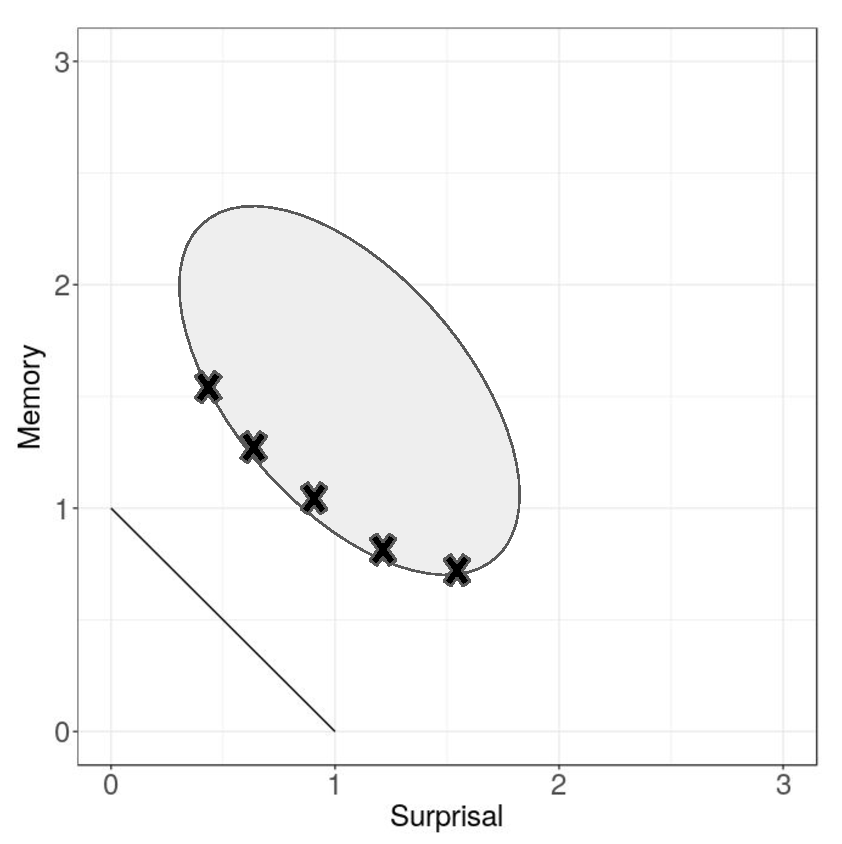
\includegraphics[width=0.45\textwidth]{toy/pareto-scheme.pdf}
%
	\caption{Memory-Surprisal Tradeoff. The straight line represents the Pareto frontier for unconstrained languages. Languages resembling natural languages inhabit a subset of the achievable region (grey oval). Its lower-left boundary represents the Pareto frontier relevant for natural language. We hypothesize that natural language lies close to this frontier.   }\label{fig:toy-mis}
\end{figure}



\subsection{Listeners can trade off Memory Load and Surprisal}\label{sec:listener}

%TODO redo curves so that x-axis is surprisal, y-axis the necessary memory

We have analyzed the memory load of a speaker and related it to the listener's surprisal.
We now analyze memory from the perspective of the listener, who needs to maintain information about the past to predict the future.
Similar to the listener maintains a memory state $L_t$; again, there are no assumptions about the memory architecture and the nature of its computations.
%We assume that the listener has no access to the speaker's state beyond what the speaker has already uttered.
We only make two basic assumptions about the flow of information:

First, we assume that the listener's internal state cannot depend on the future beyond its dependency on the past.
Formally: 
\begin{equation}\label{eq:listener-markov-1}
L_t \bot X_{>t} | X_{\leq t}
\end{equation}
This means that the listener has no access to the speaker's state beyond what the speaker has already uttered.

Second, we assume that $L_t$ contains no information about the past beyond what is contained in $X_{t-1}$ and $L_{t-1}$:
\begin{equation}\label{eq:listener-markov-2}
L_t \bot X_{<t} | X_{t-1}, L_{t-1}
\end{equation}
This means that any information about the past in $L_t$ has to be contained in $L_{t-1}$ -- formalizing the idea that a listener can only remember aspects of the past by keeping them in memory, and that memories of the past cannot `spontaneously' form later in the future.

The listener can trade off memory and future surprisal:
A listener who chooses to store less memory will exerience higher surprisal in the future.
A listener can achieve minimal surprisal -- that is, the lowest average surprisal that any model could achieve by predicting the future from the past -- if and only if $L_t$ contains all predictive information about the future that is contained in the past.

We will describe this tradeoff, and show that listener memory is linked to locality in a way similar to speaker memory.
Consider a listener who uses $J$ bits of memory on average.
What can we say about the listener's surprisal?
We return to the information and memory curves in Figure~\ref{fig:basic}.
In the graph of $t \cdot I_t$, we look for the first $T$ such that the area under the curve to the left of $T$ has size $\geq J$.
This is illustrated in Figure~\ref{fig:listener-tradeoff-decay} (right).
Then let $\epsilon$ be the area under the curve of $I_t$ to the right of $T$ (Figure~\ref{fig:listener-tradeoff-decay}, left).
We can prove that such a listener must incur surprisal at least $\epsilon$ greater than a listener with perfect memory.
As before, we write $$I_t := I[X_t, X_0 | X_{1\dots t-1}]$$
Then


\begin{proposition}\label{prop:suboptimal}
	Let $T$ be a positive integer, and consider a listener using at most
$$\sum_{t=1}^T t I_t$$
bits of memory on average.
Then this listener will incur surprisal at least
	$$H[X_t|X_{<t}] + \sum_{t > T} I_t$$
	on average.
\end{proposition}


The proposition gives us a lower bound on the listener's memory-surprisal curve: Taking all pairs of memory $\sum_{t=1}^T t I_t$ and surprisal $H[X_t|X_{<t}] + \sum_{t > T} I_t$, we obtain a curve in memry-surprisal plane, which is a lower bound on the memory demands of any listener at a given surprisal level.
We visualize this for the two processes from Figure~\ref{fig:basic} in Figure~\ref{fig:listener-tradeoff}.

\begin{figure}
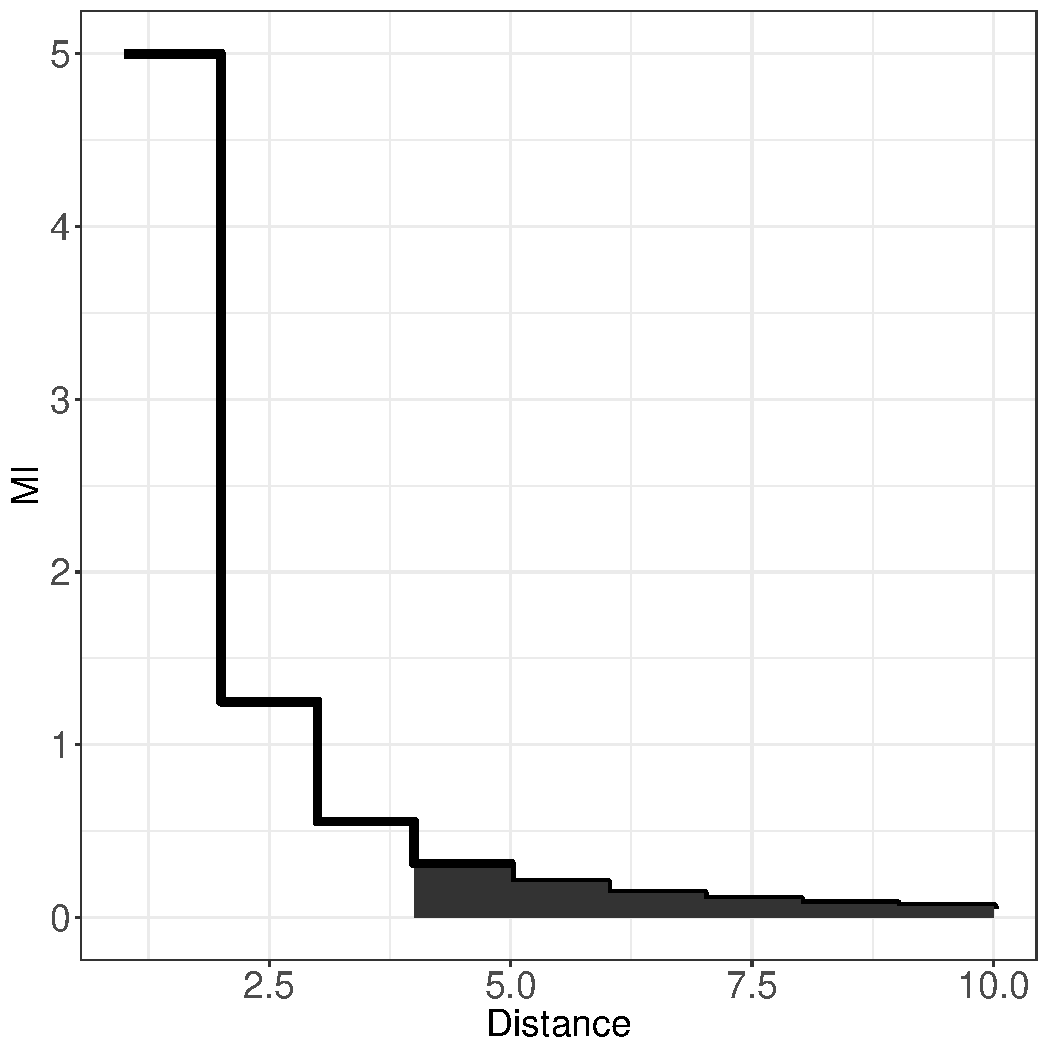
\includegraphics[width=0.45\textwidth]{toy/add-surp.pdf}
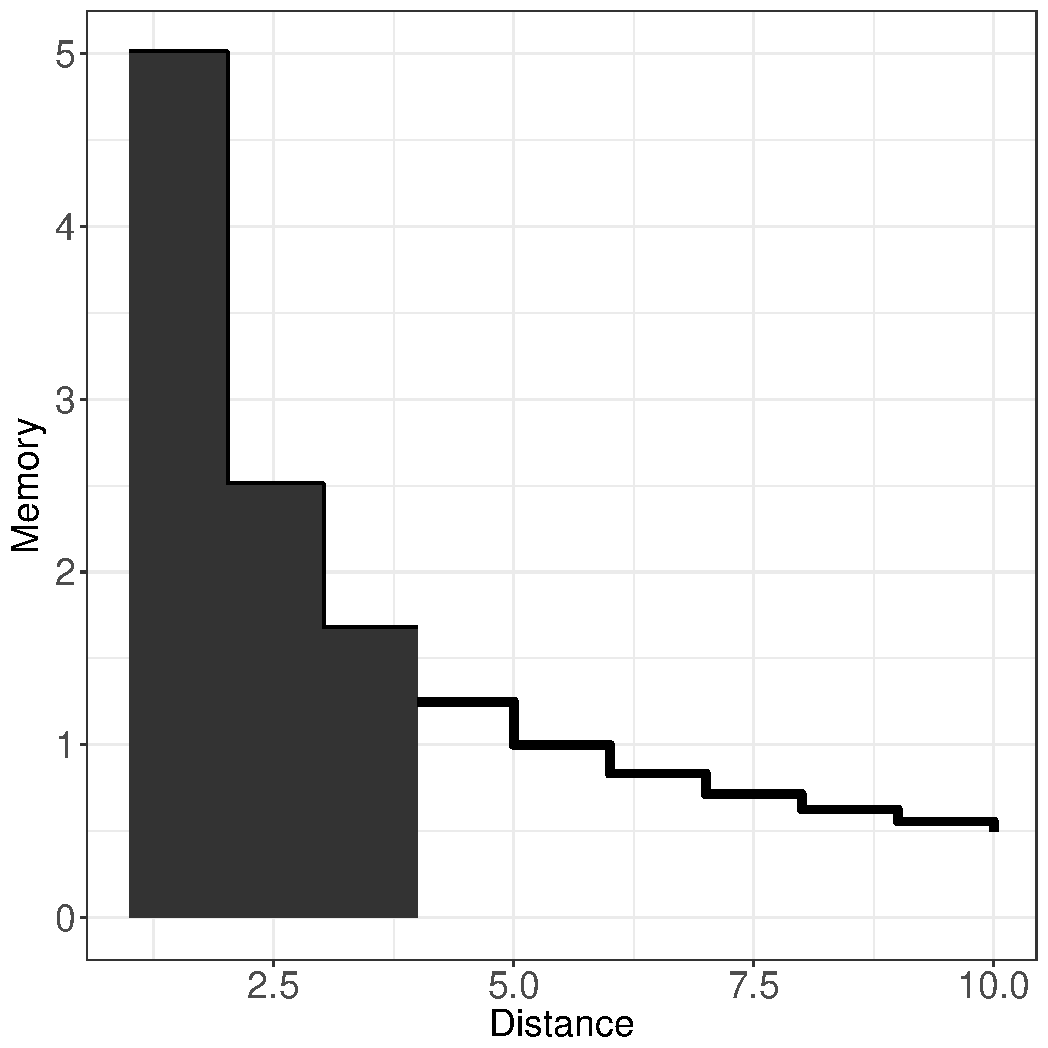
\includegraphics[width=0.45\textwidth]{toy/lower-mem.pdf}
	\caption{Illustration for Proposition~\ref{prop:suboptimal}. Listeners can trade off memory and surprisal: A listener only investing memory of the amount given by the black area on the right will incur at least the black area on the left in additional surprisal. In the given example, $T=4$. By varying $T$, the two areas describe the listener's memory-surprisal tradeoff curve.}\label{fig:listener-tradeoff-decay}
\end{figure}




\begin{figure}
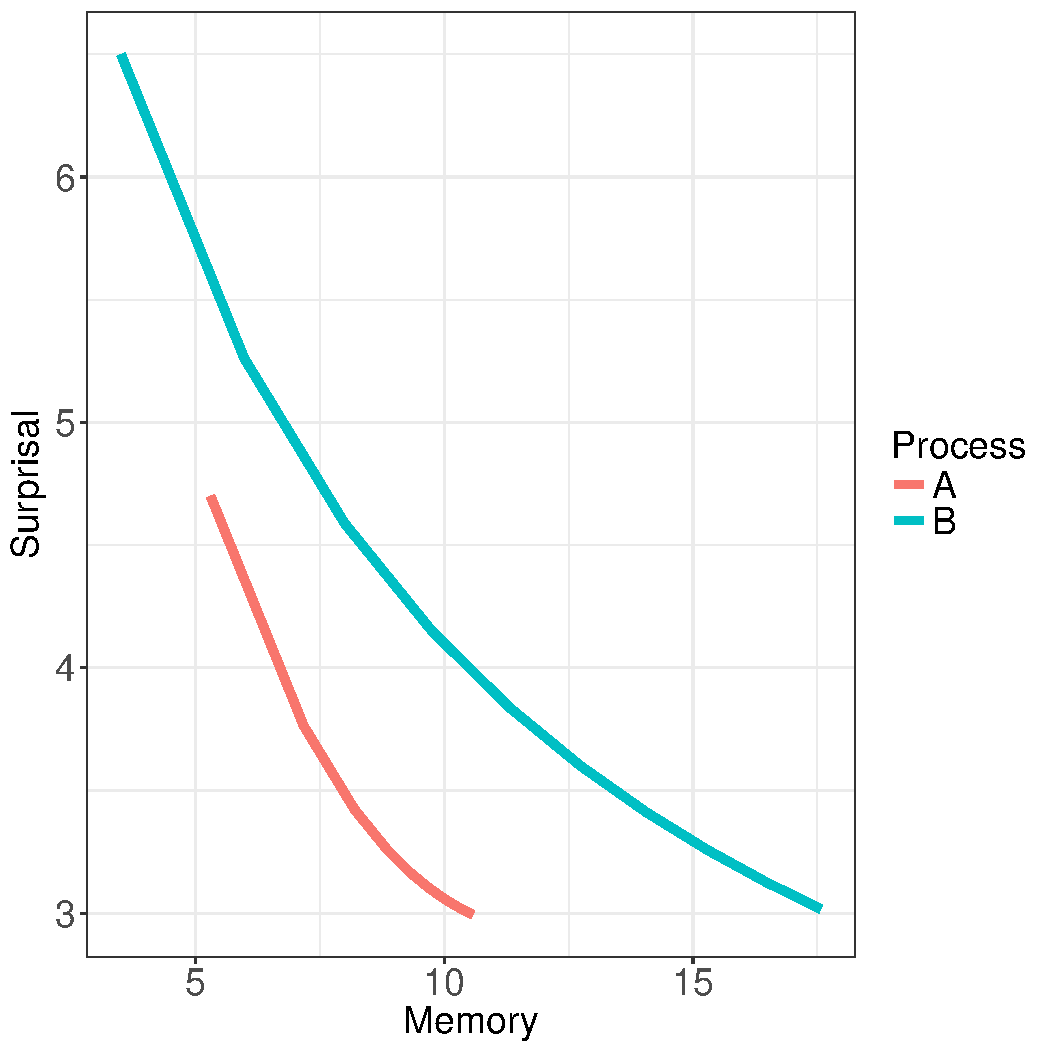
\includegraphics[width=0.45\textwidth]{toy/listener-tradeoff.pdf}
	\caption{Listener's memory-surprisal tradeoff for the two processes in Figure~\ref{fig:basic}. Recall that the red process had a faster decay of conditional mutual information. Correspondingly, this figure shows that a listener can achieve lower surprisal at the same level of memory load.}\label{fig:listener-tradeoff}
\end{figure}


In Figure~\ref{fig:toy-listener-tradeoff}, we show the resulting curve for the two versions of the artificial language from \cite{fedzechkina-human-2017}.
In this language, speaker memory coincides with the memory demand of a listener who performs optimally in incremental prediction.
The curve shows that, at any desired level of surprisal, Order A requires at most as much memory as Order B.
For reaching optimal surprisal, Order A requires strictly less memory.
Thus, in this case, the listener's surprisal-memory tradeoff is optimized by the orders predicted by Dependency Length Minimization.

\begin{figure}
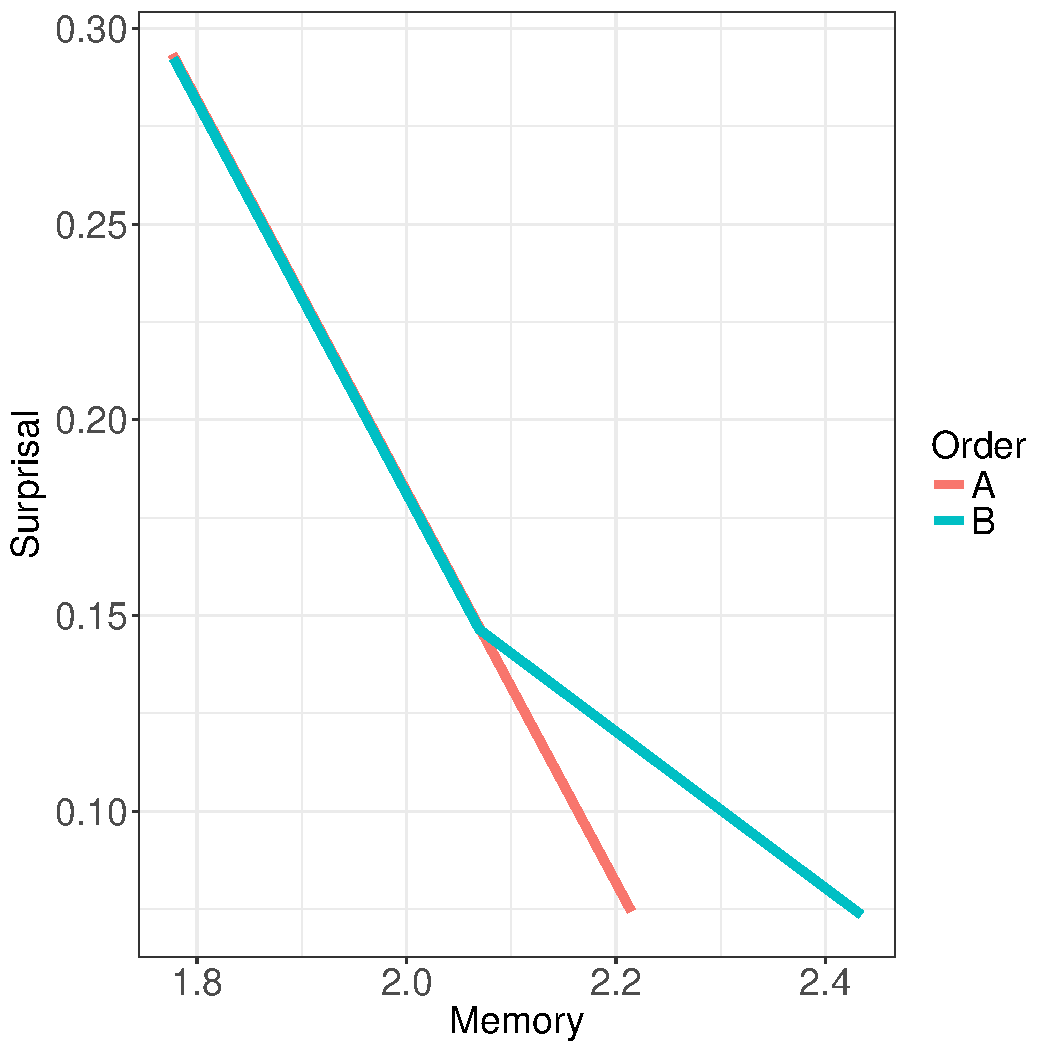
\includegraphics[width=0.45\textwidth]{toy/toy-mem-surp.pdf}
	\caption{Tradeoff between listener memory and surprisal, for the two versions of the artificial language from \cite{fedzechkina-human-2017}. Language A requires less memory at the same level of surprisal.}\label{fig:toy-listener-tradeoff}
\end{figure}


\paragraph{Center Embeddings}

\cite{miller-finitary-1963} attributed the unacceptability of multiple center-embedding to memory limitations.


%\cite{gibson-linguistic-1998}

%first center-embeddings, POS level model

%Later work found evidence that cross-serial dependencies are less taxing.


%now cross-serial: POS level model things are the same. But lexical level, assume PMI and dependencies. Then listener's tradeoff is better for cross-serial dependencies


\subsection{Relation to Theories of Sentence Processing}


\paragraph{Lossy-Context Surprisal}
\citet{futrell-noisy-context-2017} describe a processing model where listeners make predictions (and incur surprisal) based on lossy memory representations.
In particular, they consider loss models that delete, erase, or replace words in the past.
Under the assumption that loss affects words more strongly that are further in the past, they derive a principle of information locality:
A listener will incur surprisal
$$ -\log P(w_t) - \sum_{j=1}^{t-1} f(i-j) pmi(w_i; w_j) + R$$
where the `survival probability' $f(d)$ decreases as the distance $d$ between two words increases, and $R$ is a remainder term that can be argued to be small.
Given that $f$ is assumed to be decreasing, this prediction loss will be smaller when words with high mutual information are closer together in the input.
Our Proposition~\ref{prop:suboptimal} can be seen as an analogous result for general models of memory.






\paragraph{Relation to Dependency Locality}
The quantity described in Proposition~\ref{prop:lower-bound} is formally similar to Storage Cost in the Dependency Locality Theory (DLT) \citep{gibson-linguistic-1998}: Storage cost at a given timestep is defined as the number of predictions that are held in memory.
Storage cost only considers predictions that are certain, and each prediction takes an equal amount of memory.
In contrast, the result in Proposition~\ref{prop:lower-bound} can be seen as weighting predictions by their certainty and the amount of predictive information.
In this sense, DLT storage cost can be seen as an approximation to Proposition~\ref{prop:lower-bound}.



\paragraph{Center Embeddings, ...}
Yngve 1960, had a complexity measure, but doesn't work well for left-branching structures

Miller and Chomsky 1963

Frzier 1985 local nonterminal count

Rambow and Joshi 1994 using TAG

Marcus 1980 deterministic parsing

(Sabrina Gerth, Memory Limitations in Sentence Processing)


\subsection{Relation to other work}

\paragraph{Statistical Complexity}
There are deep connections between our formalization of speaker and listener memory and studies of dynamic systems in the Physics literature.
Our formalization of listener memory, under the assumption of optimal prediction, is equivalent to the notion of \emph{Statistical Complexity} \citep{crutchfield-inferring-1989}.
Speaker memory corresponds to \emph{Generative Complexity} \cite{loehr-non-sufficient-2008, loehr-predictive-2010}.
The tradeoff between listener memory and surprisal is formally equivalent to the \emph{Recursive Information Bottleneck} considered by \cite{still-information-2014}.
The quantity in (\ref{eq:memory-bound}) is equal to the \emph{excess entropy}, and it has long been known to bound statistical and generative complexity \citep{crutchfield-inferring-1989}.
However, the link between memory and locality provided by our series expansion in (\ref{eq:memory-bound}) appears to be a novel contribution.


\cite{sharan-prediction-2016} shows a link between excess entropy and approximability by $n$-th order Markov models, noting that processes with low excess entropy can be approximated well with Markov models of low order.



\paragraph{Decay of Mutual Information}
In Propositions~\ref{prop:lower-bound} and \ref{prop:suboptimal}, we showed a close link between memory and the decay of \emph{conditional} mutual information $I_t := I[X_t, X_0 | X_{1\dots t-1}]$.
Prior work has studied the decay of \emph{unconditional} mutual information $I[X_t, X_0]$ in natural language \citep{ebeling-entropy-1994,lin-critical-2017}, and linked it to locality and memory \citep{futrell-noisy-context-2017}.

The decay of unconditional mutual information is less closely linked to memory requirements than conditional mutual information:
While the decay of conditional mutual informations provides a lower bound on memory need, unconditional mutual information does not:
Consider the constant process where with probability 1/2 all $X_t = 0$, and with probability 1/2 all $X_t = 1$. %%$X_t = c$, where $c$ is random but independent of $t$ for each specific draw from the process.
The unconditional mutual information is 1 at all distances, so does not decay at all, but the process only requires 1 bit of memory.
Conversely, one can construct processes where the unconditional mutual informations are 0 for all $t$, but where $P > 0$ and this predictive information is actually spread out over arbitrarily large distances (that is, the ratio of memory $M$ and predictability $P$ can be made arbitrarrily large).\footnote{First, consider the process (called X by REF) consisting of 2 random bits and their XOR. This one has bounded nonzero $J$, but zero unconditional MI. To get unbounded $J$, consider the following process for any $N \in \mathbb{N}_{>2}$: Every $X_t$ is equal to the XOR of $X_{t-1}$ and $X_{t-N}$, such that each $X_t$ has $Bernoulli(1/2)$ as its marginal. The unconditional mutual information between any two timesteps is zero, but modeling the process requires $N$ bits of memory.}



\paragraph{Long-range dependencies in text}    % excess entropy
\cite{debowski-excess-2011} has studied the excess entropy of language across long ranges of text, in particular studying whether it is finite. % compute excess entropy in text
Our work contrasts with this work in that we are interested in dependencies within sentences.


\subsection{Discussion}

\paragraph{Speakers vs Listeners}
Our results apply both to speakers and listeners.

\paragraph{Decay vs Interference}
Work has suggested that interference and memory overload is more appropriate than decay \cite[p. 408]{lewis-activation-based-2005} for modeling locality and memory in sentence processing.
The bounds in Propositions~\ref{prop:lower-bound} and \ref{prop:suboptimal} hold for any type of memory model, and are thus compatible with decay- or interference-based models.
The formula in (\ref{eq:memory-bound}) might suggest that boundedness of memory entails that memory has to decay.
This is not the case:
A long dependency can be maintained perfectly with low average memory:
Informally, if every sentence is $N$ words long and has one long-distance dependency spanning the entire sentence, this dependency can be modeled perfectly with a memory cost that is independent of $N$.
In contrast, if every symbol strongly and non-redundantly depends on the character $T$ steps in the past, with $T$ large, this will create a memory cost proportional to $T$.




\paragraph{Memory and Hierarchical Structure; Finiteness of Memory}
Processing nontrivial hierarchical structures typically requires unbounded amounts of memory.
However, crucially, the \emph{average} memory demand for prediction can be finite, if the probability mass assigned to long dependencies is small.
In fact, languages defined by Probabilistic Context Free Grammars (PCFG) always have finite average memory (and thus in particular finite excess entropy):


\begin{proposition}
Any language generated by a PCFG, with rational weights, and finitely many terminals and nonterminals, has finite average memory demand in production and incremental prediction.
\end{proposition}

\begin{proof}[Proof Sketch]
	We provide an algorithm that performs generation or optimal prediction and has finite average memory use. We consider incremental Earley parsing \citep{earley-efficient-1970}. Disregarding probabilities, parsing a word of length $n$ takes $O(n^2)$ bits of memory (where the constants depend on the grammar but not $n$). For storing probabilities, the storage will be similarly bounded as long as the weights of the grammar are rational.
	The result then follows from Proposition 2 in \cite{chi-statistical-1999}, which says that any function that is polynomial in the length of words drawn from a PCFG has finite expectation.\footnote{Using Proposition 2 of \cite{chi-statistical-1999}, one can also directly show that excess entropy is finite for any PCFG (without assumption about the weights), if we interpret it as giving rise to a stationary process consisting of a sequence of words independently drawn from the language.}
\end{proof}



\section{Heavy NP Shift}


Phenomenon linked to locality/memory (Hawkins)

Is the listener's memory-surprisal tradeoff optimized by Heavy NP Shift?

Penn Treebank

Trained 20 language models counterfactual version

then estimate memory on real and reverse orderings


3) Describe the key dependent variable(s) specifying how they will be measured.
Collect all instances of a VP consisting of a verb, and (in some order) an NP and a PP, from the Penn Treebank (WSJ) training set. Calculate the listener's memory-surprisal tradeoff on the words belonging to the NP and the PP.


5) Specify exactly which analyses you will conduct to examine the main question/hypothesis.
(1) Is the listener's memory-surprisal tradeoff significantly better on real as opposed to inverted order of the NPs and PPs? Is this separately true for cases where NP-PP is the real ordering, and for cases where it is PP-NP? This will be tested by bootstrapping over language models and examples.
(2) Is the listeners memory-surprisal tradeoff significantly better when placing the shorter constituent (of this NP and PP) before the longer one?
Also tested by bootstrapping over language models and examples.

6) Describe exactly how outliers will be defined and handled, and your precise rule(s) for excluding observations.
Language models with overall validation average surprisal > 10 will be excluded (this didn't happen).

7) How many observations will be collected or what will determine sample size?
20 LSTM language models are constructed on a version of Penn Treebank where for all verb-initial VPs, the order of the remaining daughter constituents is shuffled.


Is the listener's memory-surprisal tradeoff significantly better on real as opposed to inverted order of the NPs and PPs?

Is this separately true for cases where NP-PP is the real ordering, and for cases where it is PP-NP?

Is the listeners memory-surprisal tradeoff significantly better when placing the shorter constituent (of this NP and PP) before the longer one?

%
%
%\section{NP Structure}
%
%- adjective order
%
%- noted by ...: Det - Num - Adj
%
%
%This is a case where the predictions differ from DepL
%
%
%E.g., if the choice of determiners, numerals, and adjectives are statistically independent when conditioning on the noun, will predict the effect.
%Computationally verify the effect.


\section{Large-Scale Evidence that natural language optimize Memory-Surprisal Tradeoff}

We now investigate whether word orders as found in natural language optimize the two memory-surprisal tradeoffs.
We will define a class of baseline languages that serve as a comparison class of word orders that natural language can be compared to.

Ordering grammars are defined as in the Optimization paper: For each UD relation type, define a weight. To get random baseline languages, randomize the weights.
All grammars are valuated deterministically.

We found that, across treebanks, random grammars that have more fine-grained rules or are evaluated nondeterministically do worse in both memory-surprisal tradeoffs.
Thus, random grammars with by-relation weights constitute a stronger baseline.


%Things that one may ponder: (1) what are even stronger baselines? (2) probably should do a control experiment using maximum-likelihood fits


%\subsection{Prediction on the level of POS}
%As mutual information cannot be realiably estimated on many of the smaller corpora in the UD project, we first compute (\ref{eq:memory-bound}) on the level of POS tags -- that is, we compute memory need for incremental prediction of POS sequences. %, following~\cite{futrell-noisy-context-2017}.
%As the summation in~(\ref{eq:memory-bound}) terminates when $t$ is greater than the length of any sentence, we can compute this quantity exactly for the empirical distribution over sentences in a given corpus.
%
%%We computed these quantitities for the optimized languages, the original languages, and for baseline  languages. For each language, we created 50 baseline ordering models, for which $a_\tau, b_\tau$ where drawn uniformly from $[-1, 1]$.
%%As mutual information between words is decreased if the language exhibits additional randomness (as our stochastic ordering models do) -- which decreases memory demands but increases entropy -- we hold the entropy of our languages constant by replacing each sampling step with taking the maximum -- that is, we take the zero temperature limit.
%%This ensures that all versions of a given language have the same entropy, and makes the numbers for memory demand comparable.
%%
%%%\mhahn{TODO results across languages}
%%
%%%We find that, averaged across all 50 languages, optimized models require less memory than 93 \% of the respective baseline models.
%
%Results for four languages are shown in Figure~\ref{fig:memory-results}.
%Averaged across languages, natural language requires less memory than 87 \% of random baseline ordering models.
%%Languages which require less memory than all baseline languages had significantly lower word order freedom ($t = -4.061$, $p = 0.00018$).
%
%
%%%For half of the languages
%%For 75 \% of all languages, the LSTM-optimized version takes less memory than 95 \% of the baseline models.
%%For 37 \% of the languages, it also requires less memory than the original language.
%
%%We found that, as predicted, memory usage in real languages was correlated with word order freedom:
%
%
%%\begin{figure*}
%%\includegraphics[width=0.98\textwidth]{figures/memory-demand-upos-facets.pdf}
%%%
%%\caption{Memory demands of real, optimized (for ease of LSTM language modeling), and baseline versions of languages computed using~(\ref{eq:memory-bound}): Optimizing for ease of language modeling results in languages that require less memory in incremental prediction. On the level of POS tags, languages with fixed word order minimize memory need, while languages with very free word order, such as Basque, have similar memory requirements to baseline languages.}\label{fig:memory-results}
%%\end{figure*}
%%

\subsection{Method}
The small size of available syntactic data for many languages means that estimating mutual information is problematic.


In general, we expect a bias-variance tradeoff:

A method that estimates on a coarse-grained level (e.g. POS) will result in estimates with relatively higher fidelity and lower variance, potentially making it easier to localize the actual language in the space of counterfactual languages.
However, it introduces \emph{bias} by describing a simplified version of the language.





We propose to therefore compute the quantities on levels less likely to suffer from data sparseness: part-of-speech and morphology.

In the UD treebanks, each word has part-of-speech and morphological information.
The UD treebanks encode morphology by providing, for each word in a sentence, a sequence of feature-value pairs (e.g., NUMBER=Singular).
We encode each word into (1) its POS tag, (2) the sequence of these morphological feature-value pairs, (3) a special end-of-word token that indicates that information related to the word ends.
We further provide the word's lemma after its POS tag, if it is one of the 50 most frequent lemmas of the language.
Each POS tag and morphological feature-value pair is encoded as an atomic token.
The rationale for including frequent lemmas is that such words often are strongly grammaticalized and may provide grammatical information (and frequent words are less likely to be affected by data sparseness).


To estimate mutual informations, we use LSTM recurrent neural networks, the basis of the state of the art in modeling sequences such as natural language.
We will discuss alternative estimation methods below.

During incremental prediction, the LSTM sequentially reads these tokens and computes a distribution over the next word.
The probability that the LSTM assigns to a word -- encoded as a bundle of POS and morphological features -- in a context is the product of the contextual probabilities of the POS tag, the feature-value pairs, and the end-of-word token (the purpose of the end-of-word token is to make this possible -- we couldn't compute the probability of a word directly without this).


Given a corpus, we estimate a language model by training the LSTM on a training partition to maximize the data likelihood, and stopping training once the data likelihood on a held-out partition drops.
The hyperparameters (number of hidden units, learning rate, etc.) are chosen so as to maximize the likelihood of the held-out partition.
This procedure helps prevent overfitting the model to the training data, and ensure that it generalizes to unseen data. 

Note that the quantities $\operatorname{I}[X_t, X_0 | X_1, ..., X_{t-1}]$ in~(\ref{eq:memory-bound}) are equal to difference between conditional entropies $H[X_t|X_1, ..., X_{t-1}] - H[X_t|X_0, X_1, ..., X_{t-1}]$.
Therefore, to compute this quantity, we compute the differences between the surprisals
$-\log P[X_t | X_0, X_1, ..., X_{t-1}]$ and $-\log P[X_t | X_1, ..., X_{t-1}]$ for each word in the held-out partition, and take the average over these.
We cut $T$ off at 30.


\paragraph{Alternative Models}
Recent research has proven strong theoretical learnability guarantees for neural network models (CITE), supporting their success in practice.
They also provide the strongest predictors of the surprisal effect on human reading times \citep{frank-insensitivity-2011, goodkind-predictive-2018}.

In view of the NLP literature, the following are the main other options that exist for estimating mutual information and probabilities in sequences:

First, an n-gram model: Here, the problem is that n-grams do not express any morphosyntactic generalizations. Furthermore, standard n-gram models do not express any generalizations about pairs of words that are not adjacent -- e.g., encoding a generalization about morphological agreement between two words is hard for such a model to capture if the two words are not always adjacent. Both the small scale of available corpora in many languages and free word order in many languages with rich morphology thus seem to make such models unattractive.

A statistical grammar: It may sound natural to model morphosyntax with a hierarchical grammar. The challenge is to encode statistical morphosyntactic generalizations, and to decide which independence assumptions to put into the model. One can either decide on a language-specific basis which generalizations to put in (laborious and might introduce bias), or choose a general model family that is rich enough to learn generalizations. The second option will make this a machine learning model that, for our purposes, does not seem to be superior to a recurrent neural network.




\subsection{Data}
We considered all languages for which there are Universal Dependencies 2.2 treebanks with a total of at least 400 sentences of training data.
We excluded data from historical languages.\footnote{Ancient Greek, Coptic, Gothic, Latin, Old Church Slavonic, Old French.}
We excluded four languages for a later confirmatory experiment (English, Korean, Russian). % Irish
This resulted in X languages.

For most language, we used the predefined data split.
For some languages, where there was no training partition, or where the training partition was smaller than the test partition, we redefined the split to obtain more training data:
For these languages, we randomly pooled all the available partitions, used 100 sentences as held-out data, and used the remainder as training data.\footnote{This affects Amharic, Armenian, Breton, Buryat, Cantonese, Faroese, Kazakh, Kurmanji, Naija, Thai, and Uyghur.}

\subsection{Setup}
The recurrent neural network architecture has a range of adjustable parameters such as the number of neurons.
For each language, we used Bayesian optimization using the Expected Improvement acquisition function (CITE) \citep{snoek-practical-2012} to find a good setting of the hyperparameters, taking average surprisal on random grammars as the objective.
This biases the hyperparameters towards favoring counterfactual grammars.

This experiment is not fully confirmatory, since some data was collected for some languages before the predictions and the setup of the experiment were finalized.

For each language, we collected data from the actual orderings and from random grammars.
We collect multiple samples for the actual orderings to control for variation due to the random initialization of the neural network.
We collected data from the actual and random orderings in proportion one to three.
The stopping criterion will be described below.




\paragraph{Speaker Memory: Distance from Pareto Frontier}
We want to test: Are languages closer to the Pareto frontier than baseline languages tend to be?

For this, we need a way of quantifying distance to the Pareto frontier.
We suggest to measure the distance as the fraction of baseline languages that are better on both dimensions.

More formally, fixing a natural language, let $P_0$ be the distribution of baseline languages mapped to the surprisal-memory plane, viewed as a probability distribution over the positive quadrant of the plane $\mathbb{R}_+^2$.
For any point $x \in \mathbb{R}_+^2$, let $A_x$ be the fraction of baseline languages that are better on both dimensions.
Similarly, let $B_x$ be the fraction of baseline languages that are worse on both dimensions.
Using the probability distribution $P_0$, we can write:
$$A_x := P_0(\{X : X_1 \leq x_1 \wedge X_2 \leq x_2\})$$
$$B_x := P_0(\{X : X_1 \geq x_1 \wedge X_2 \geq x_2\})$$
%Ways of using this to test and quantify for distance (I think they are all reasonable and worth reporting in SI. Question is which ones to rely on mostly for the main part):
Futher, let $P_1$ be the distribution in the surprisal-memory plane that is generated by the results obtained for the real orderings, with different random initializations.
For each language, we \emph{test} the hypothesis that the language optimizes the tradeoff by considering the null hypothesis that the real orderings do not Pareto-dominate more baseline orderings than there are baseline orderings dominating them:
$$\E_{x \sim P_1} [B_x] \leq \E_{x \sim P_1}[A_x]$$

We propose to \emph{quantify} closeness to the frontier using the following two statistics:

\begin{enumerate}
%	\item CIs for $C_x := B_x - A_x$ may be a resonable stopping criterion
	\item  $E := \frac{\E_{x \sim P_1}[A_x]}{\E_{x \sim P_1}[A_x+B_x]}$

		This has the following interpretation: Among orderings that either dominate or are dominated by the real orderings, what fraction is dominated by the real orerings?
		This quantity is $1$ if the real orderings are not Pareto-dominated by any baseline order, but do dominate some baseline orders.
		The null hypothesis defined in our test amounts to the inequality $\E_{x \sim P_1}E_x \leq 0.5$.

A drawback of this quantity is that it is meaningless when the real orders do not dominate, and are not dominated by, any real order.
The following quantity is always maningful:

	\item Compute $A_{x'}$ for each $x'$ from the baseline distribution $P_0$, and then calculate the percentile rank of $\E_{x \sim P_1}[A_x]$ among these values:
		$$D := P_0(A_X \leq \E_{x \sim P_1}[A_x])$$
This statistic describes how many random orders achieve closer distance to the frontier as measured by $A_x$.
		Stated differently, it quantifies how `extraordinary' the value $\E_{x \sim P_1}[A_x]$ is in relation to values typically attained for $x' \sim P_0$.
The statistic is close to zero if $\E_{x \sim P_1}[A_x]$ is smaller than for almost all samples from $P_0$.

\end{enumerate}

We will obtain confidence intervals for the statistics via bootstrapping, and use a confidence interval for $B_x-A_x$ for testing $B_x \leq A_x$.
In the appendix, we report simulations that justify the use of bootstrapping in this situation.

\paragraph{Listener Memory: Surprisal-Memory Tradeoff}
We want to test whether languages' surprisal-memory tradeoffs better than those of most baseline languages.
For each model for each language, we interpolate the surprisal-memory tradeoff curves given by Proposition~\ref{prop:suboptimal} linearly.
For each sample $x$ from real orderings, we look at the proportion $W(x)$ of samples from the baseline languages that are below $x$ throughout the entire range where both curves are defined.

We test by considering the null hypothesis that $\E_{x \sim P_1}[W(x)] \leq 1/2$ where $P_1$ is the distribution over values obtained for real orderings.

We use a bootstrapped confidence interval for $\E[W]$ for testing and for quantifying the degree of optimization.

%- bootstrapping
%- subsampling
%- permutation test / rank test ??
%


\paragraph{Stopping Criterion}

For each language, we collected at least 20 data points for real and baseline orderings each, and continued collecting until the CI for $D$ had width $\leq 0.3$, and the CI for $W$ had width $\leq 0.15$.
We chose these thresholds based on preliminary simulations which had suggested that these widths were achievable at acceptable computational cost.

%- at least 30 samples from both baseline and real
%
%- for the language-level tradeoff curve, either the fraction is zero or the bootstrapped CI has width $\leq 0.2$.



%
%(1) is bigram MI always greater in real languages?
%
%(2) is the tradeoff curve always lower than for deterministic simple grammar? for deterministic complex grammars? for stochastic simple/complex grammars?



\subsection{Results}


Results are reported in Appendix~\ref{sec:results-table}.

\paragraph{Surprisal and Speaker Memory}
In all but X languages, the null hypothesis $\E_{x \sim P_1} [B_x] \leq \E_{x \sim P_1}[A_x]$ was rejected.
Also, in all but X languages, $D < 0.5$.

\paragraph{Surprisal and Listener Memory}
In all but X languages $\E[W] > 0.5$ significantly.



\section{Experiments on Further Treebanks}



Held-out:

- UD languages:

-- English, Korean, Russian

-- UD$\_$Polish-LFG (released in 2.2, not included in original experiment)

-- character-level Russian

- other treebanks

-- Penn treebank \citep{marcus-building-1993}

-- spoken English (T{\"u}ba-E/S)

-- spoken German (T{\"u}ba-D/S)

-- spoken Japanese (T{\"u}ba-J/S)

-- another Vietnamese dependency treebank \citep{nguyen-bktreebank:-2017}

-- Chinese treebank \citep{xue-chinese-2013}

-- another Chinese dependency treebank LDC2012T05

-- furher (2.2/2.3 Japanese treebanks)

Due to the sizes of these treebanks, can also do experiment with full word forms.


\bibliographystyle{apalike}
\bibliography{literature}

\appendix

\section{Proofs}



\begin{proof}
	The number of bits of memory is given by the entropy $H[S_t]$.
	In view of (\ref{eq:markov-speaker}) and the Data Processing Inequality, this is lower bounded by the mutual information between past and future observations, $I[(X_i)_{i>0}, (X_i)_{i \leq 0}]$. 
Then the formula is a consequence of the chain rule for mutual information:
\begin{align*}
	I[(X_i)_{i > 0}, (X_i)_{i \leq 0}] &= \sum_{i=1}^\infty I[X_i, (X_i)_{i \leq 0}|X_1, ..., X_{i-1}] \\
	&= \sum_{i=1}^\infty \sum_{j=0}^{-\infty} I[X_i, X_j|X_{j+1}...X_{i-1}] \\
& = \sum_{t=1}^\infty\ t \cdot \operatorname{I}[X_t, X_0 | X_1, ..., X_{t-1}]
\end{align*}
where we used stationarity of the process in the last step.
\end{proof}



\begin{proof}
We denote the listener's memory state after hearing $X_{<t}$ by $L_t$.
The average number of bits required to encode this state is $H[L_t]$, which by assumption is at most $\sum_{t=1}^T t I_t$.
As the listener's predictions are made on the basis of her memory state, her average surprisal is at least $H[X_t | L_t]$.
The difference between the listener's surprisal and optimal surprisal is thus at least $H[X_t | L_t] - H[X_t | X_{<t}]$.
By stationarity, we can rewrite this expression as
\begin{align*}
	H[X_t | L_t] - H[X_t | X_{<t}] &=  \frac{1}{T} \sum_{t=1}^{T} \left(H[X_t | L_t] - H[X_t | X_{<t}]\right) 
\end{align*}
For any $t$,
	$$H[X_t | L_t] \geq H[X_t| X_{t-1}, L_{t-1}] \geq ... \geq H[X_t|X_{1 \dots T}, L_0]$$
	This can be derived from the two conditions \ref{eq:listener-markov-1} and \ref{eq:listener-markov-2} (TODO explain how).

Therefore
\begin{align*}
	H[X_t | L_t] - H[X_t | X_{<t}]& \geq   \frac{1}{T} \left(H[X_{1\dots T} | L_0] - H[X_{1\dots T} | X_{\leq 0}]\right)  \\
	& = \frac{1}{T} \left(I[X_{1\dots T}|X_{\leq 0}] - I[X_{1\dots T}|L_0]\right) 
\end{align*}
	The first term $I[X_{1\dots T}|X_{\leq 0}]$ can be rewritten in terms of $I_t$:
\begin{align*}
	H[X_t | L_t] - H[X_t | X_{<t}]& \geq \frac{1}{T} \left(\sum_{t=1}^T t I_t + T \sum_{t > T} I_t - I[X_{1\dots T}|L_0]\right) 
	%	&= \frac{1}{T} \left(\sum_{t=1}^\infty t I_t - \sum_{t > T}  (T-t) I_t- I[X_{1\dots T}|L_0]\right) \\
\end{align*}
	$I[X_{1\dots T}|L_0]$ is at most $H[L_0]$, which is at most $\sum_{t=1}^T t I_t$ by assumption. Thus, the expression above is bounded by
	\begin{align*}
	H[X_t | L_t] - H[X_t | X_{<t}]& \geq \frac{1}{T} \left(\sum_{t=1}^T t I_t + T \sum_{t > T} I_t - \sum_{t=1}^T t I_t\right) \\
		&= \sum_{t > T} I_t
\end{align*}
	Rearranging shows that the listener's surprisal is at least $H[X_t|L_t] \geq H[X_t | X_{<t}] + \sum_{t > T} I_t$, as claimed.
\end{proof}





\section{Bootstrapping for Distance to Frontier}

TODO write up

We conducted simulations in the following setting:

sample two ellipses such that

(1) $\mu_1 \sim Unif([-0.5, 0.5]^2)$

(2) $\mu_2 \sim Unif([-1.5, 1.5]^2)$

$A_1, A_2 \sim Unif(\mathbb{R}^2 \times \mathbb{R}^2)$, $\Sigma_i = A_i A_i^T$ subject to the wo eigenvalues differing by a factor of $\leq 2$, and $\Sigma_1$ having area 1, $\Sigma_2$ having area 1/20.

Computed ground-truth $A_x, B_x$ from 3000 samples from both ellipses.

Bootstrapping: get 0.001, 0.999

Results:

For $A_x-B_x$: good coverage

For $E_x$: intervals are unreliable if $A_x + B_x$ is small

For $D_x$: good coverage


\section{Results (Morphology on UD Treebanks)}\label{sec:results-table}

Statistics reported:

\begin{enumerate}
%	\item CIs for $C_x := B_x - A_x$ may be a resonable stopping criterion
	\item $A_x := P_0(\{X : X_1 \leq x_1 \wedge X_2 \leq x_2\})$
	\item $B_x := P_0(\{X : X_1 \geq x_1 \wedge X_2 \geq x_2\})$
	\item  $E := \frac{\E_{x \sim P_1}[A_x]}{\E_{x \sim P_1}[A_x+B_x]}$
	\item Compute $A_{x'}$ for each $x'$ in the baseline distribution, and then calculate the percentile rank of $A_x$ among these values:
$D := P_0(A_X \leq \E_{x \sim P_1}[A_x])$
\item For each sample $x$ from real orderings, we look at the proportion $W(x)$ of samples from the baseline languages that are below $x$ throughout the entire range where both curves are defined.

\end{enumerate}


For each language, we show the number of sentences in the training partition, the surprisal-speaker memory tradeoff plane, the listener's surprisal-memory tradeoff curves (smoothed means), and the statistics defined above with bootstraped CIs.

Languages where the stopping criterion hasn't been reached are marked with asterisks.

\begin{longtable}{lllllllllllllll}
Afrikaans  &  \multirow{4}{*}{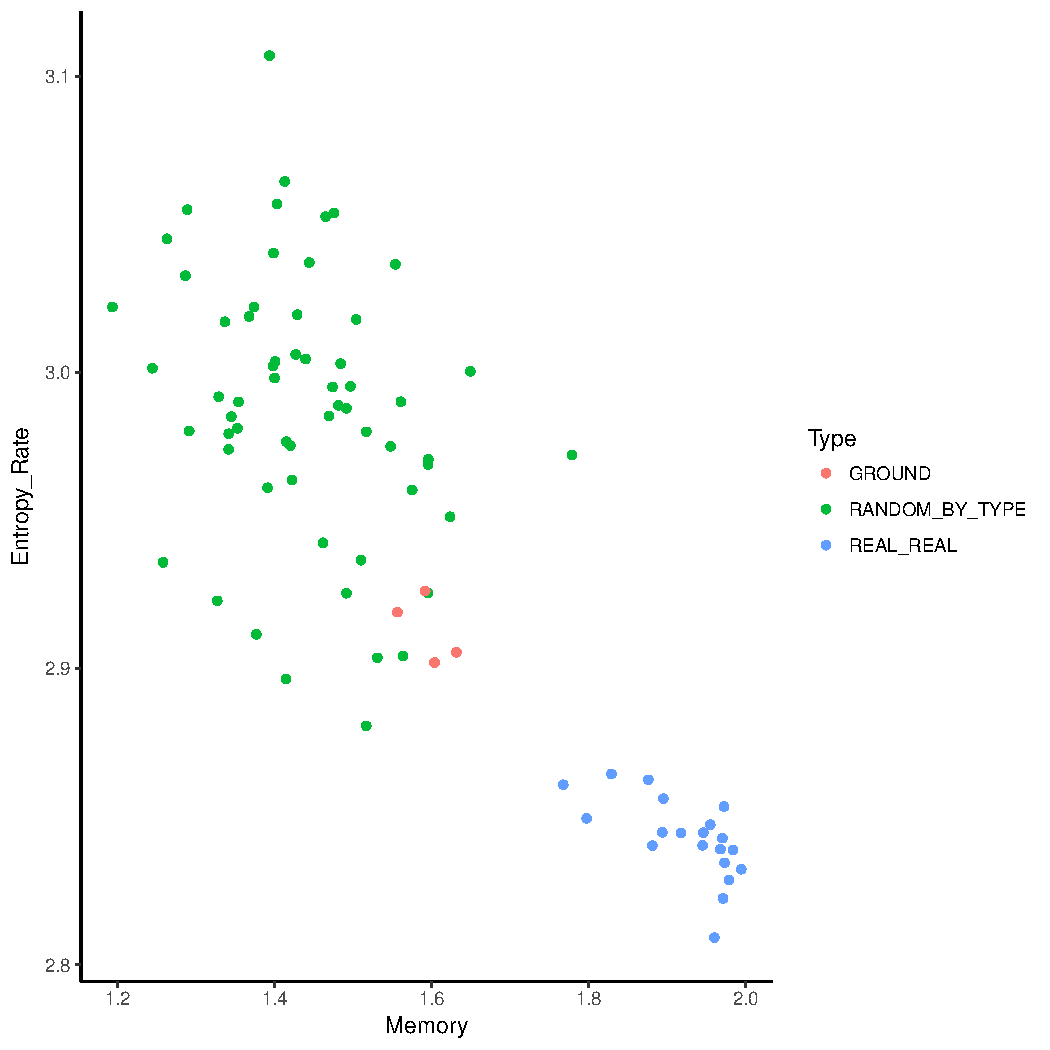
\includegraphics[width=0.25\textwidth]{figures/Afrikaans-entropy-memory.pdf}}  &  \multirow{4}{*}{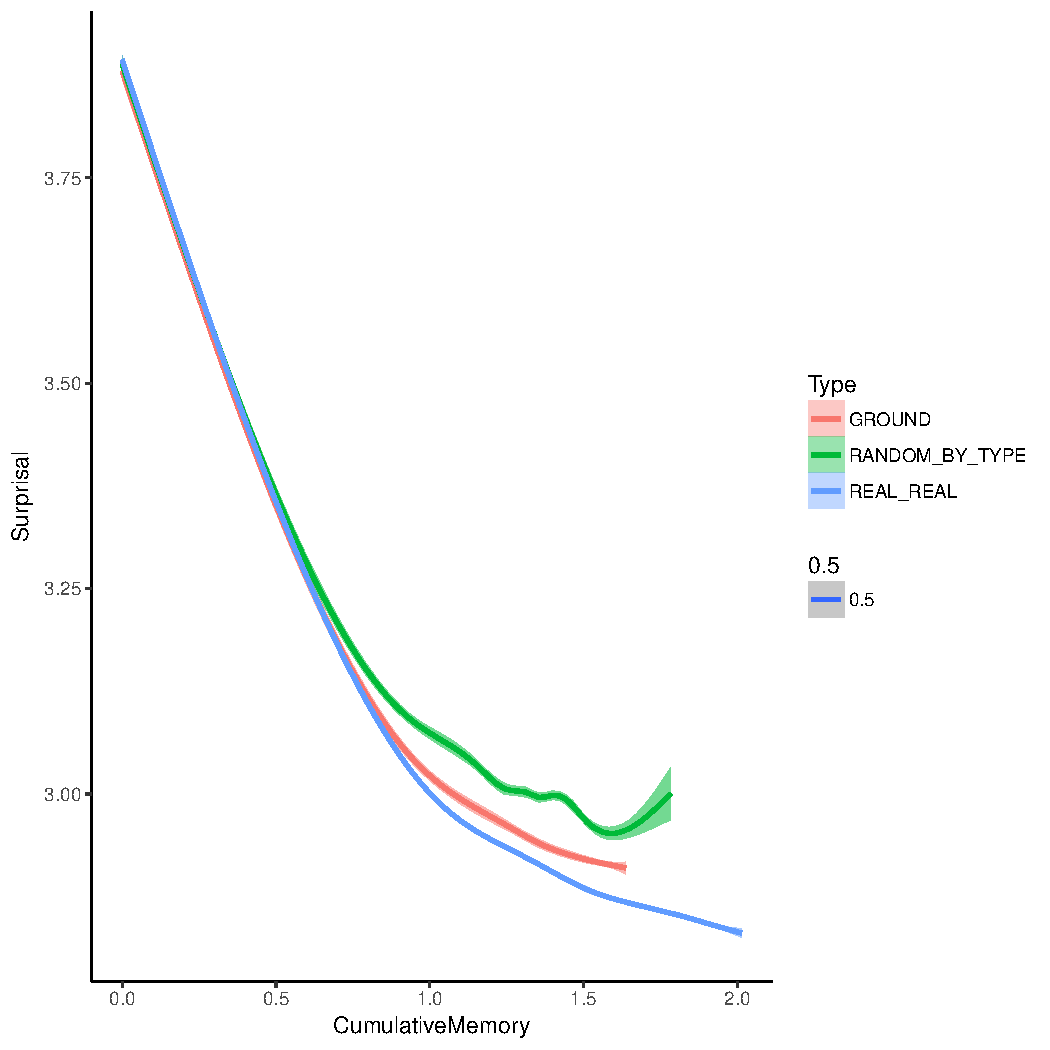
\includegraphics[width=0.25\textwidth]{figures/Afrikaans-listener-surprisal-memory.pdf}}  &  $D_x$  &  0.13  &  [0.05, 0.28]  \\ 
1315  &    &    &  $B_x-A_x$  &  0.0  &  [-0.0, 0.01]  \\ 
  &    &    &  $E_x$  &  0.42  &  [0.0, 1.0]  \\ 
  &    &    &  $W_x$  &  0.99  &  [0.96, 1.0]  \\ [10.25ex] \hline
Amharic-Adap  &  \multirow{4}{*}{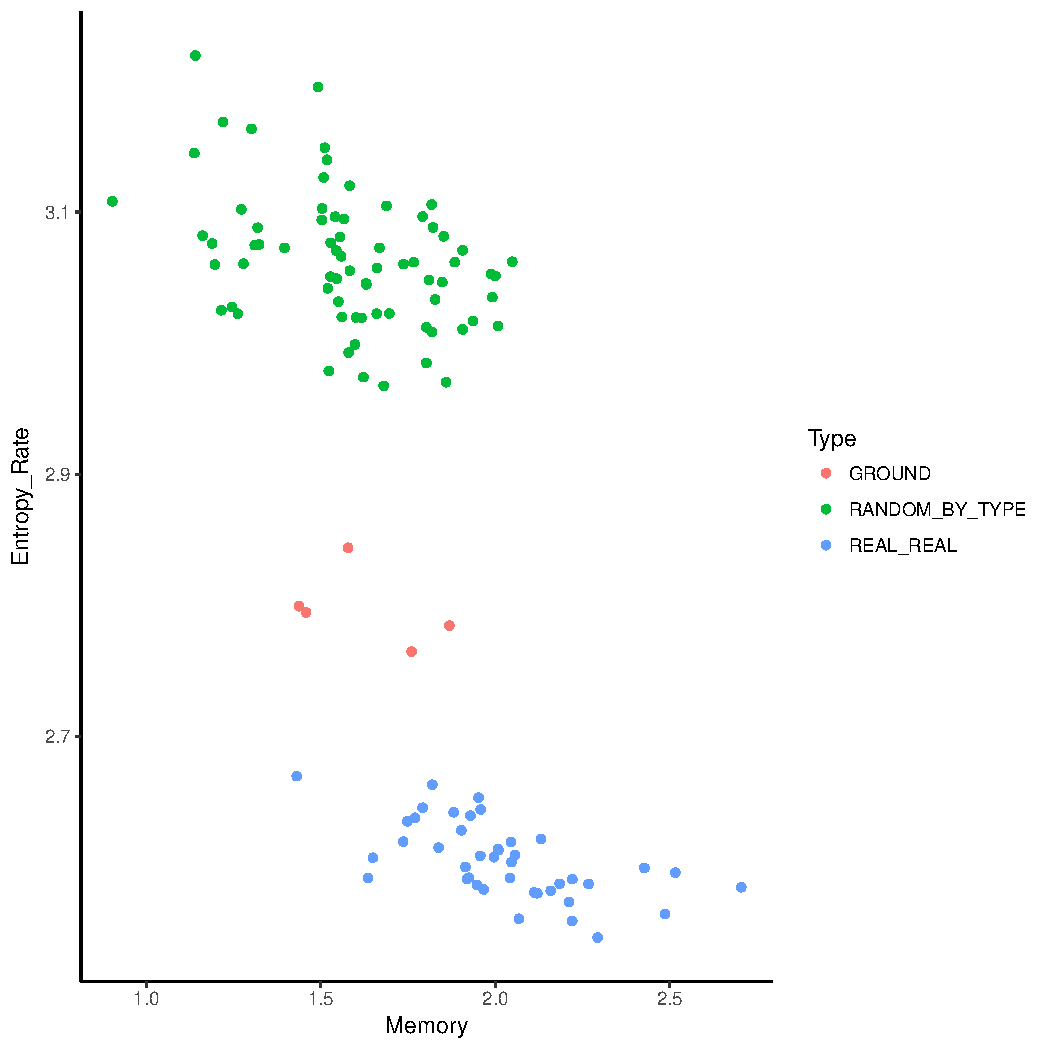
\includegraphics[width=0.25\textwidth]{figures/Amharic-Adap-entropy-memory.pdf}}  &  \multirow{4}{*}{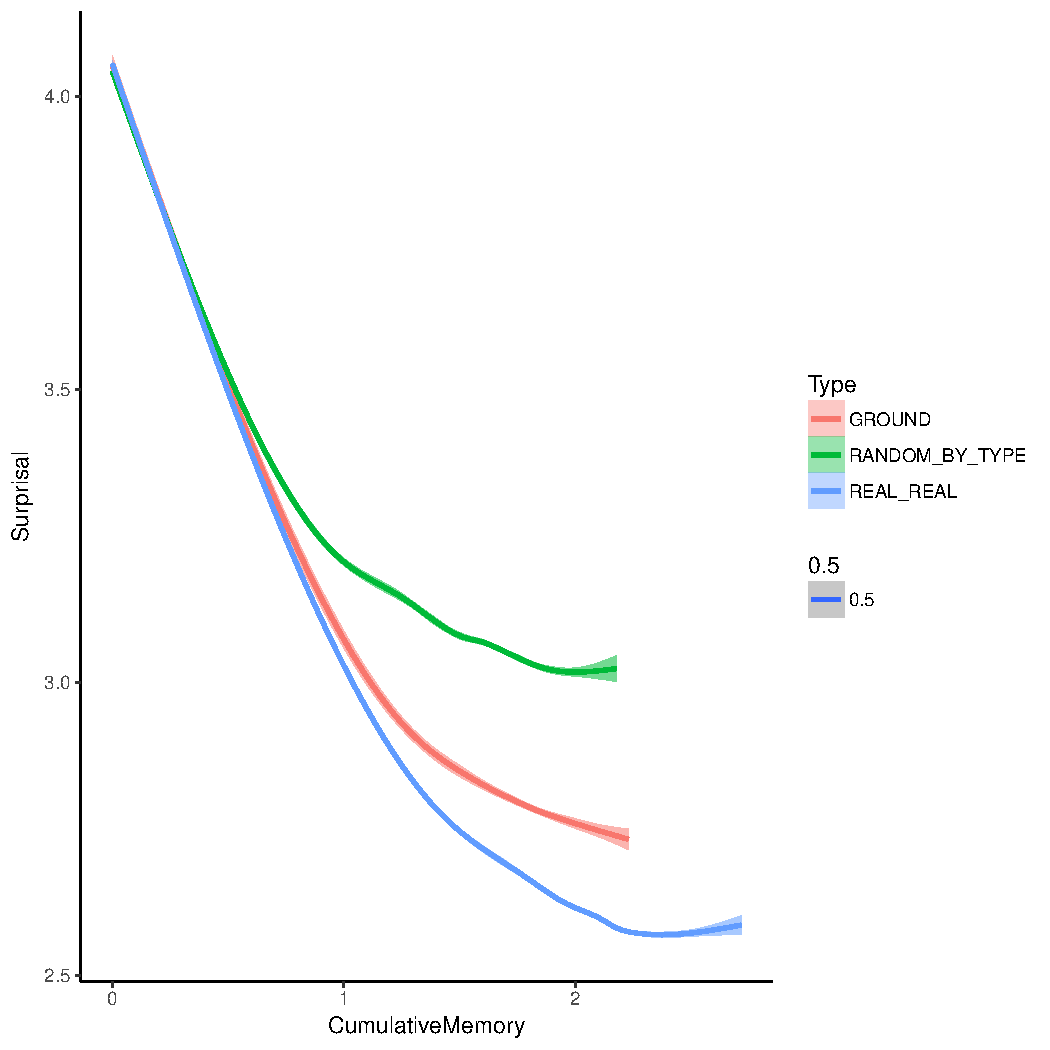
\includegraphics[width=0.25\textwidth]{figures/Amharic-Adap-listener-surprisal-memory.pdf}}  &  $D_x$  &  0.16  &  [0.06, 0.29]  \\ 
974  &    &    &  $B_x-A_x$  &  0.1  &  [0.04, 0.18]  \\ 
  &    &    &  $E_x$  &  1.0  &  [1.0, 1.0]  \\ 
  &    &    &  $W_x$  &  1.0  &  [1.0, 1.0]  \\ [10.25ex] \hline
Arabic*  &\\ [10.25ex] \hline
Armenian-Adap*  &\\ [10.25ex] \hline
Basque  &  \multirow{4}{*}{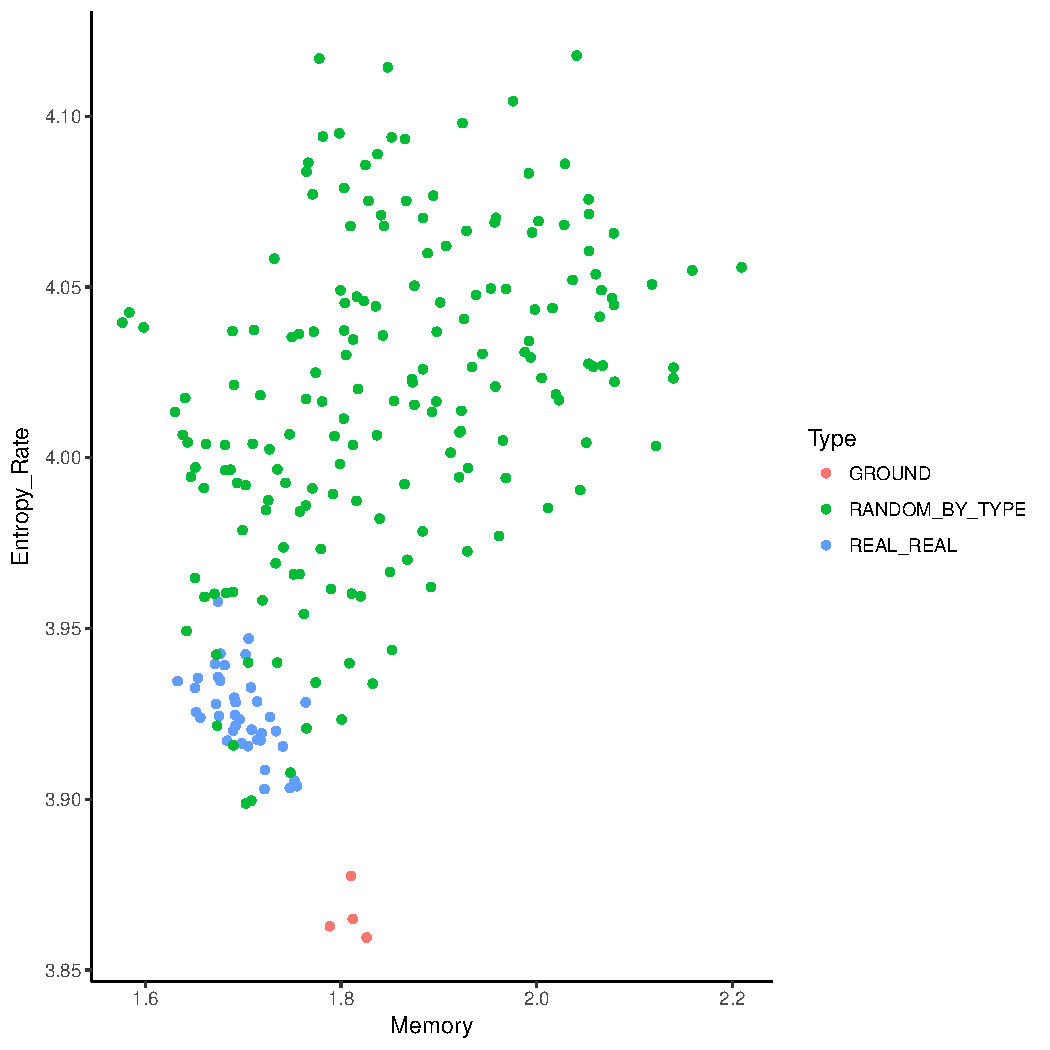
\includegraphics[width=0.25\textwidth]{figures/Basque-entropy-memory.pdf}}  &  \multirow{4}{*}{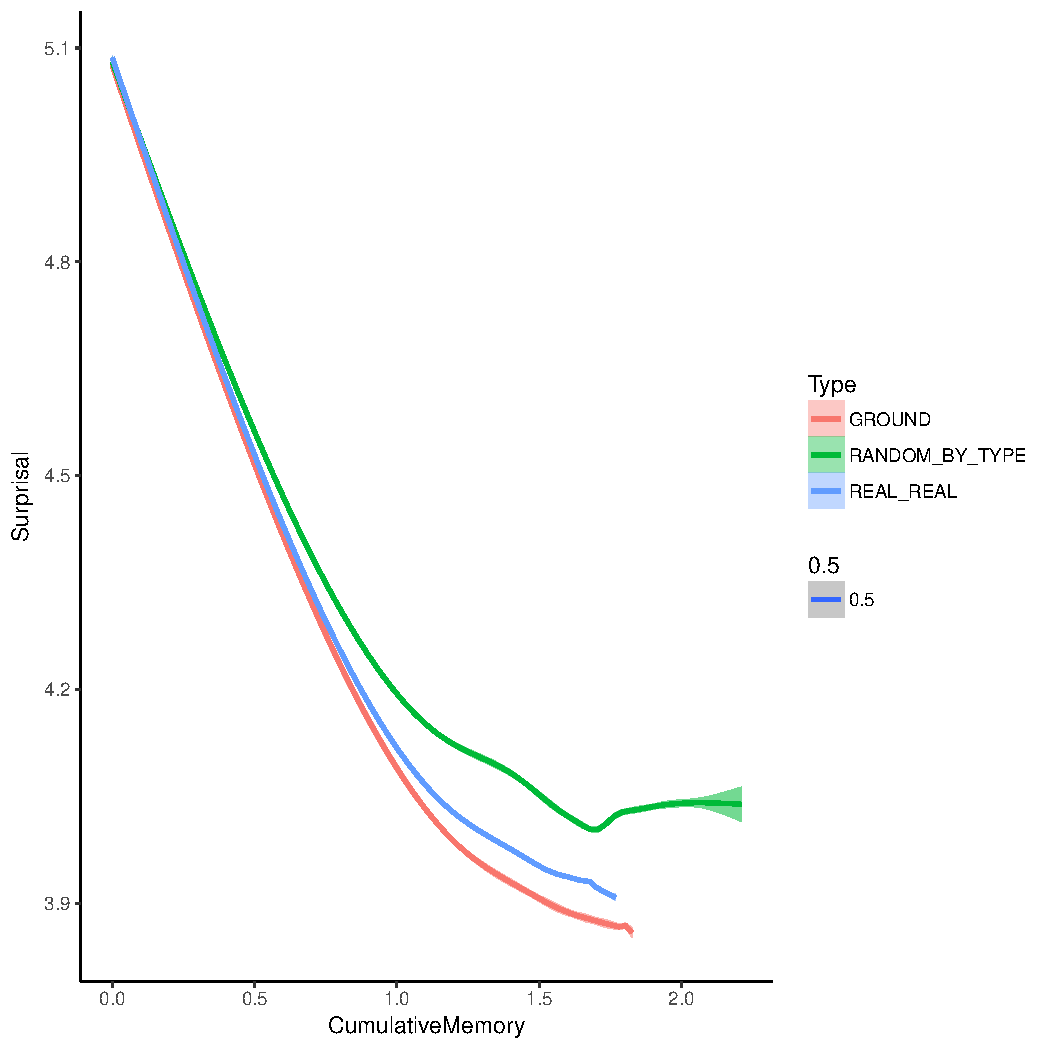
\includegraphics[width=0.25\textwidth]{figures/Basque-listener-surprisal-memory.pdf}}  &  $D_x$  &  0.09  &  [0.03, 0.15]  \\ 
5396  &    &    &  $B_x-A_x$  &  0.82  &  [0.76, 0.88]  \\ 
  &    &    &  $E_x$  &  0.99  &  [0.97, 1.0]  \\ 
  &    &    &  $W_x$  &  1.0  &  [1.0, 1.0]  \\ [10.25ex] \hline
Breton-Adap  &  \multirow{4}{*}{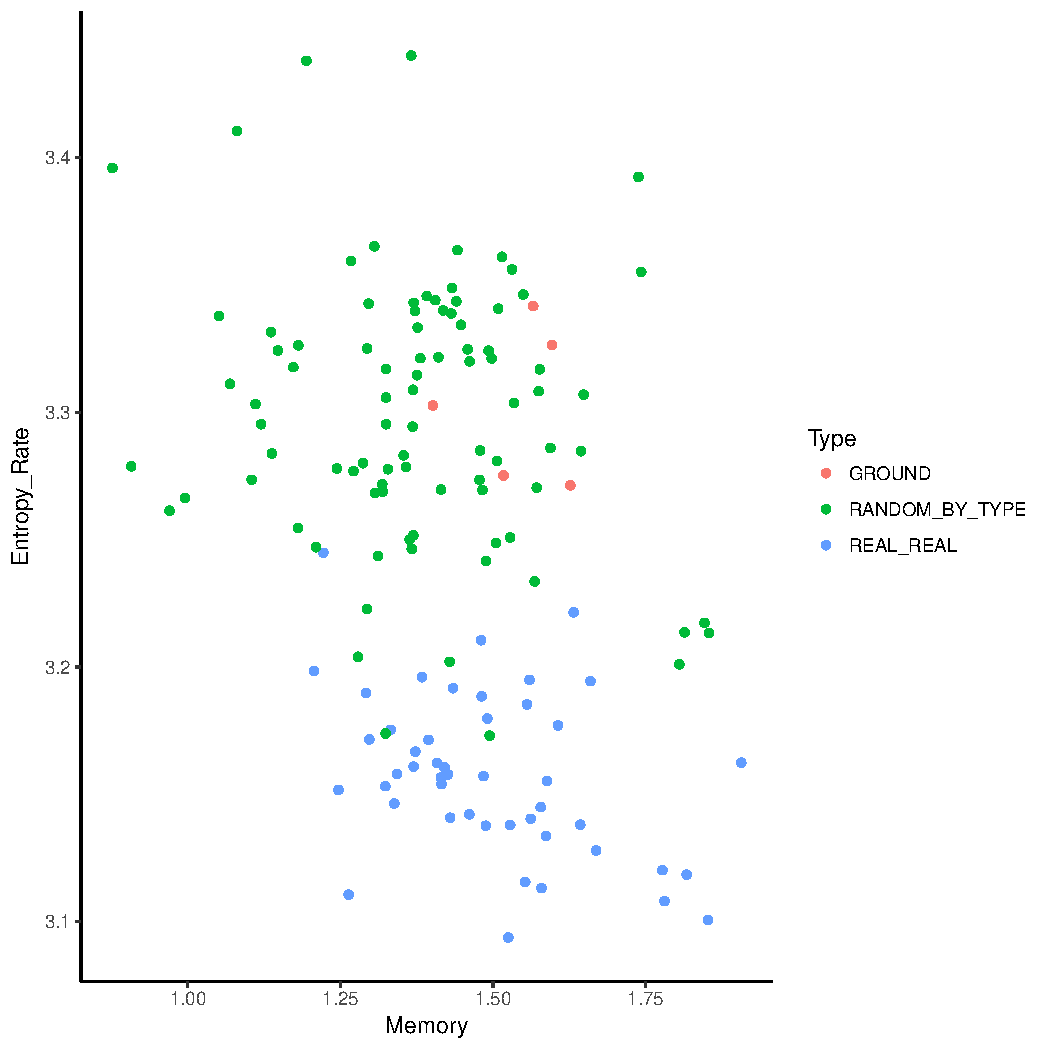
\includegraphics[width=0.25\textwidth]{figures/Breton-Adap-entropy-memory.pdf}}  &  \multirow{4}{*}{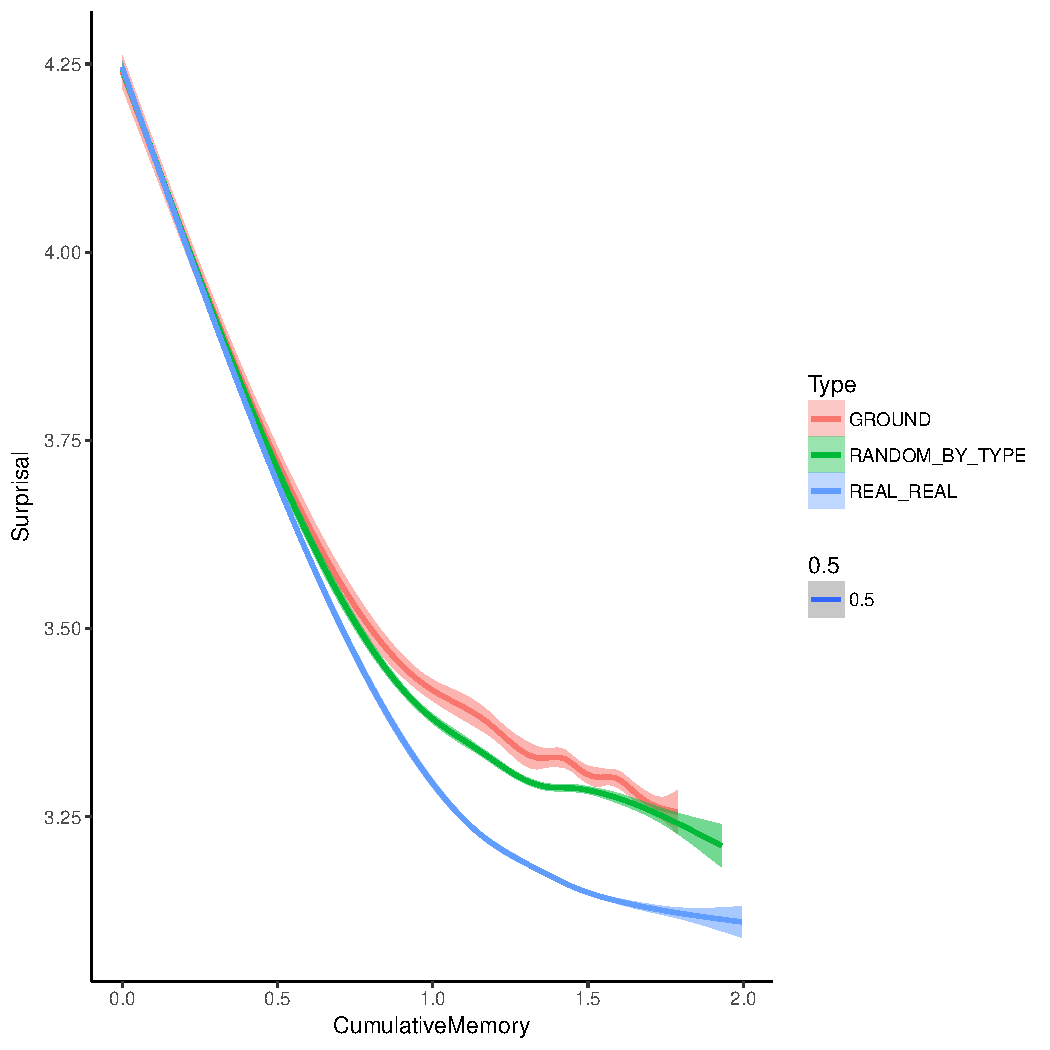
\includegraphics[width=0.25\textwidth]{figures/Breton-Adap-listener-surprisal-memory.pdf}}  &  $D_x$  &  0.11  &  [0.03, 0.22]  \\ 
788  &    &    &  $B_x-A_x$  &  0.32  &  [0.2, 0.42]  \\ 
  &    &    &  $E_x$  &  0.99  &  [0.95, 1.0]  \\ 
  &    &    &  $W_x$  &  1.0  &  [1.0, 1.0]  \\ [10.25ex] \hline
Bulgarian  &  \multirow{4}{*}{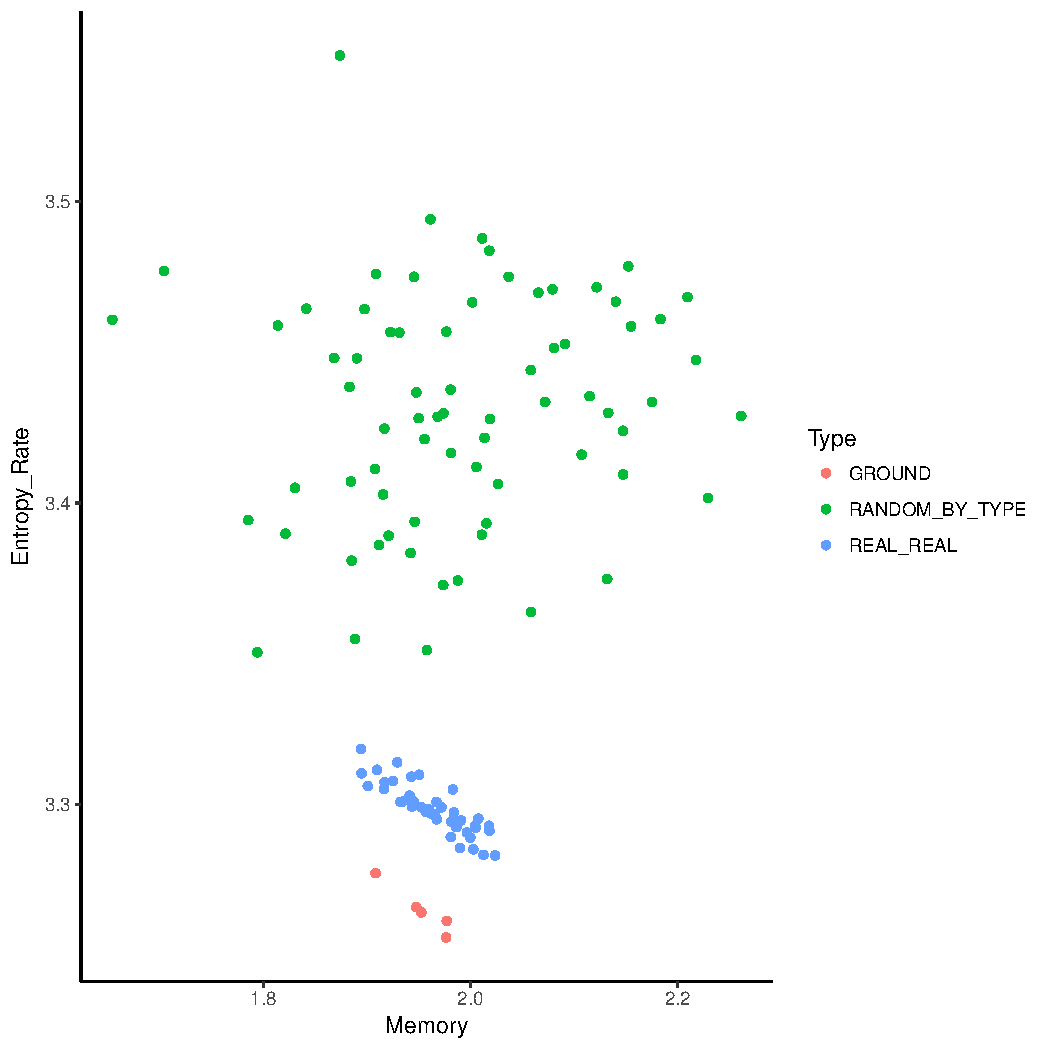
\includegraphics[width=0.25\textwidth]{figures/Bulgarian-entropy-memory.pdf}}  &  \multirow{4}{*}{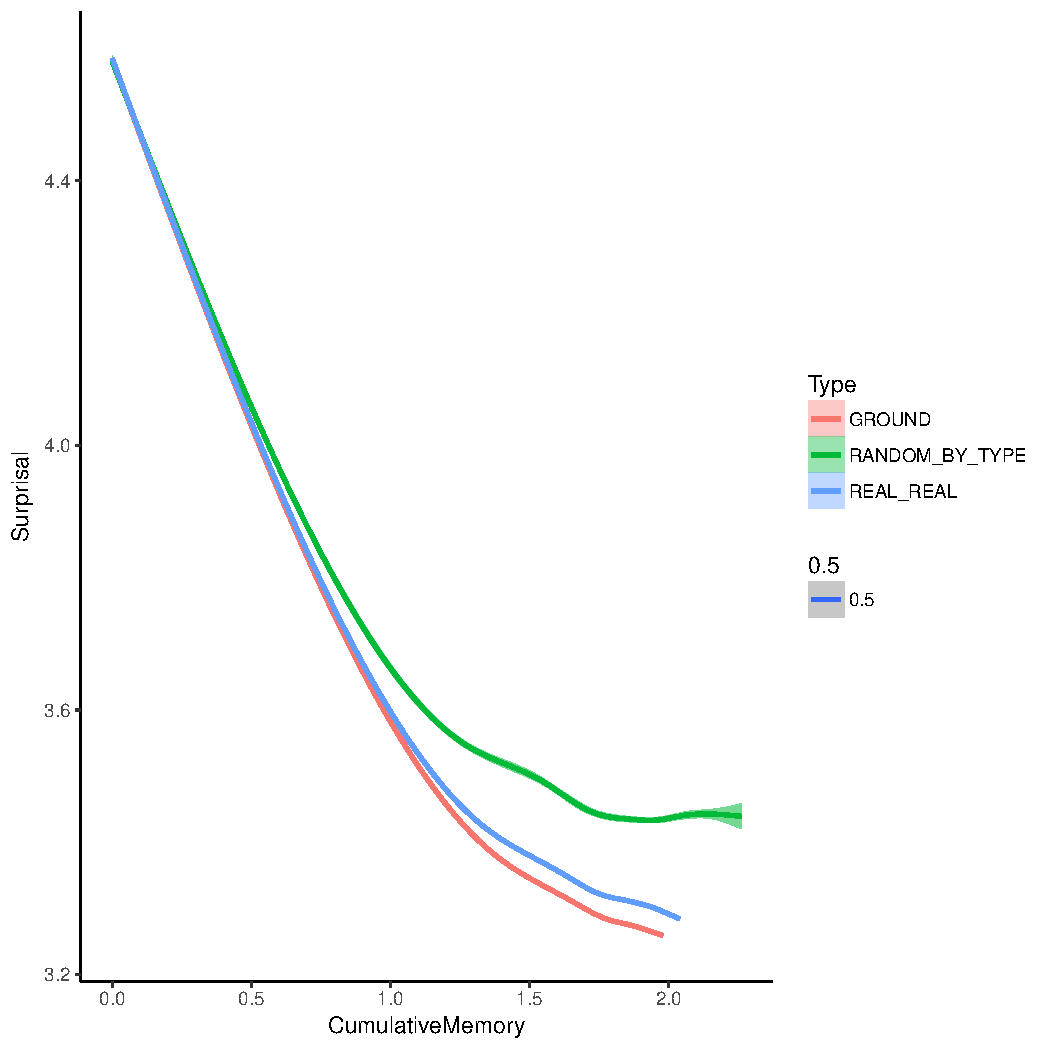
\includegraphics[width=0.25\textwidth]{figures/Bulgarian-listener-surprisal-memory.pdf}}  &  $D_x$  &  0.07  &  [0.0, 0.22]  \\ 
8907  &    &    &  $B_x-A_x$  &  0.56  &  [0.44, 0.7]  \\ 
  &    &    &  $E_x$  &  1.0  &  [1.0, 1.0]  \\ 
  &    &    &  $W_x$  &  1.0  &  [1.0, 1.0]  \\ [10.25ex] \hline
Buryat-Adap  &  \multirow{4}{*}{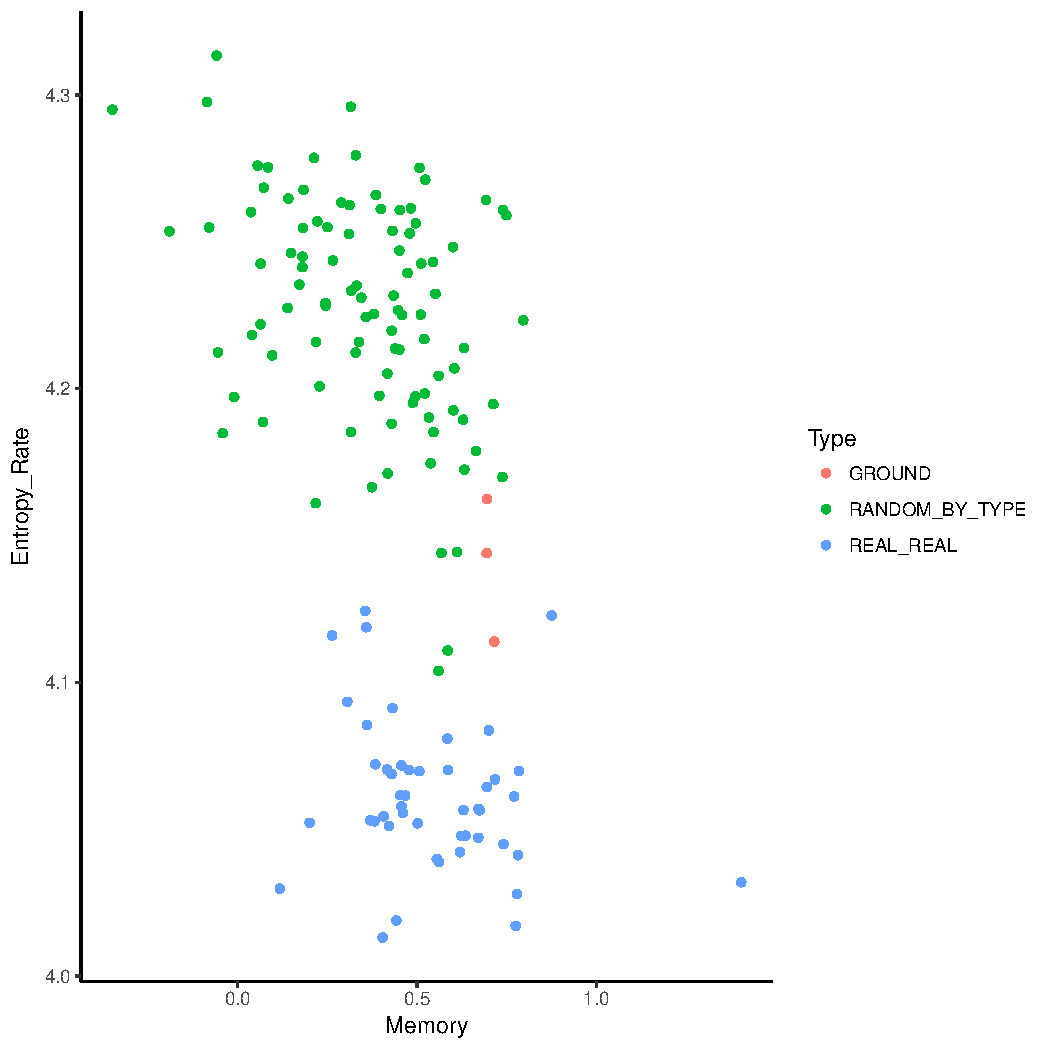
\includegraphics[width=0.25\textwidth]{figures/Buryat-Adap-entropy-memory.pdf}}  &  \multirow{4}{*}{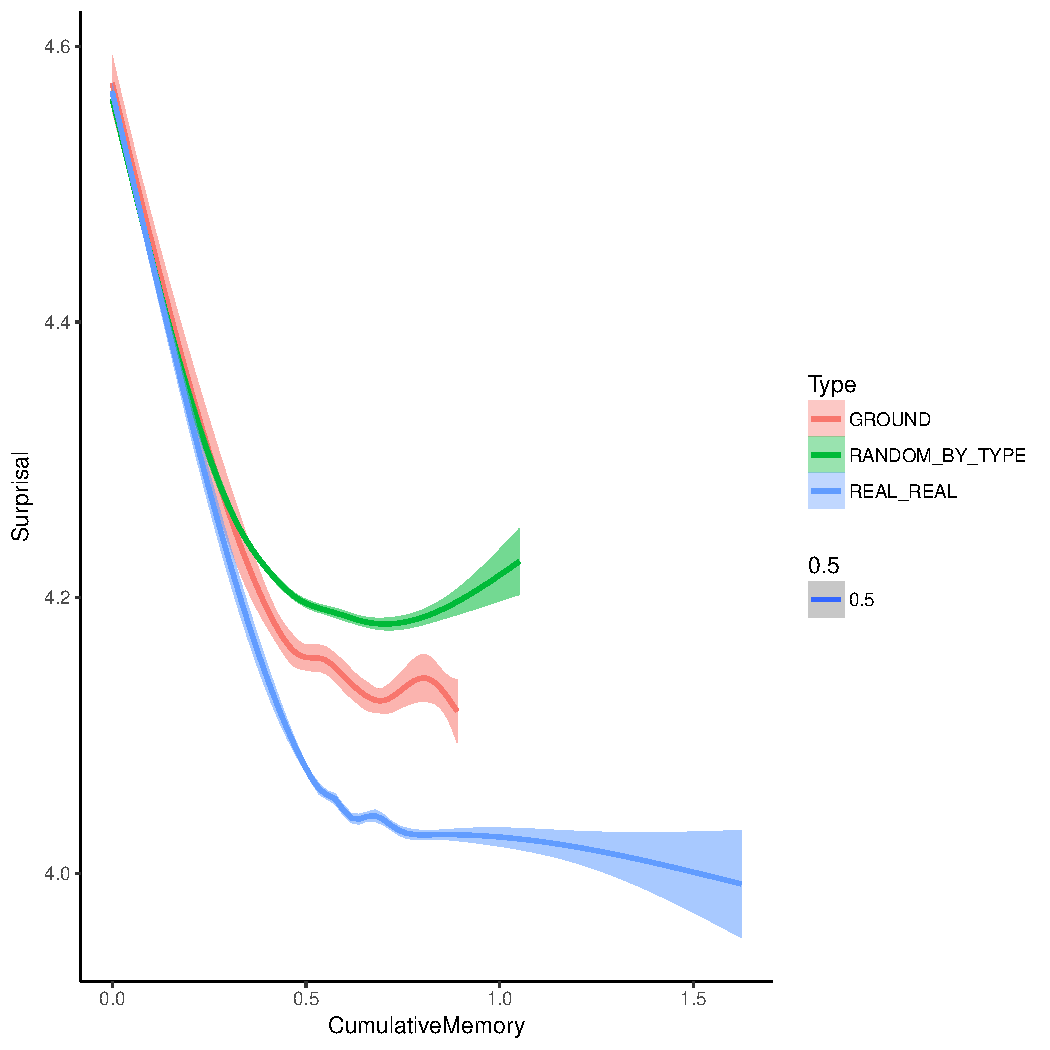
\includegraphics[width=0.25\textwidth]{figures/Buryat-Adap-listener-surprisal-memory.pdf}}  &  $D_x$  &  0.09  &  [0.02, 0.19]  \\ 
808  &    &    &  $B_x-A_x$  &  0.28  &  [0.19, 0.42]  \\ 
  &    &    &  $E_x$  &  1.0  &  [0.99, 1.0]  \\ 
  &    &    &  $W_x$  &  1.0  &  [1.0, 1.0]  \\ [10.25ex] \hline
Cantonese-Adap  &  \multirow{4}{*}{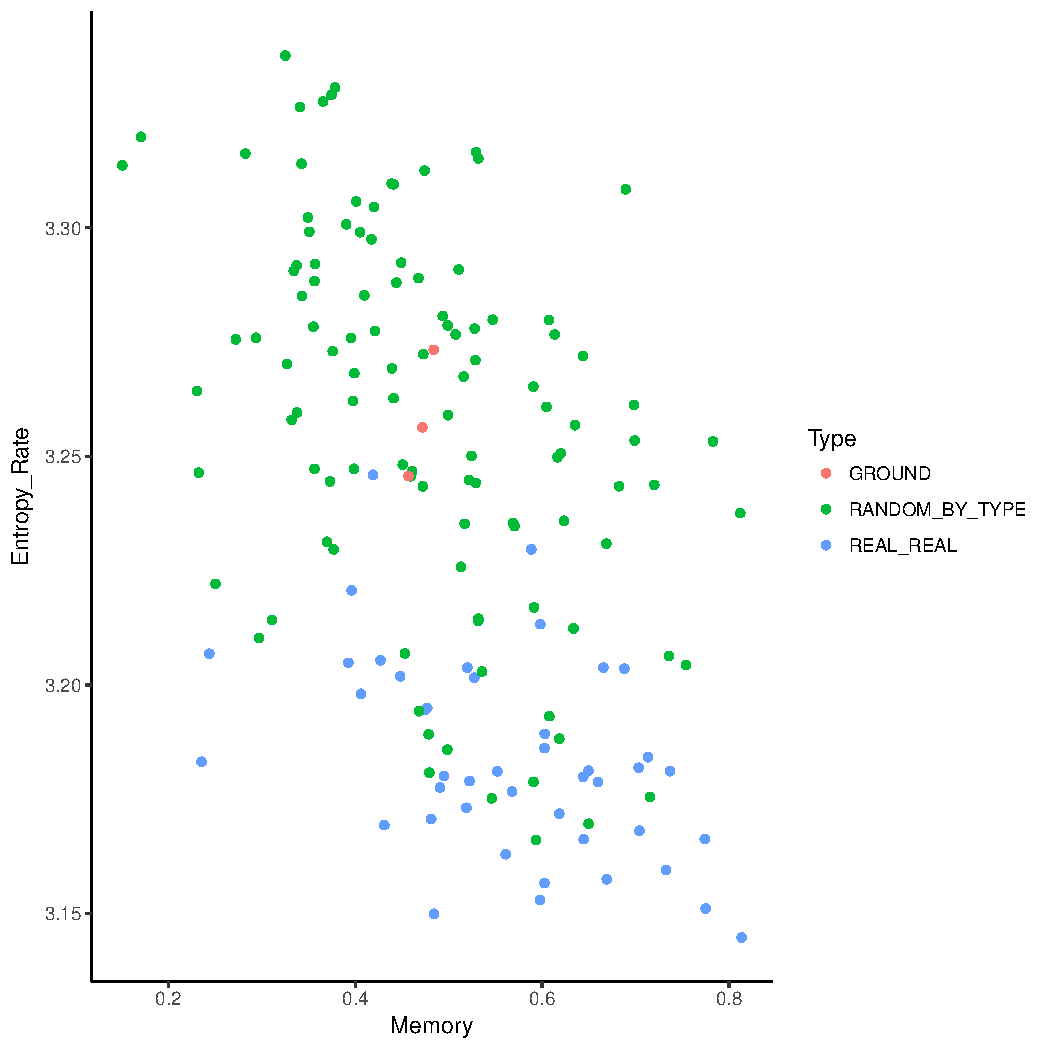
\includegraphics[width=0.25\textwidth]{figures/Cantonese-Adap-entropy-memory.pdf}}  &  \multirow{4}{*}{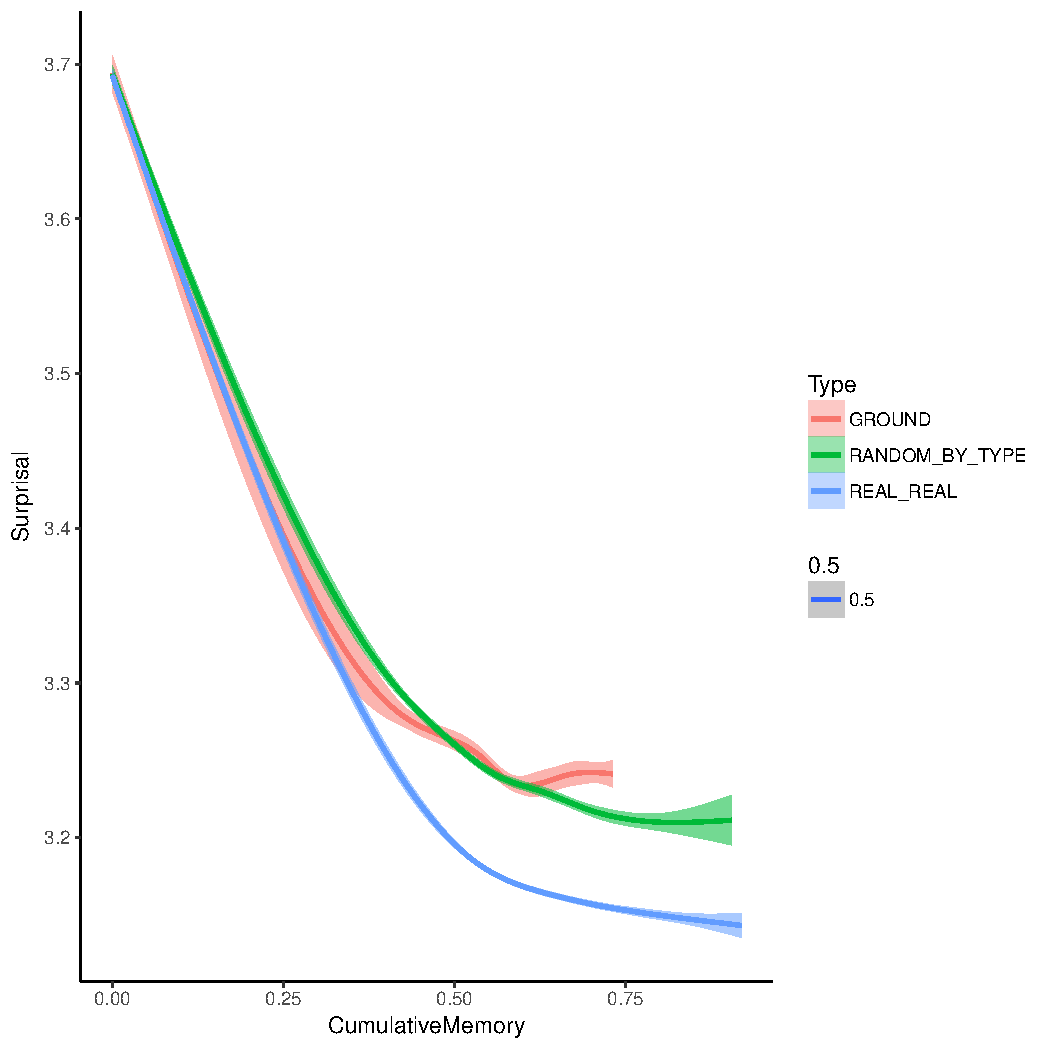
\includegraphics[width=0.25\textwidth]{figures/Cantonese-Adap-listener-surprisal-memory.pdf}}  &  $D_x$  &  0.17  &  [0.08, 0.31]  \\ 
550  &    &    &  $B_x-A_x$  &  0.25  &  [0.17, 0.36]  \\ 
  &    &    &  $E_x$  &  0.92  &  [0.85, 0.98]  \\ 
  &    &    &  $W_x$  &  0.94  &  [0.86, 1.0]  \\ [10.25ex] \hline
Catalan  &  \multirow{4}{*}{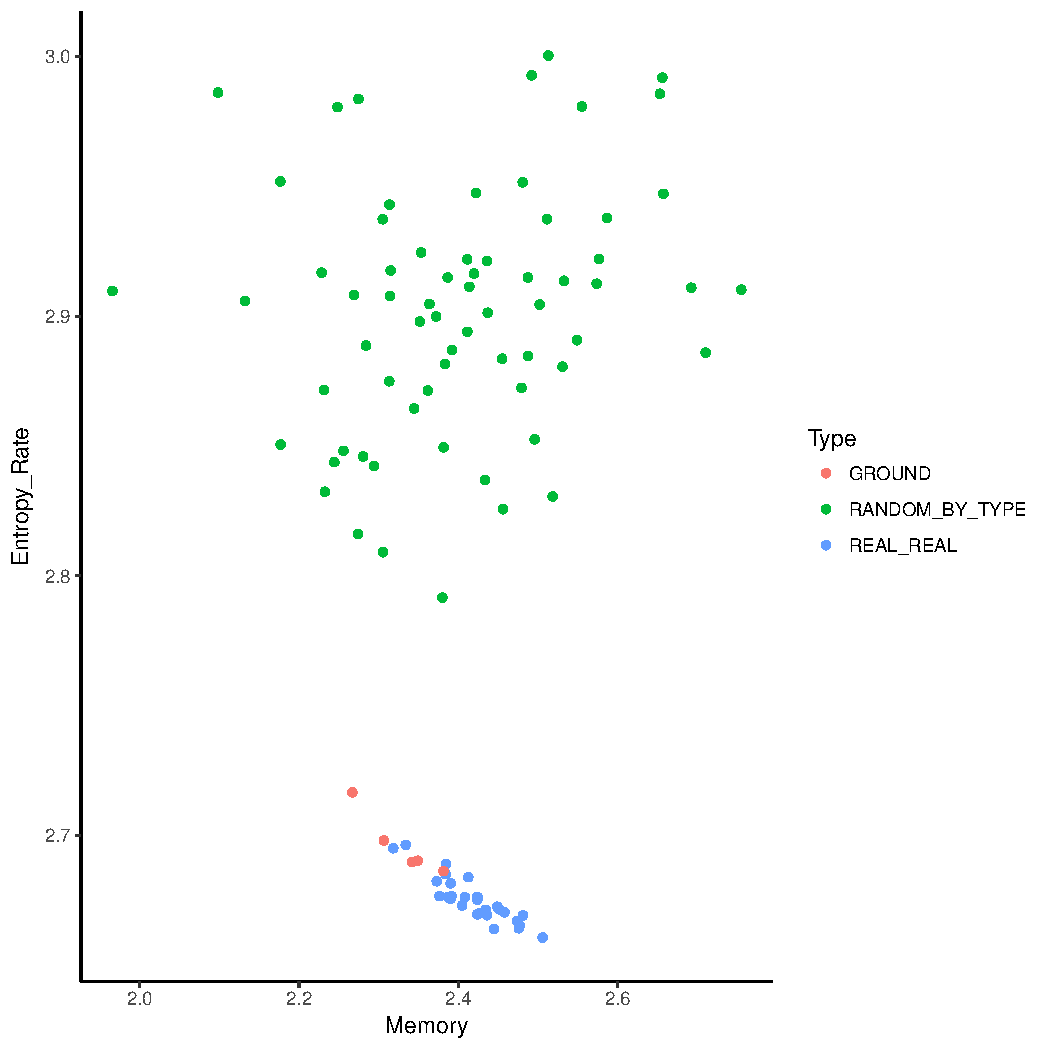
\includegraphics[width=0.25\textwidth]{figures/Catalan-entropy-memory.pdf}}  &  \multirow{4}{*}{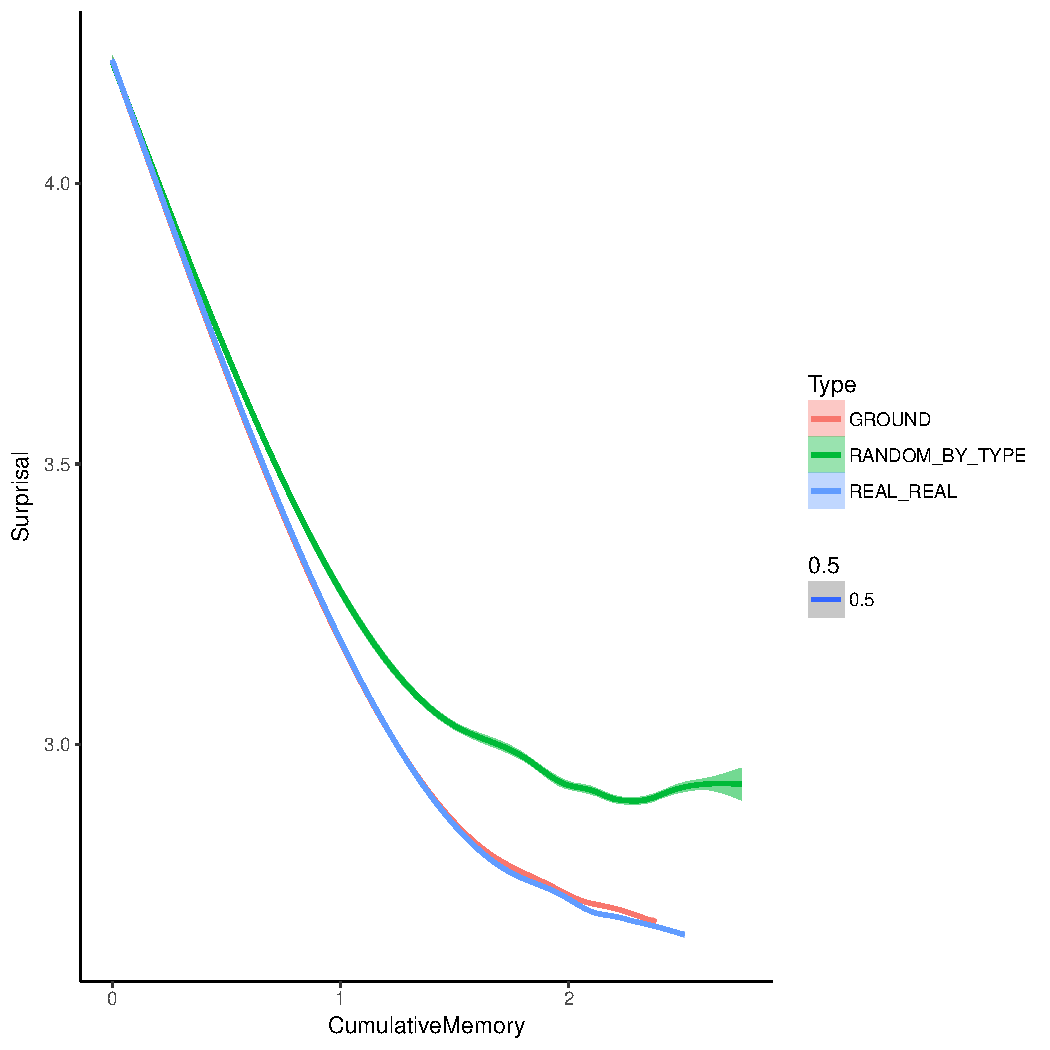
\includegraphics[width=0.25\textwidth]{figures/Catalan-listener-surprisal-memory.pdf}}  &  $D_x$  &  0.13  &  [0.03, 0.25]  \\ 
13123  &    &    &  $B_x-A_x$  &  0.44  &  [0.33, 0.57]  \\ 
  &    &    &  $E_x$  &  1.0  &  [1.0, 1.0]  \\ 
  &    &    &  $W_x$  &  1.0  &  [1.0, 1.0]  \\ [10.25ex] \hline
Chinese  &  \multirow{4}{*}{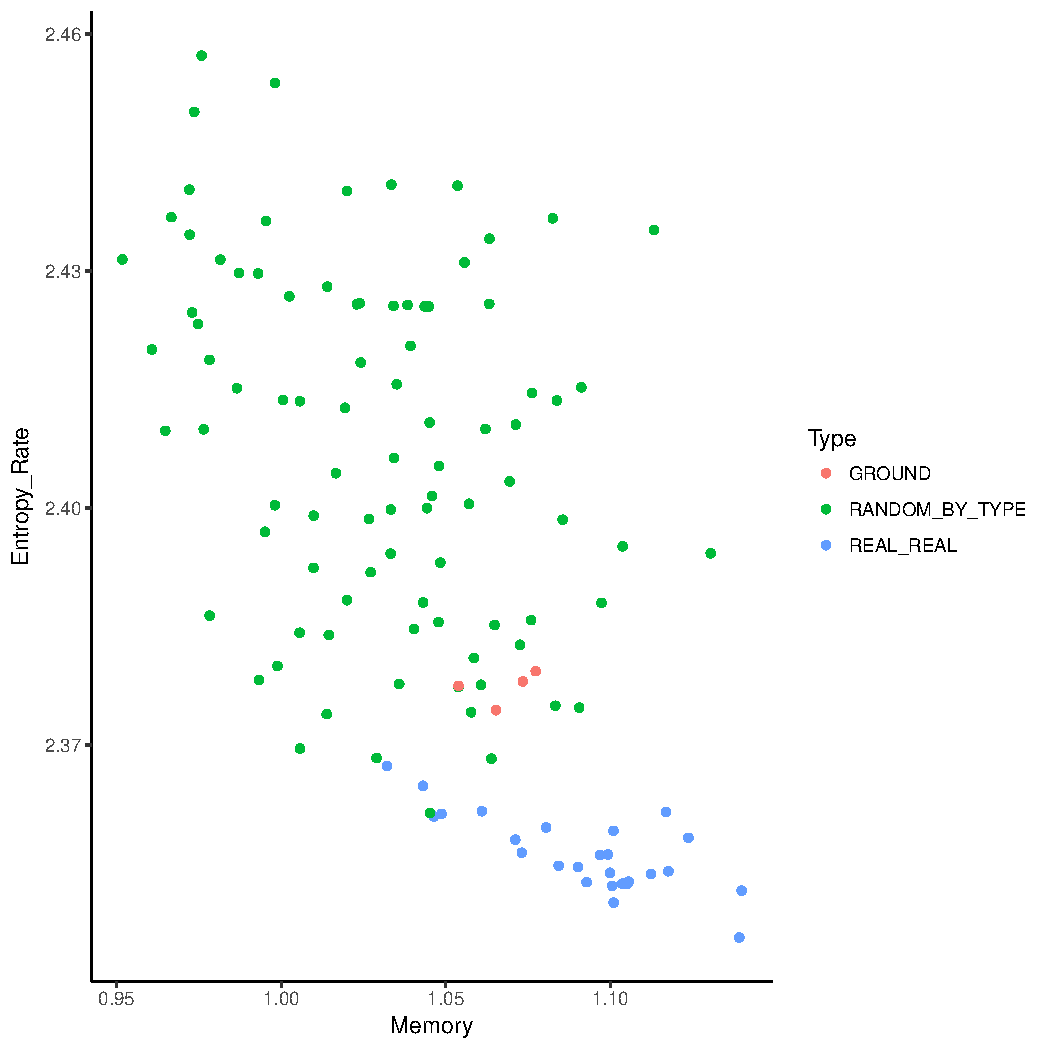
\includegraphics[width=0.25\textwidth]{figures/Chinese-entropy-memory.pdf}}  &  \multirow{4}{*}{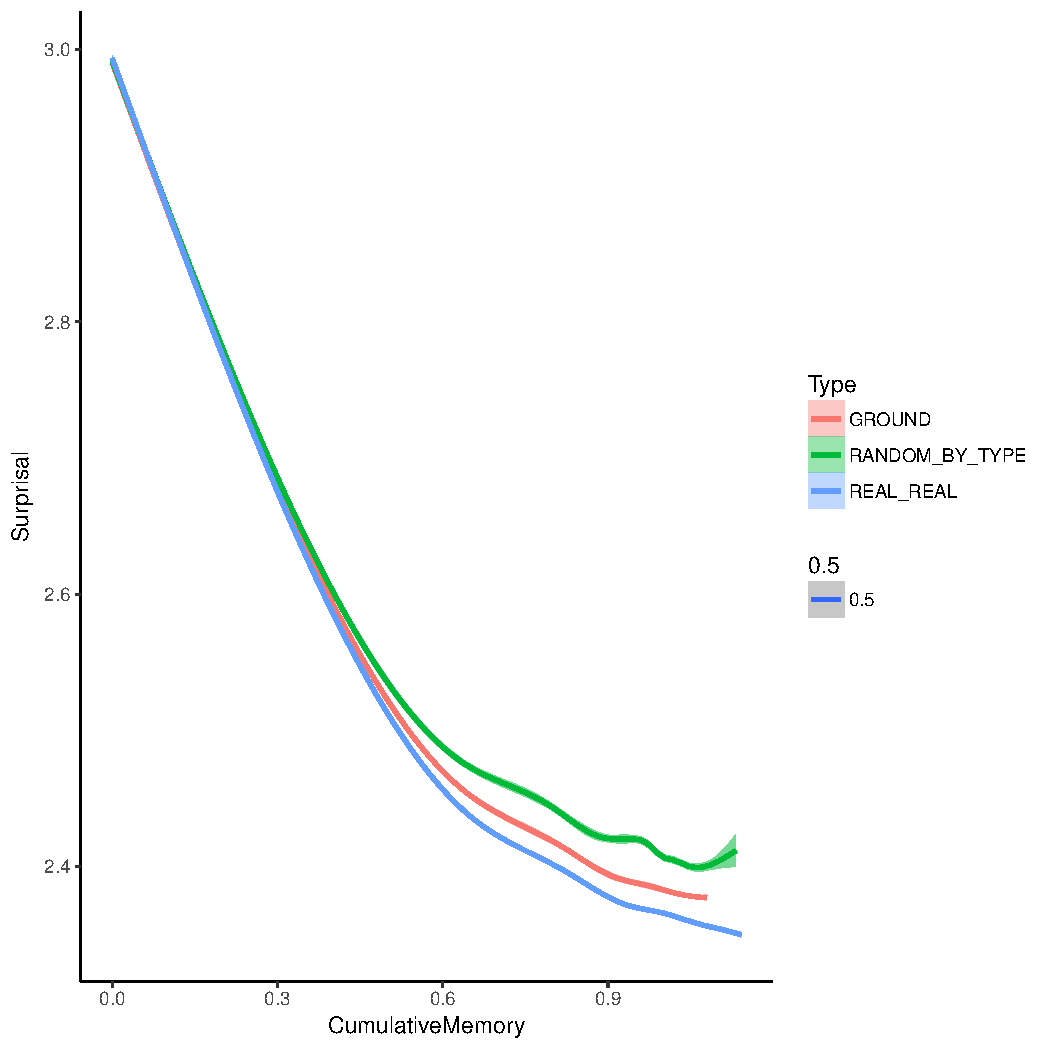
\includegraphics[width=0.25\textwidth]{figures/Chinese-listener-surprisal-memory.pdf}}  &  $D_x$  &  0.12  &  [0.04, 0.23]  \\ 
3997  &    &    &  $B_x-A_x$  &  0.1  &  [0.05, 0.19]  \\ 
  &    &    &  $E_x$  &  0.99  &  [0.95, 1.0]  \\ 
  &    &    &  $W_x$  &  1.0  &  [1.0, 1.0]  \\ [10.25ex] \hline
Croatian  &  \multirow{4}{*}{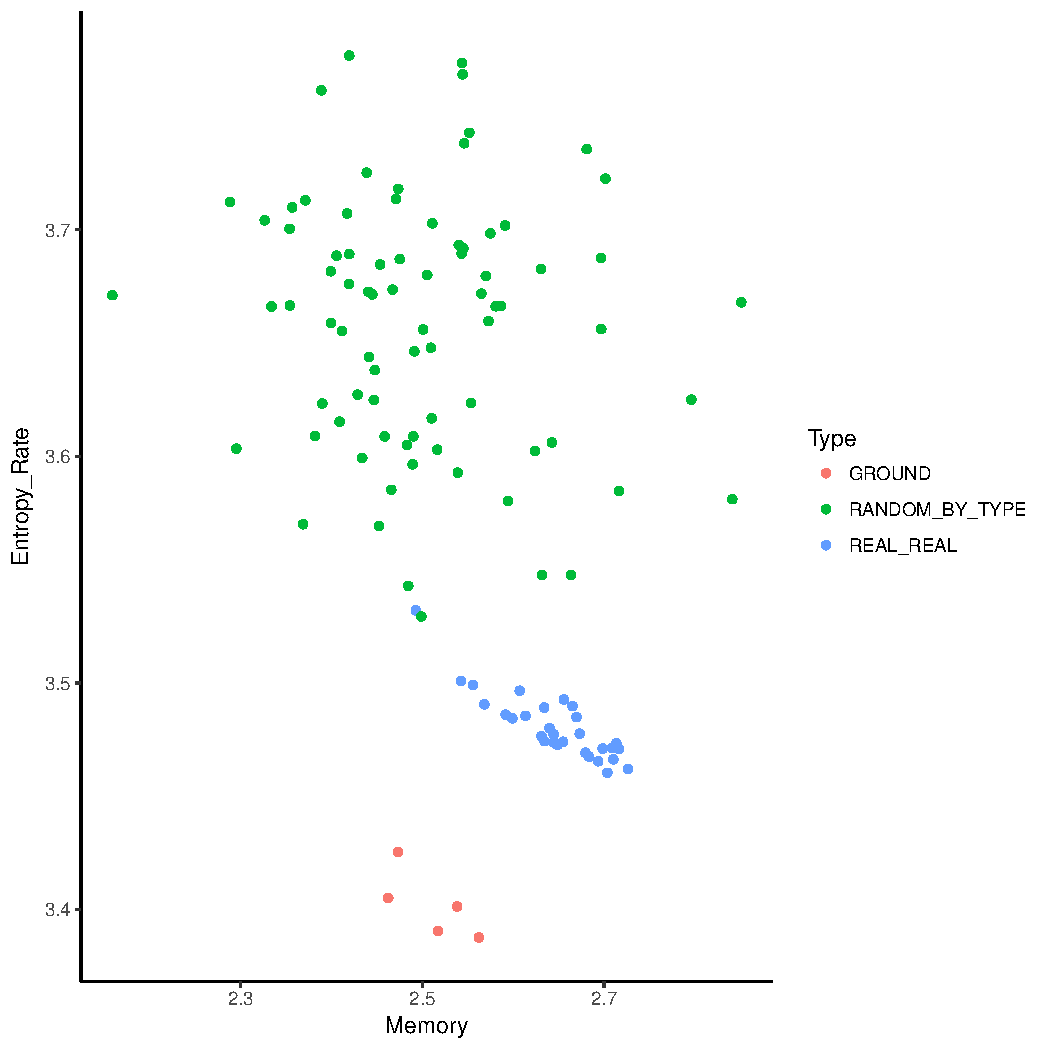
\includegraphics[width=0.25\textwidth]{figures/Croatian-entropy-memory.pdf}}  &  \multirow{4}{*}{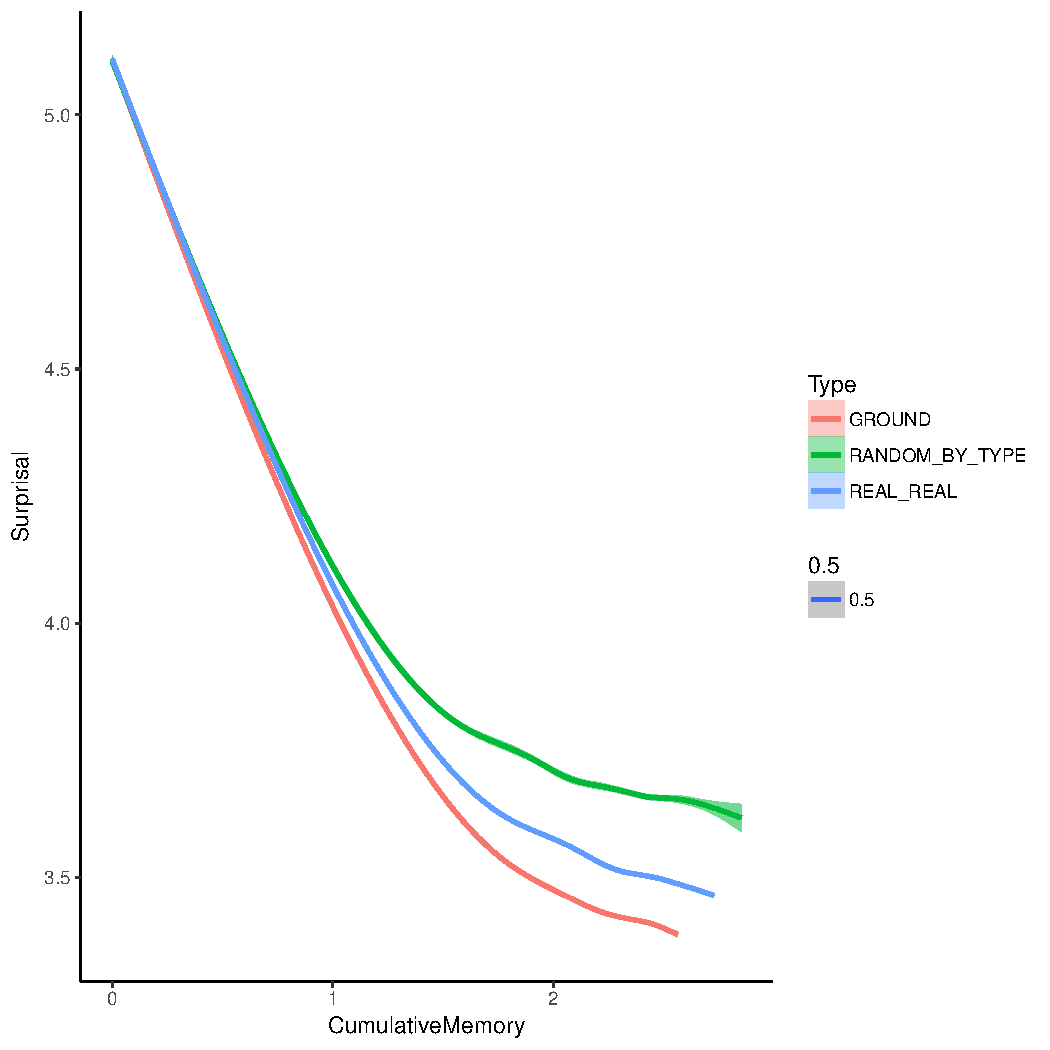
\includegraphics[width=0.25\textwidth]{figures/Croatian-listener-surprisal-memory.pdf}}  &  $D_x$  &  0.1  &  [0.03, 0.23]  \\ 
7689  &    &    &  $B_x-A_x$  &  0.13  &  [0.05, 0.23]  \\ 
  &    &    &  $E_x$  &  1.0  &  [1.0, 1.0]  \\ 
  &    &    &  $W_x$  &  1.0  &  [1.0, 1.0]  \\ [10.25ex] \hline
Czech  &  \multirow{4}{*}{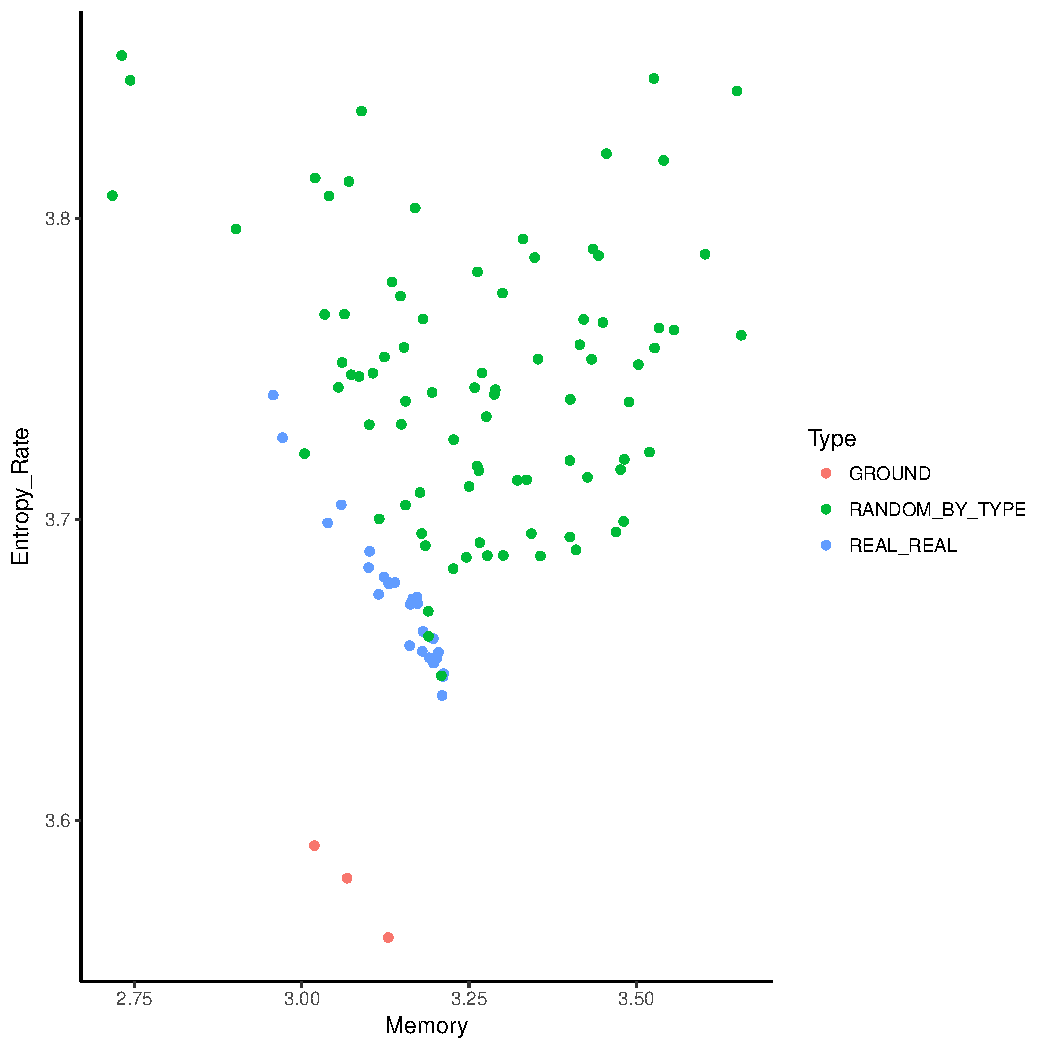
\includegraphics[width=0.25\textwidth]{figures/Czech-entropy-memory.pdf}}  &  \multirow{4}{*}{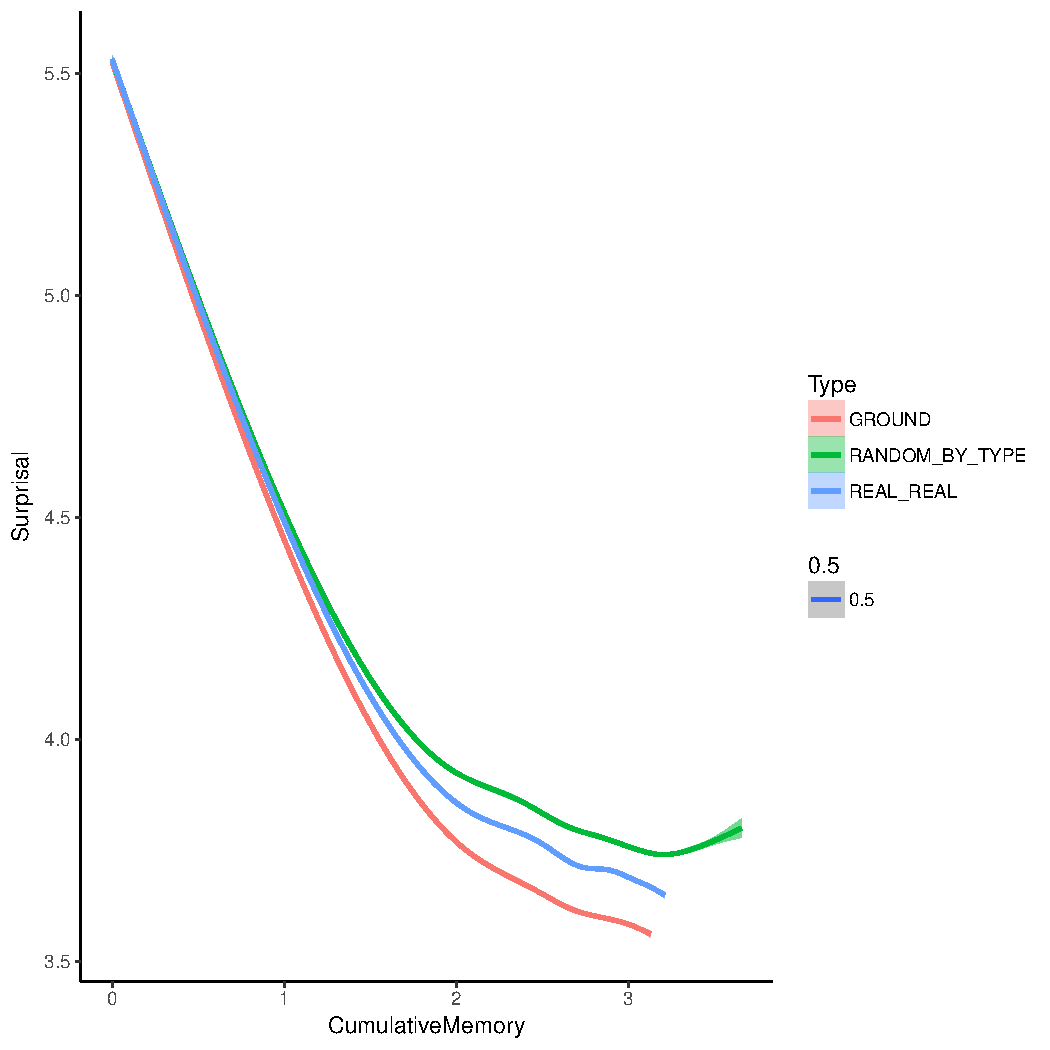
\includegraphics[width=0.25\textwidth]{figures/Czech-listener-surprisal-memory.pdf}}  &  $D_x$  &  0.14  &  [0.05, 0.27]  \\ 
102993  &    &    &  $B_x-A_x$  &  0.66  &  [0.56, 0.77]  \\ 
  &    &    &  $E_x$  &  1.0  &  [1.0, 1.0]  \\ 
  &    &    &  $W_x$  &  0.94  &  [0.86, 0.99]  \\ [10.25ex] \hline
Danish  &  \multirow{4}{*}{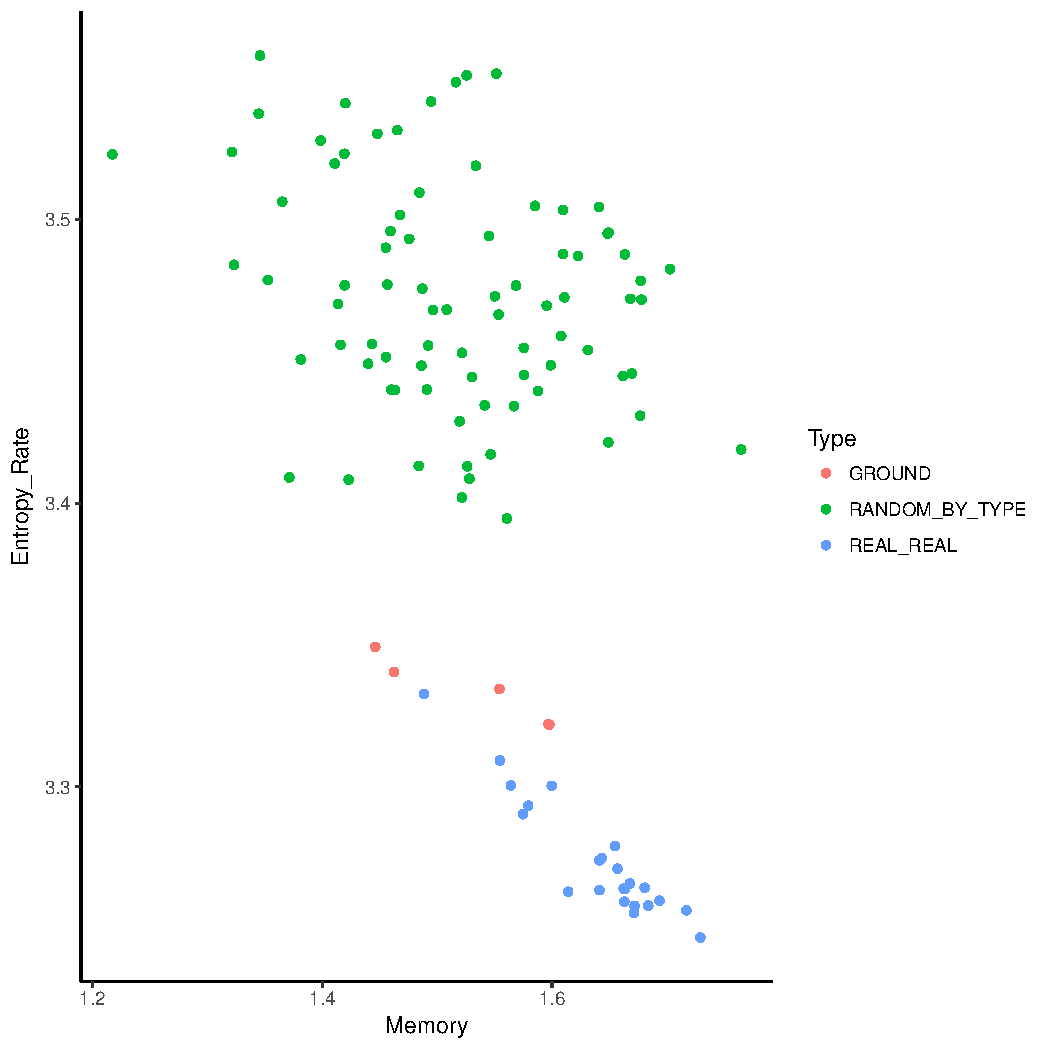
\includegraphics[width=0.25\textwidth]{figures/Danish-entropy-memory.pdf}}  &  \multirow{4}{*}{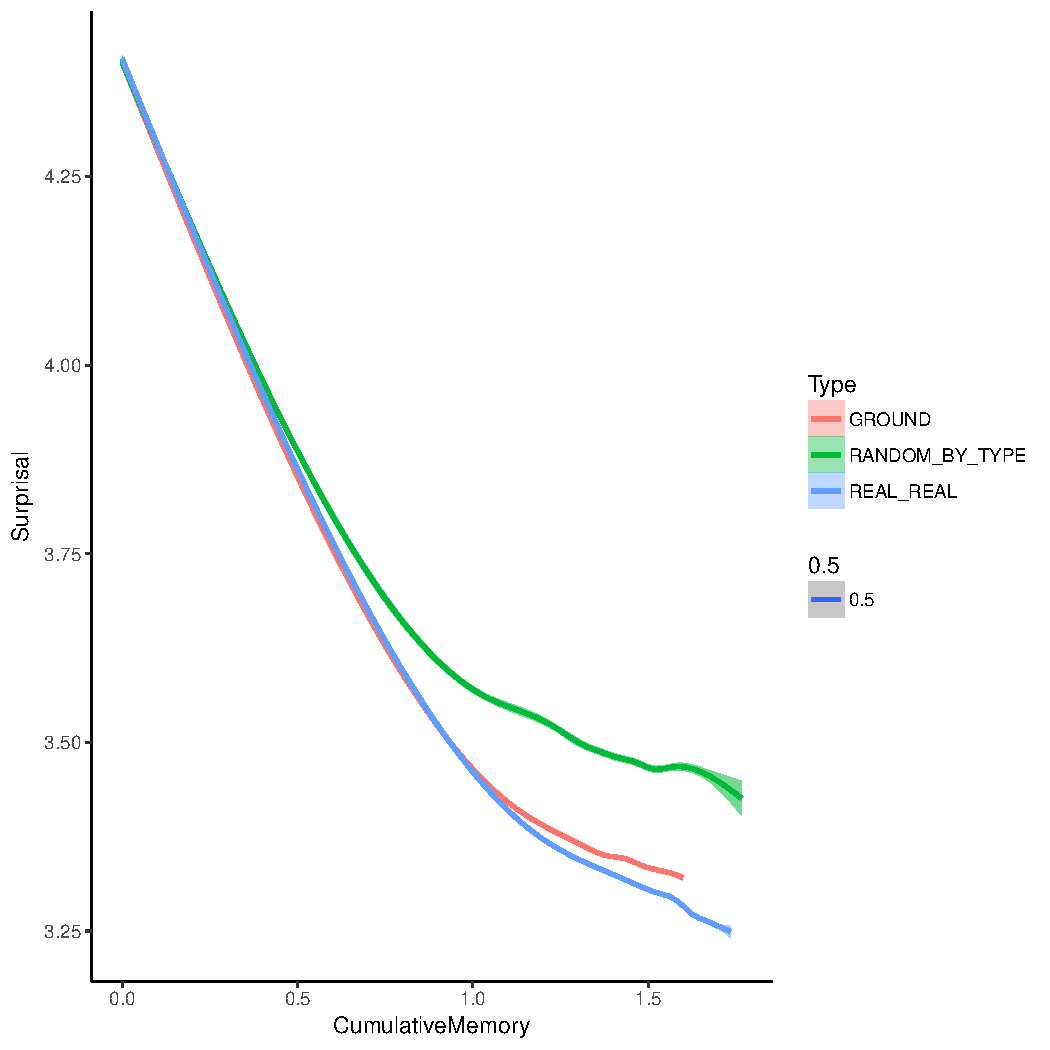
\includegraphics[width=0.25\textwidth]{figures/Danish-listener-surprisal-memory.pdf}}  &  $D_x$  &  0.11  &  [0.02, 0.26]  \\ 
4383  &    &    &  $B_x-A_x$  &  0.15  &  [0.06, 0.25]  \\ 
  &    &    &  $E_x$  &  1.0  &  [1.0, 1.0]  \\ 
  &    &    &  $W_x$  &  1.0  &  [1.0, 1.0]  \\ [10.25ex] \hline
Dutch  &  \multirow{4}{*}{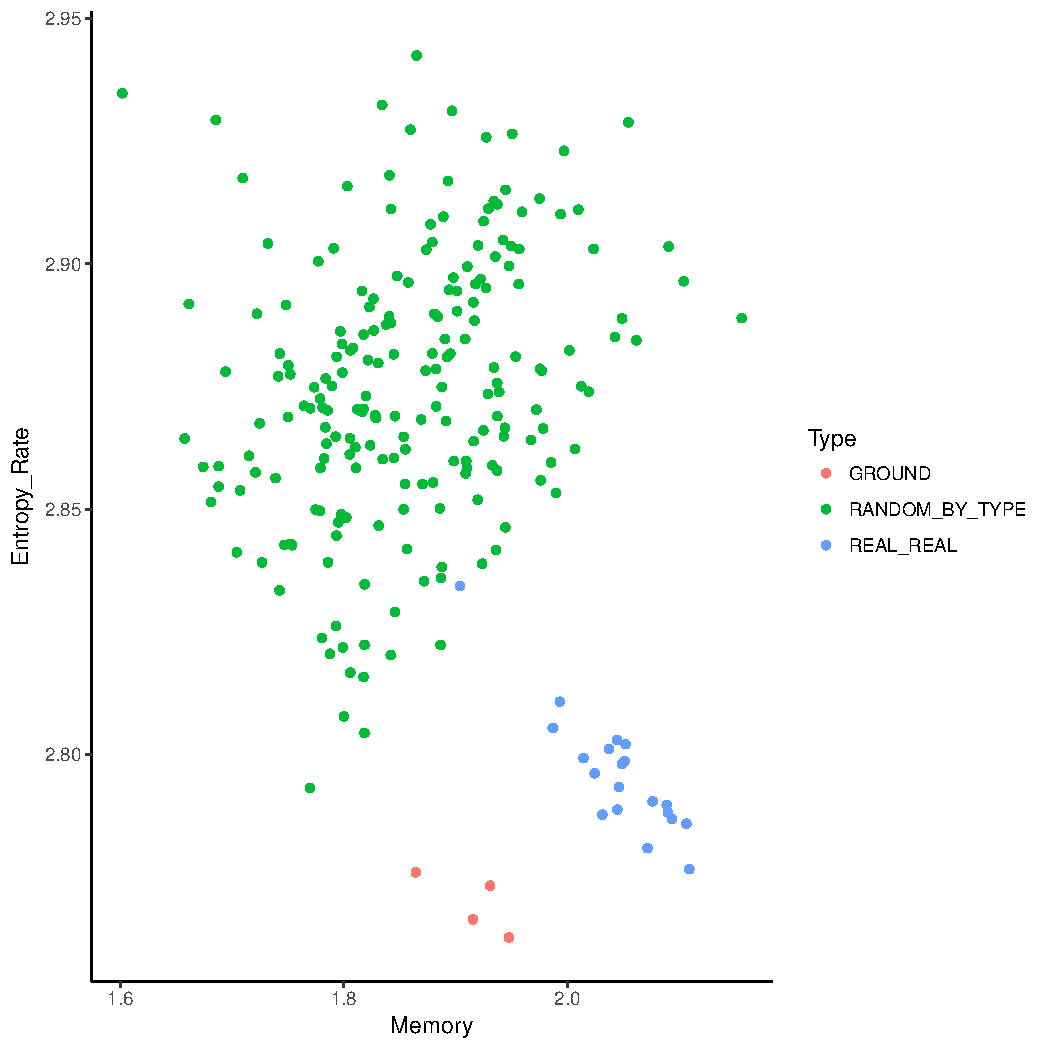
\includegraphics[width=0.25\textwidth]{figures/Dutch-entropy-memory.pdf}}  &  \multirow{4}{*}{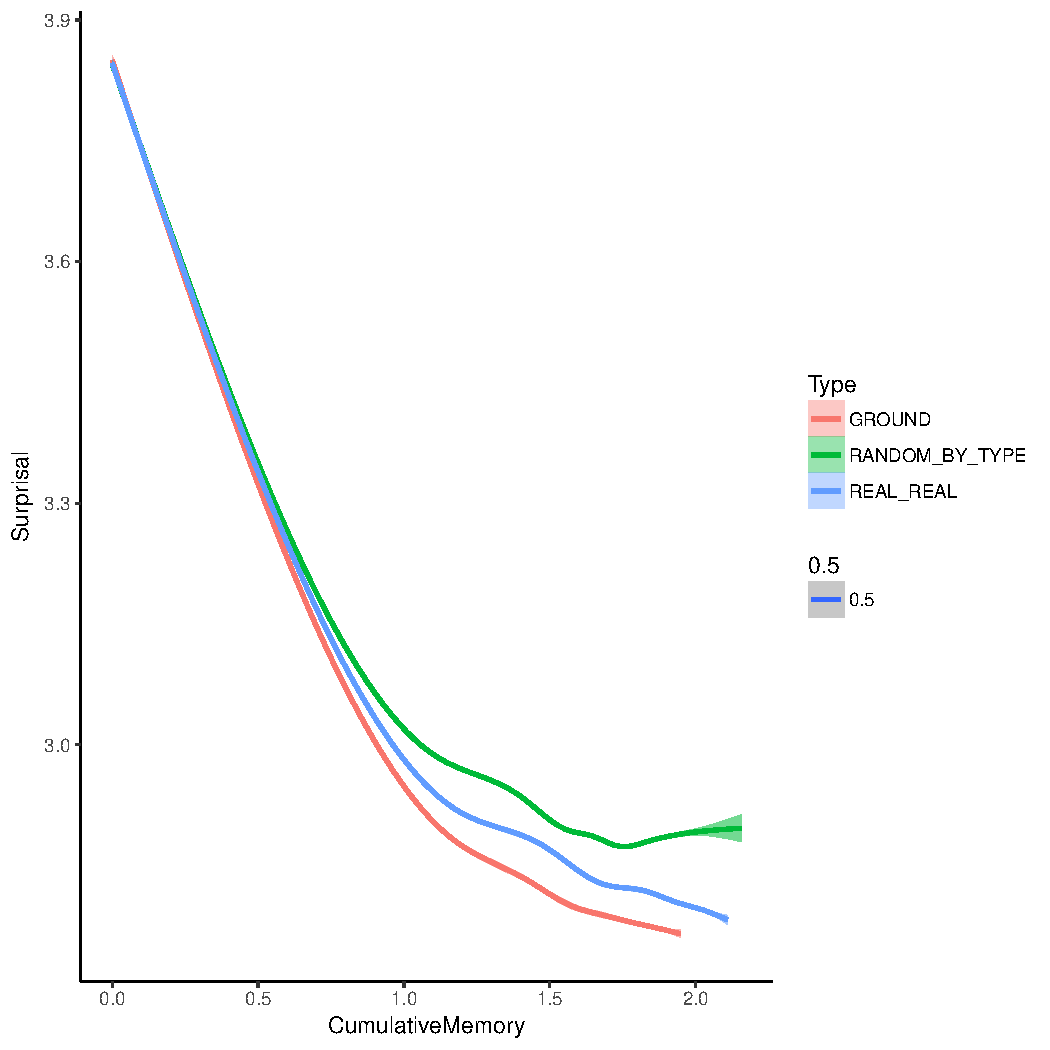
\includegraphics[width=0.25\textwidth]{figures/Dutch-listener-surprisal-memory.pdf}}  &  $D_x$  &  0.07  &  [0.01, 0.15]  \\ 
18310  &    &    &  $B_x-A_x$  &  0.04  &  [0.01, 0.08]  \\ 
  &    &    &  $E_x$  &  0.88  &  [0.73, 1.0]  \\ 
  &    &    &  $W_x$  &  0.98  &  [0.96, 1.0]  \\ [10.25ex] \hline
Estonian  &  \multirow{4}{*}{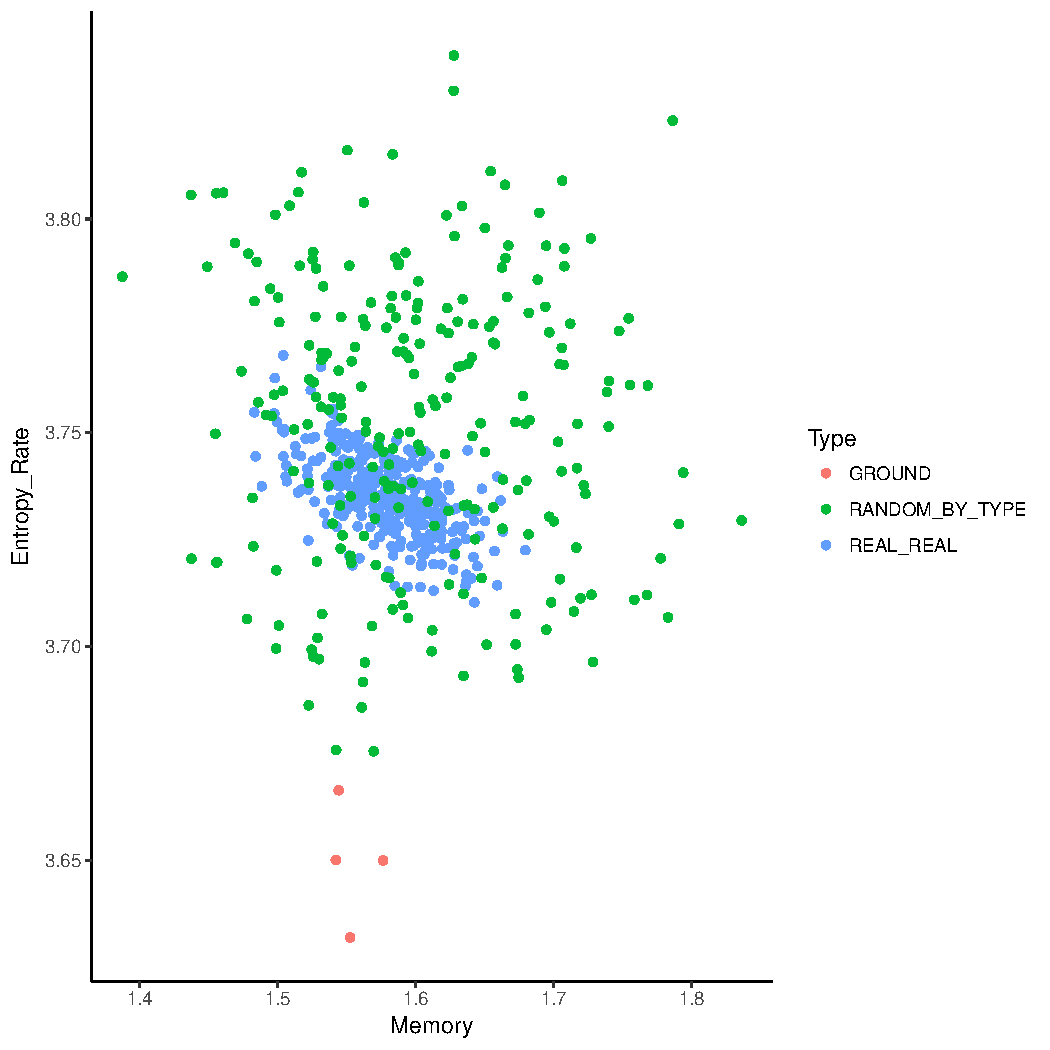
\includegraphics[width=0.25\textwidth]{figures/Estonian-entropy-memory.pdf}}  &  \multirow{4}{*}{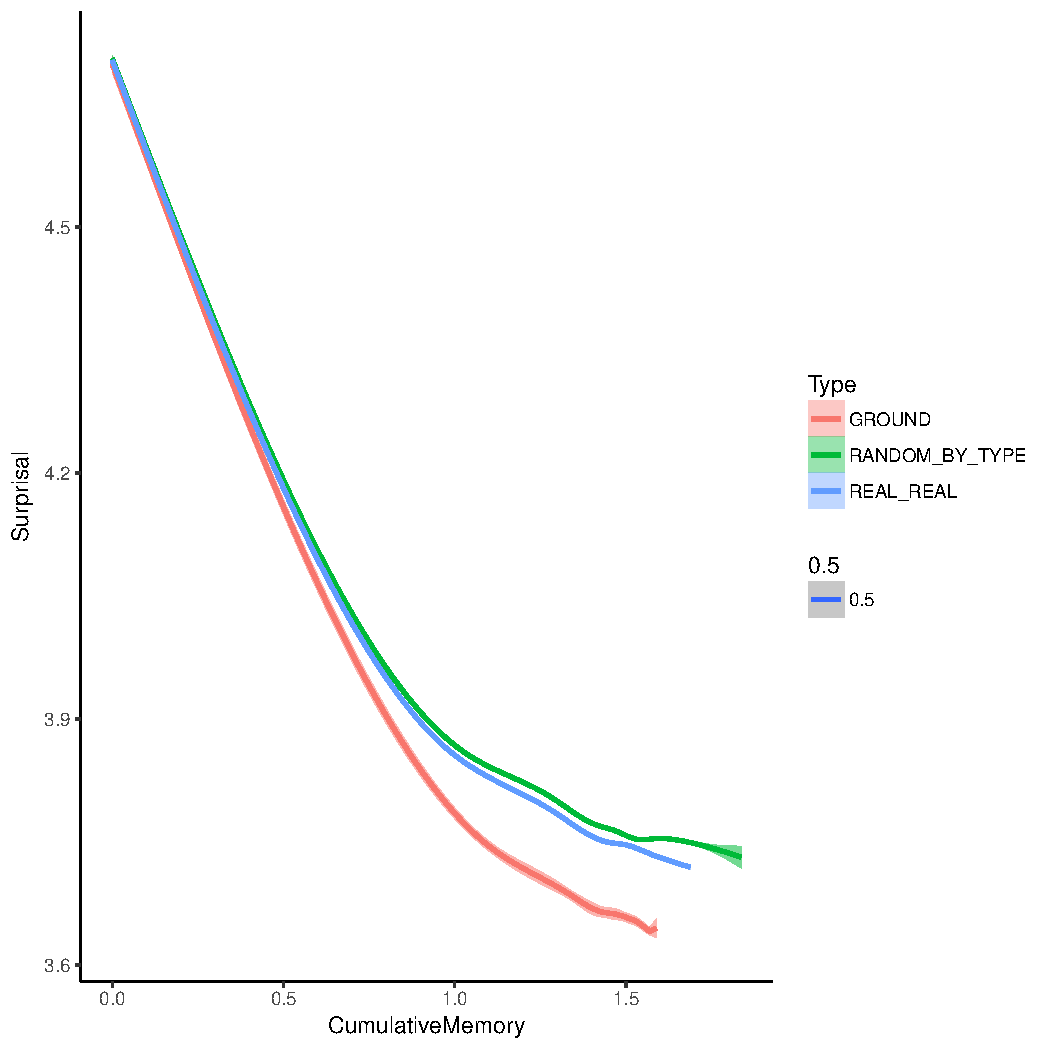
\includegraphics[width=0.25\textwidth]{figures/Estonian-listener-surprisal-memory.pdf}}  &  $D_x$  &  0.39  &  [0.3, 0.48]  \\ 
6959  &    &    &  $B_x-A_x$  &  0.26  &  [0.18, 0.36]  \\ 
  &    &    &  $E_x$  &  0.76  &  [0.67, 0.84]  \\ 
  &    &    &  $W_x$  &  0.72  &  [0.65, 0.79]  \\ [10.25ex] \hline
Faroese-Adap  &  \multirow{4}{*}{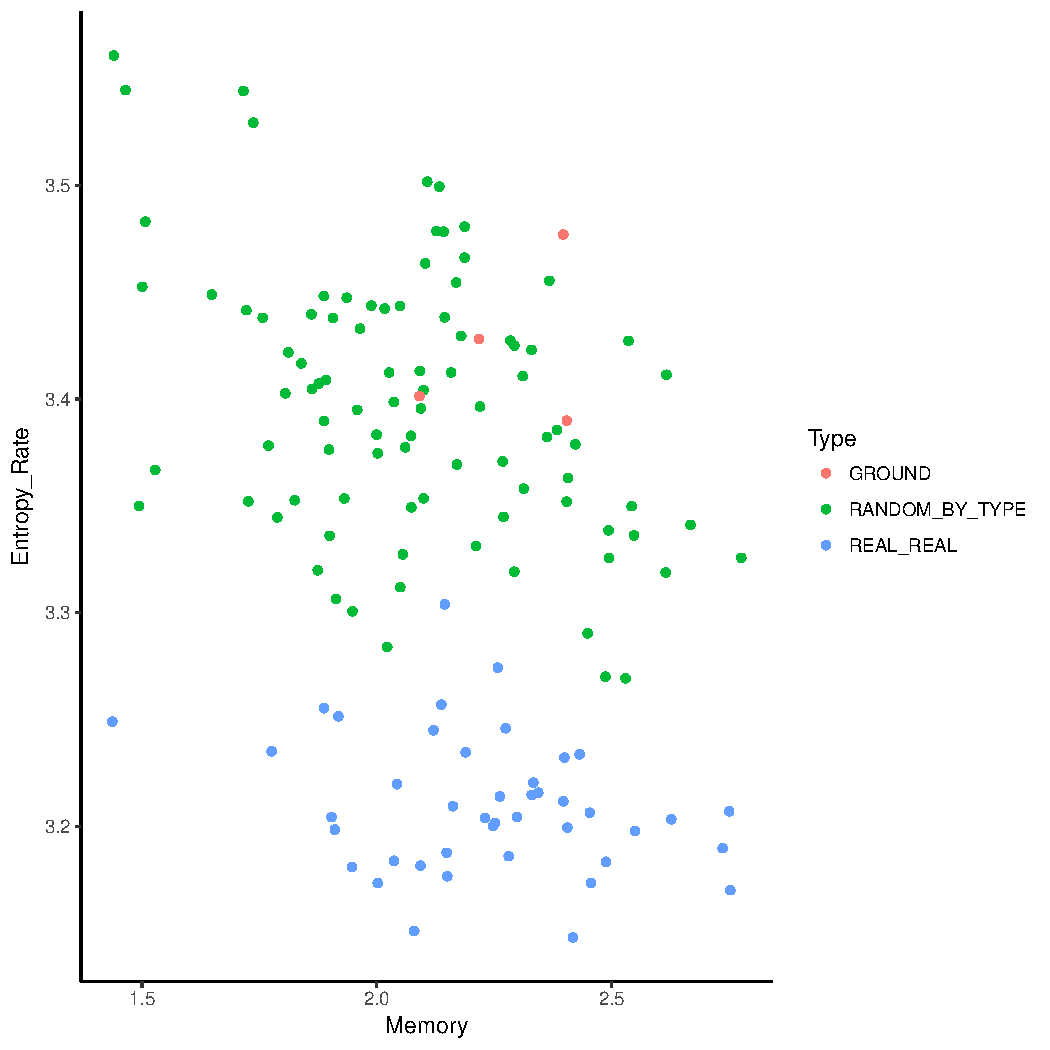
\includegraphics[width=0.25\textwidth]{figures/Faroese-Adap-entropy-memory.pdf}}  &  \multirow{4}{*}{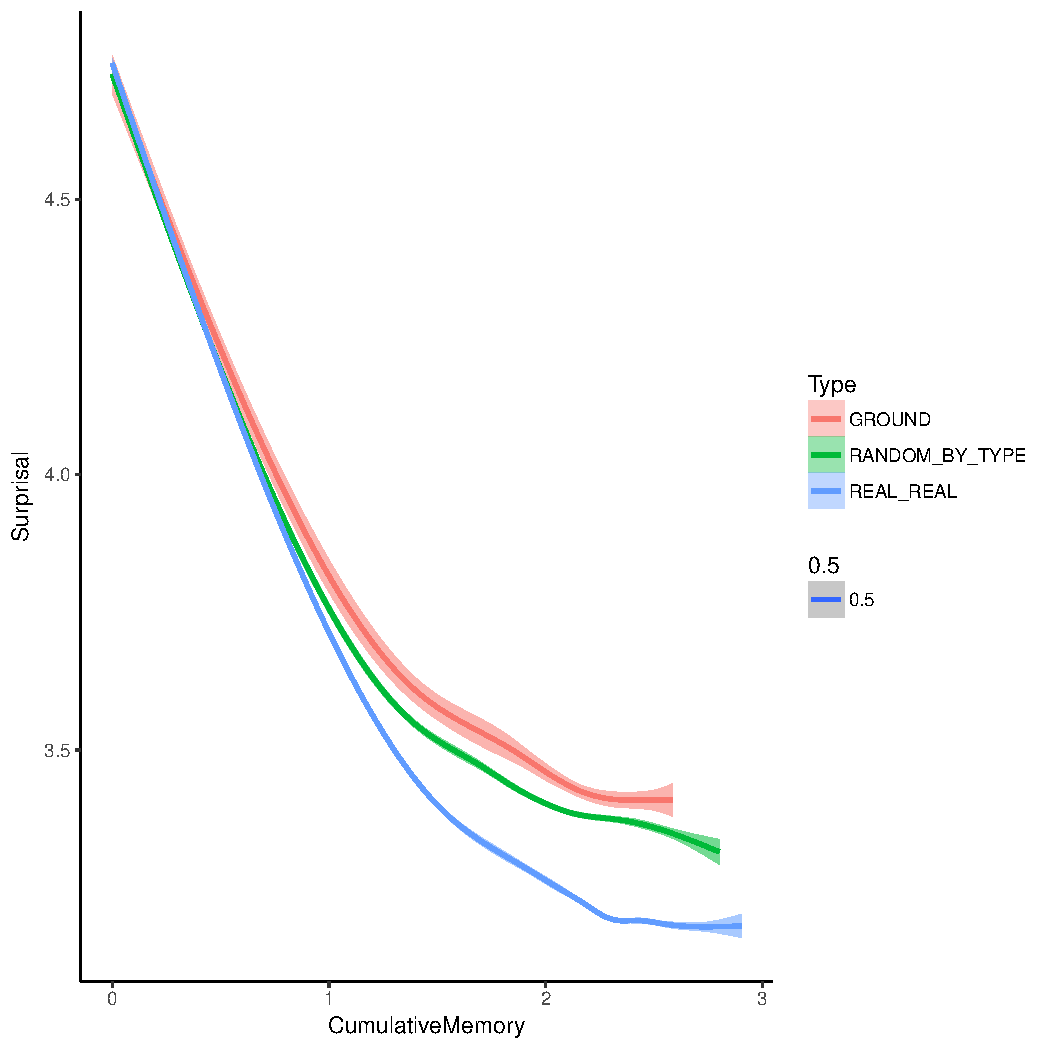
\includegraphics[width=0.25\textwidth]{figures/Faroese-Adap-listener-surprisal-memory.pdf}}  &  $D_x$  &  0.13  &  [0.05, 0.26]  \\ 
1108  &    &    &  $B_x-A_x$  &  0.34  &  [0.24, 0.45]  \\ 
  &    &    &  $E_x$  &  1.0  &  [0.99, 1.0]  \\ 
  &    &    &  $W_x$  &  1.0  &  [1.0, 1.0]  \\ [10.25ex] \hline
Finnish  &  \multirow{4}{*}{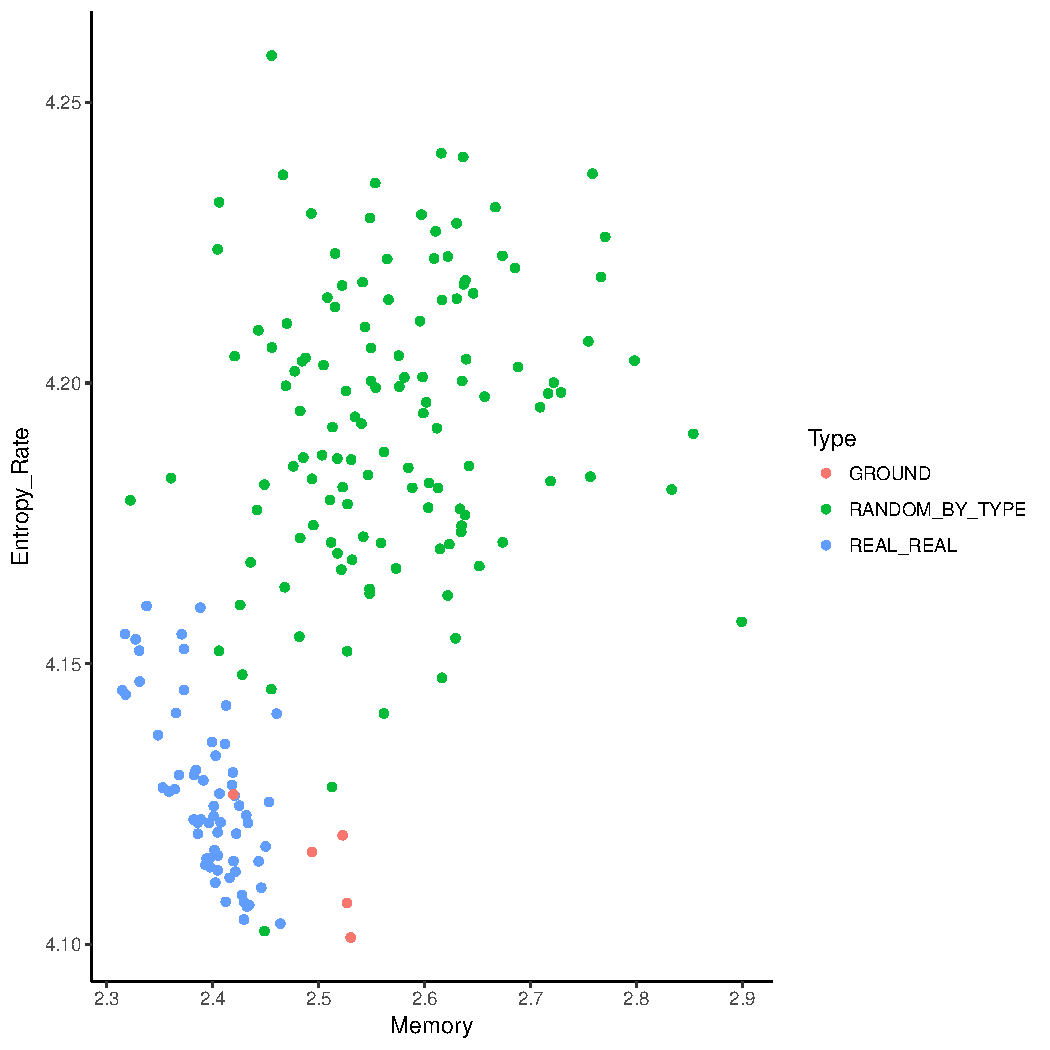
\includegraphics[width=0.25\textwidth]{figures/Finnish-entropy-memory.pdf}}  &  \multirow{4}{*}{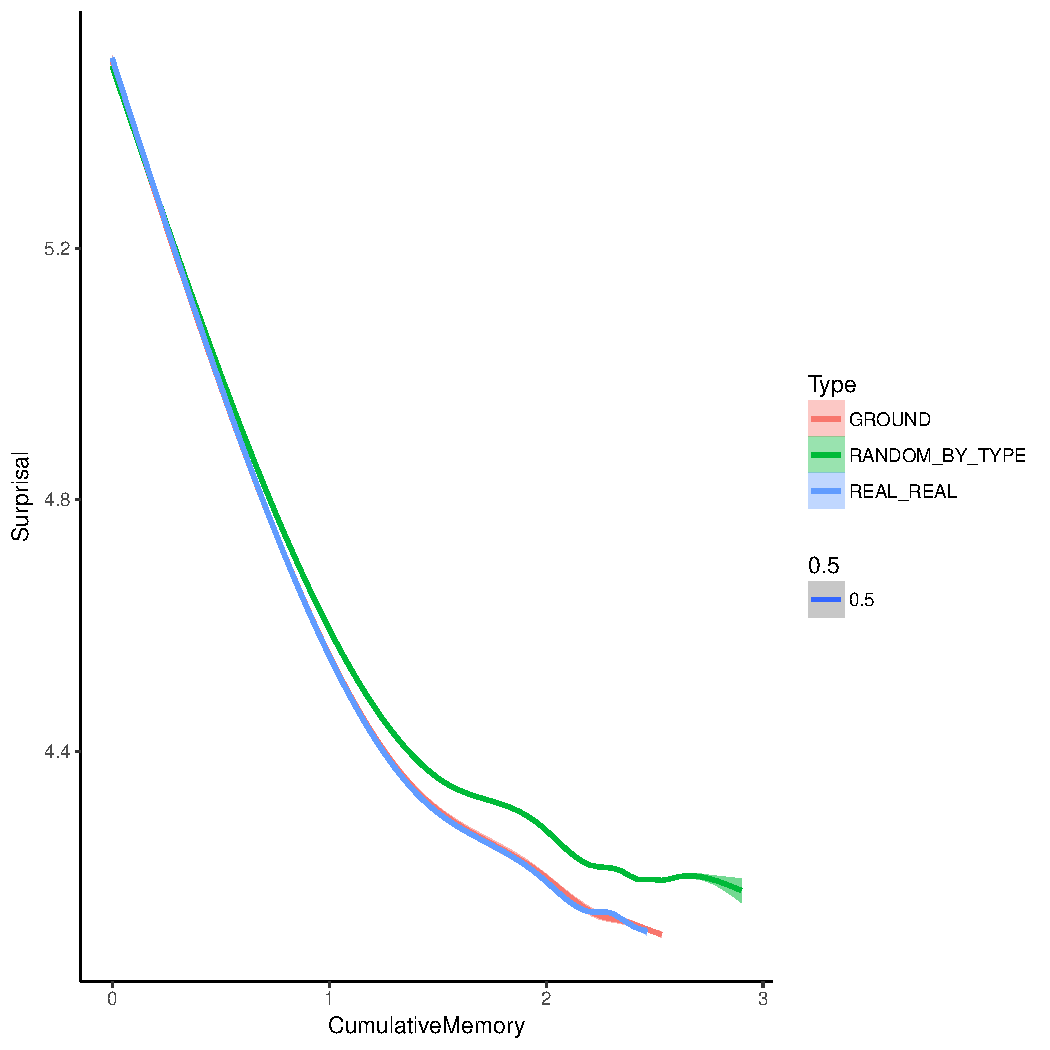
\includegraphics[width=0.25\textwidth]{figures/Finnish-listener-surprisal-memory.pdf}}  &  $D_x$  &  0.05  &  [0.01, 0.12]  \\ 
27198  &    &    &  $B_x-A_x$  &  0.95  &  [0.91, 0.99]  \\ 
  &    &    &  $E_x$  &  1.0  &  [1.0, 1.0]  \\ 
  &    &    &  $W_x$  &  1.0  &  [1.0, 1.0]  \\ [10.25ex] \hline
French*  &\\ [10.25ex] \hline
German  &  \multirow{4}{*}{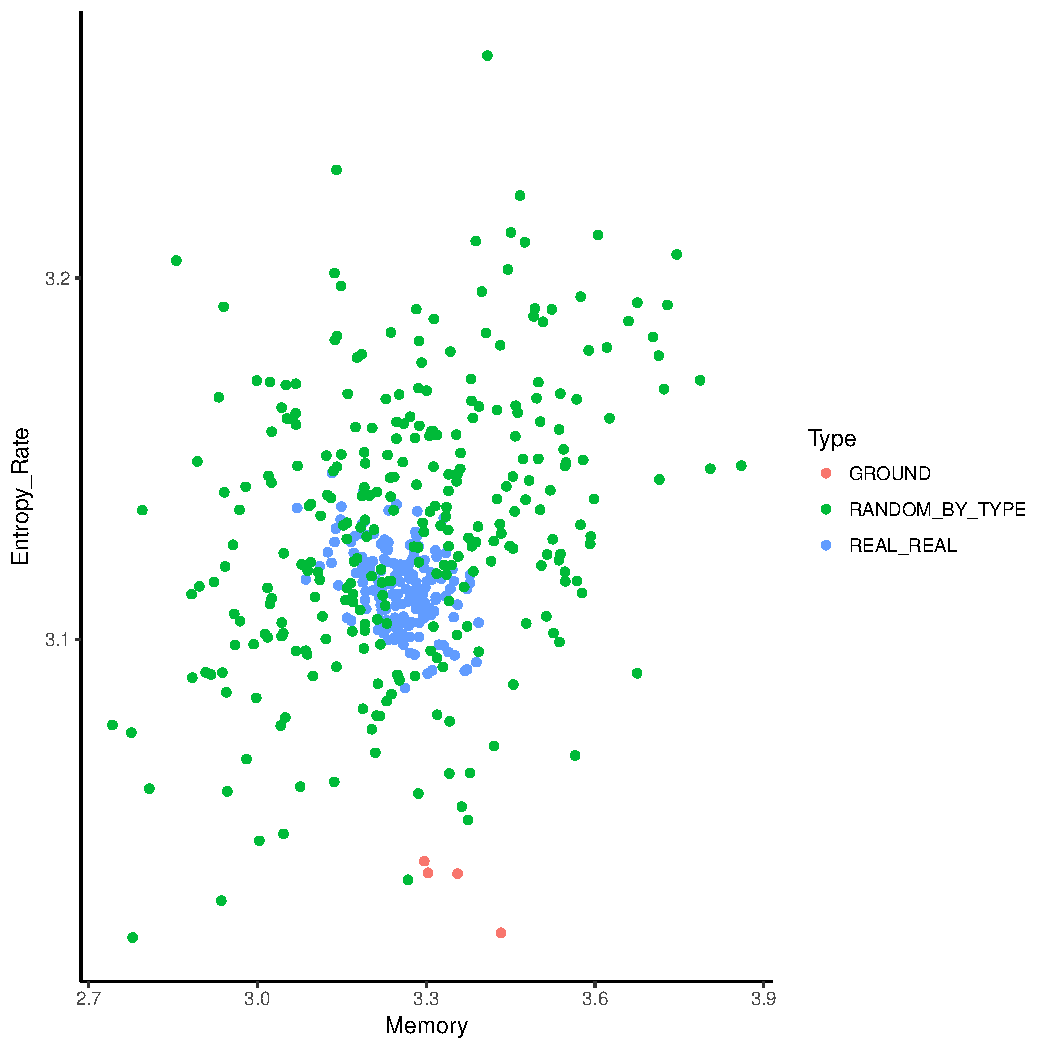
\includegraphics[width=0.25\textwidth]{figures/German-entropy-memory.pdf}}  &  \multirow{4}{*}{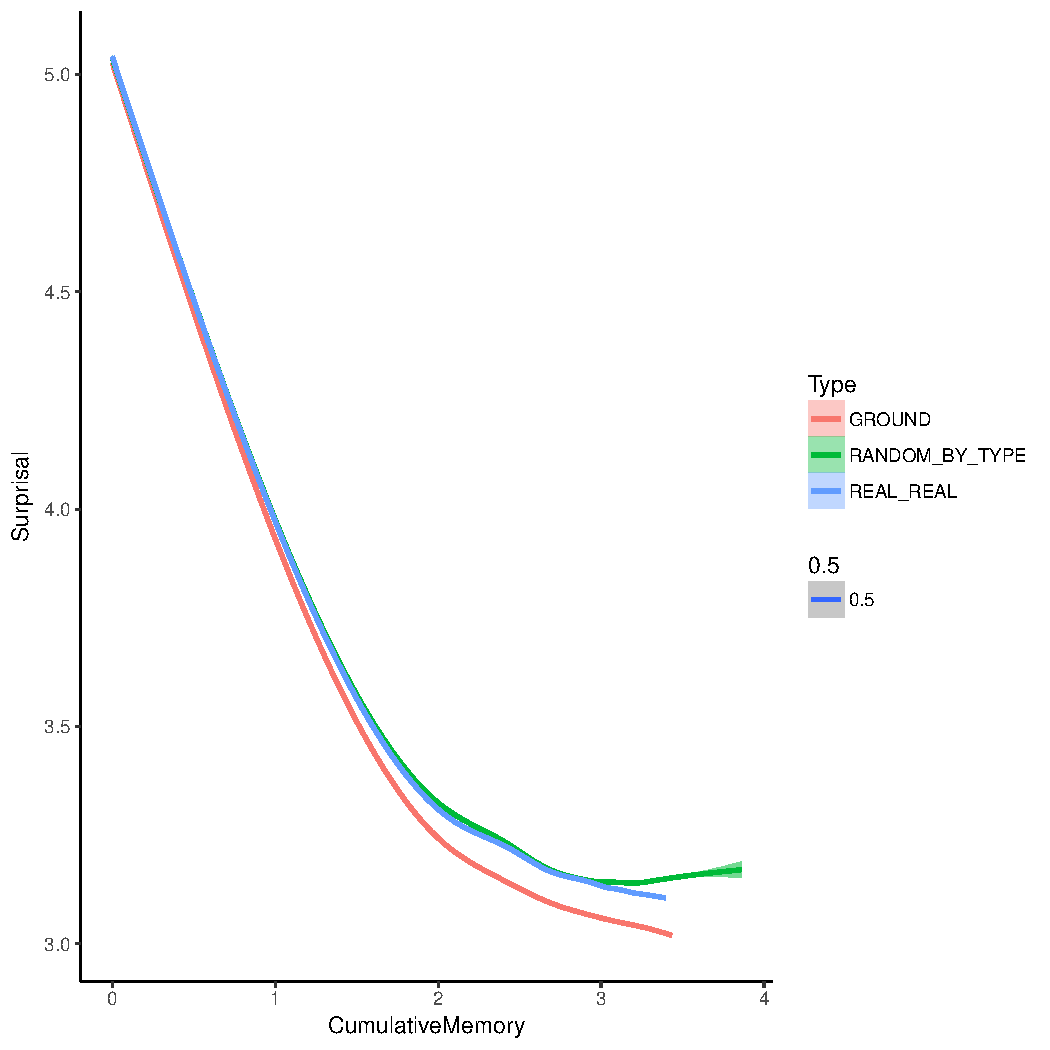
\includegraphics[width=0.25\textwidth]{figures/German-listener-surprisal-memory.pdf}}  &  $D_x$  &  0.44  &  [0.37, 0.51]  \\ 
13814  &    &    &  $B_x-A_x$  &  0.19  &  [0.12, 0.29]  \\ 
  &    &    &  $E_x$  &  0.66  &  [0.6, 0.74]  \\ 
  &    &    &  $W_x$  &  0.63  &  [0.57, 0.69]  \\ [10.25ex] \hline
Greek  &  \multirow{4}{*}{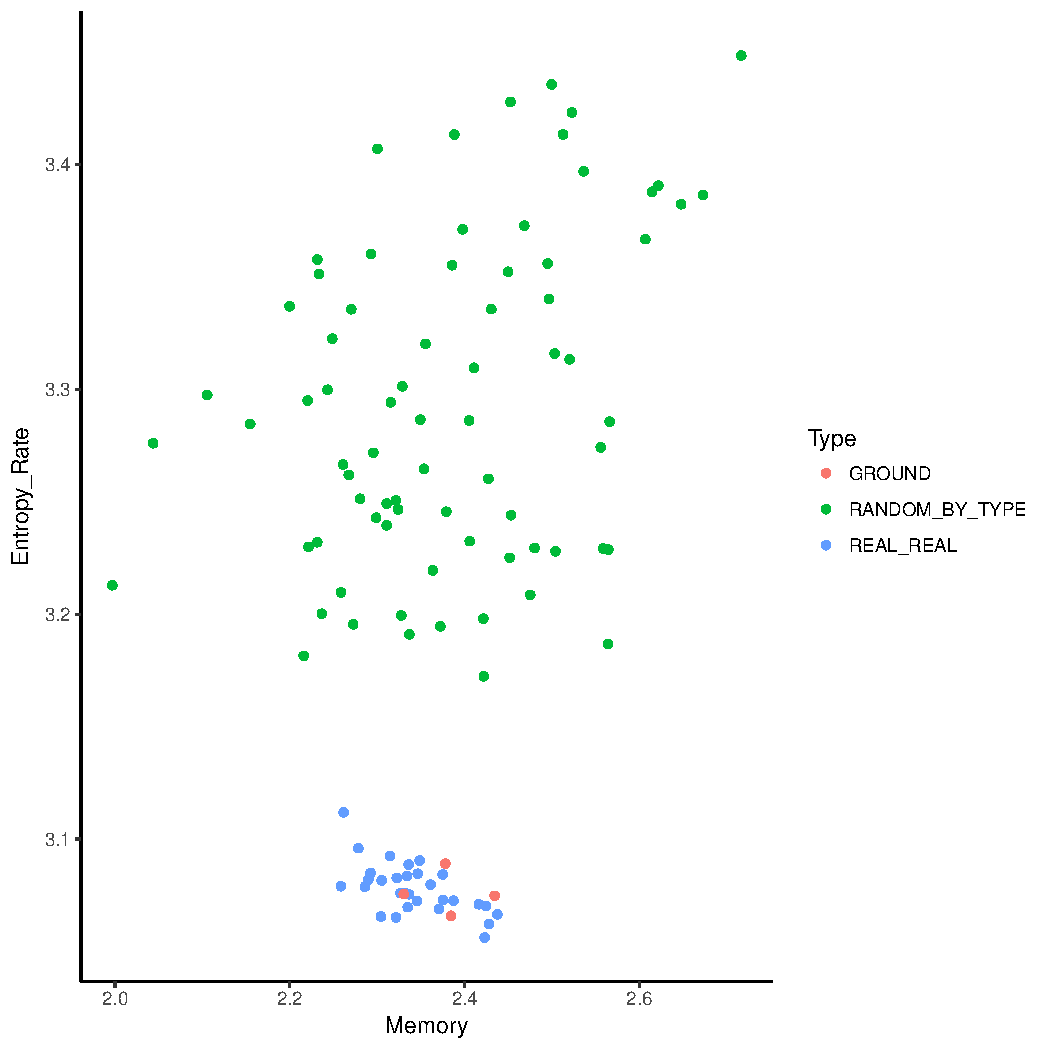
\includegraphics[width=0.25\textwidth]{figures/Greek-entropy-memory.pdf}}  &  \multirow{4}{*}{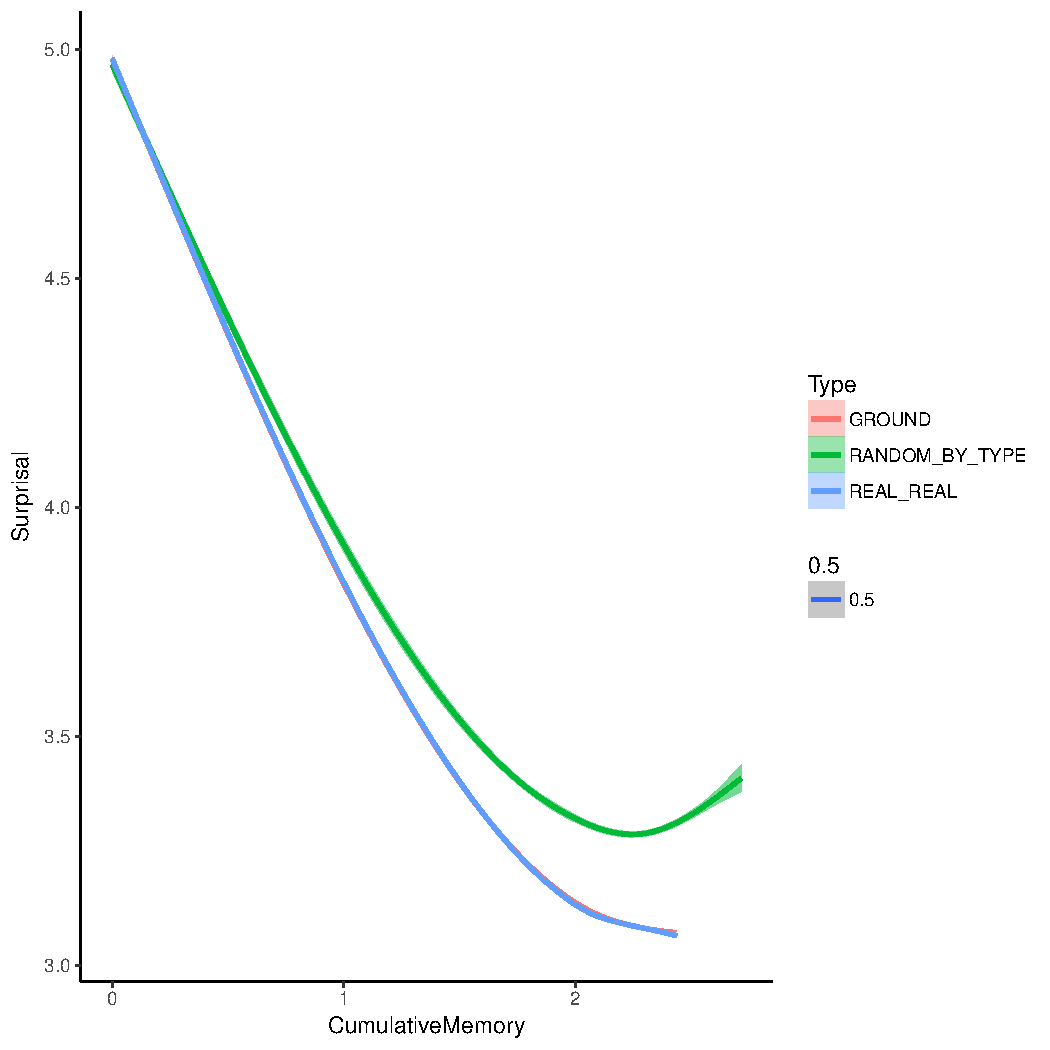
\includegraphics[width=0.25\textwidth]{figures/Greek-listener-surprisal-memory.pdf}}  &  $D_x$  &  0.07  &  [0.0, 0.2]  \\ 
1662  &    &    &  $B_x-A_x$  &  0.59  &  [0.48, 0.73]  \\ 
  &    &    &  $E_x$  &  1.0  &  [1.0, 1.0]  \\ 
  &    &    &  $W_x$  &  1.0  &  [1.0, 1.0]  \\ [10.25ex] \hline
Hebrew  &  \multirow{4}{*}{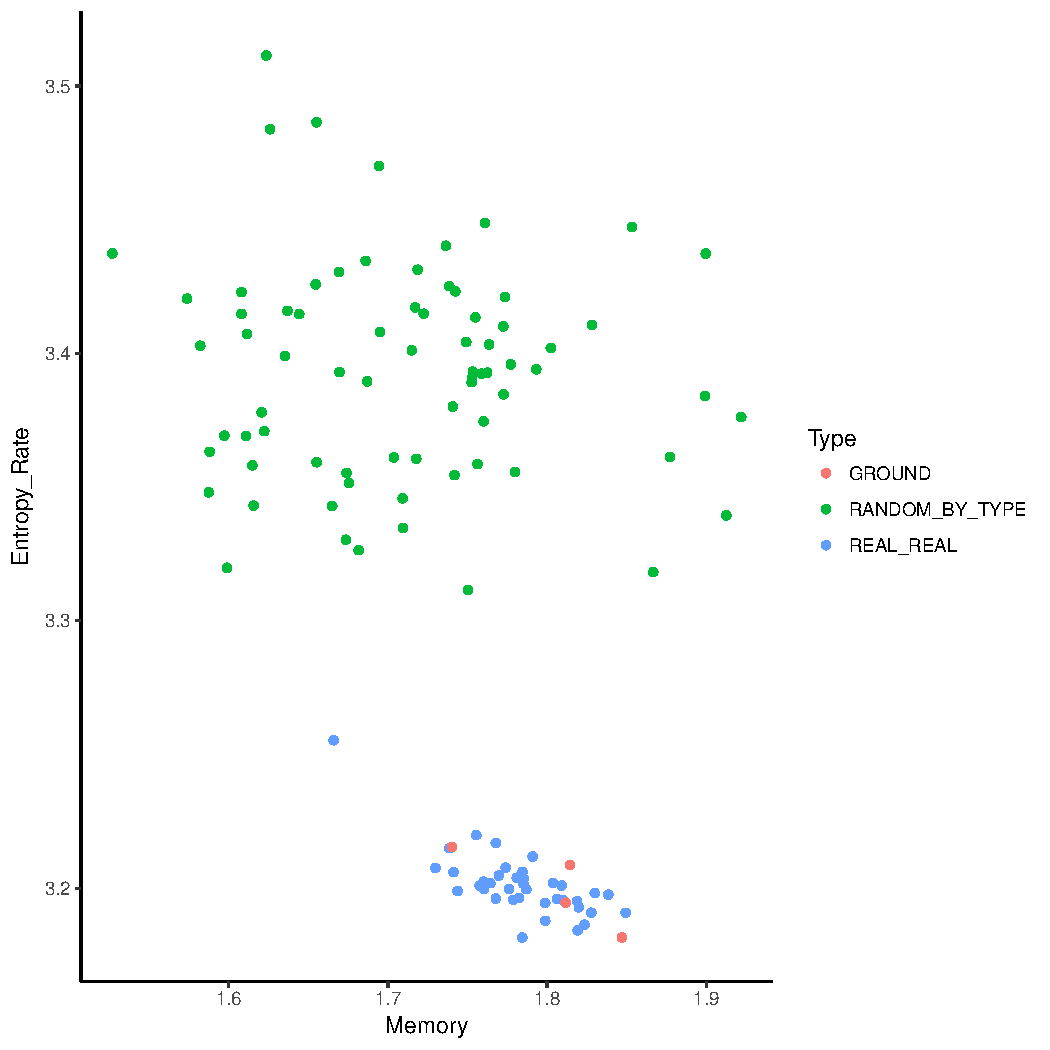
\includegraphics[width=0.25\textwidth]{figures/Hebrew-entropy-memory.pdf}}  &  \multirow{4}{*}{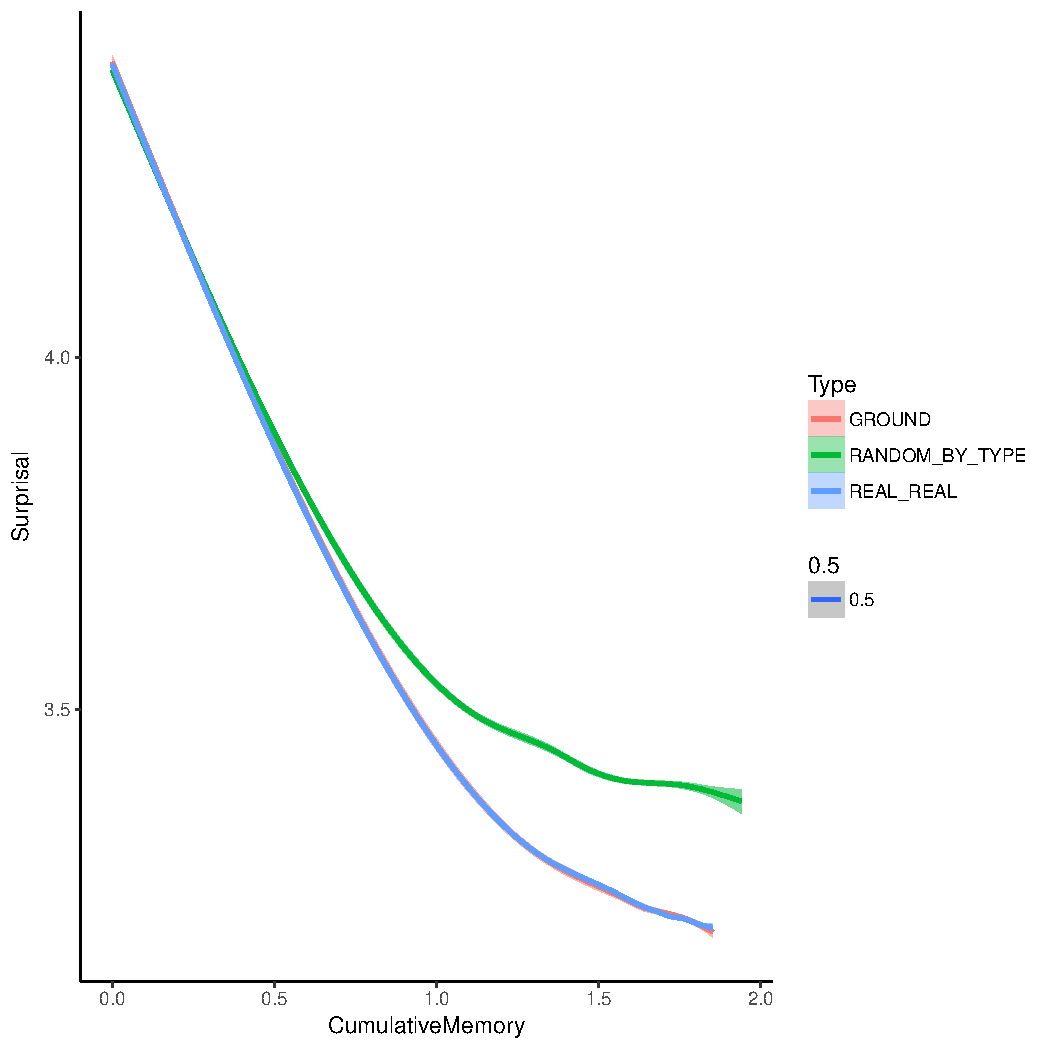
\includegraphics[width=0.25\textwidth]{figures/Hebrew-listener-surprisal-memory.pdf}}  &  $D_x$  &  0.12  &  [0.03, 0.24]  \\ 
5241  &    &    &  $B_x-A_x$  &  0.19  &  [0.08, 0.3]  \\ 
  &    &    &  $E_x$  &  1.0  &  [1.0, 1.0]  \\ 
  &    &    &  $W_x$  &  1.0  &  [1.0, 1.0]  \\ [10.25ex] \hline
Hindi  &  \multirow{4}{*}{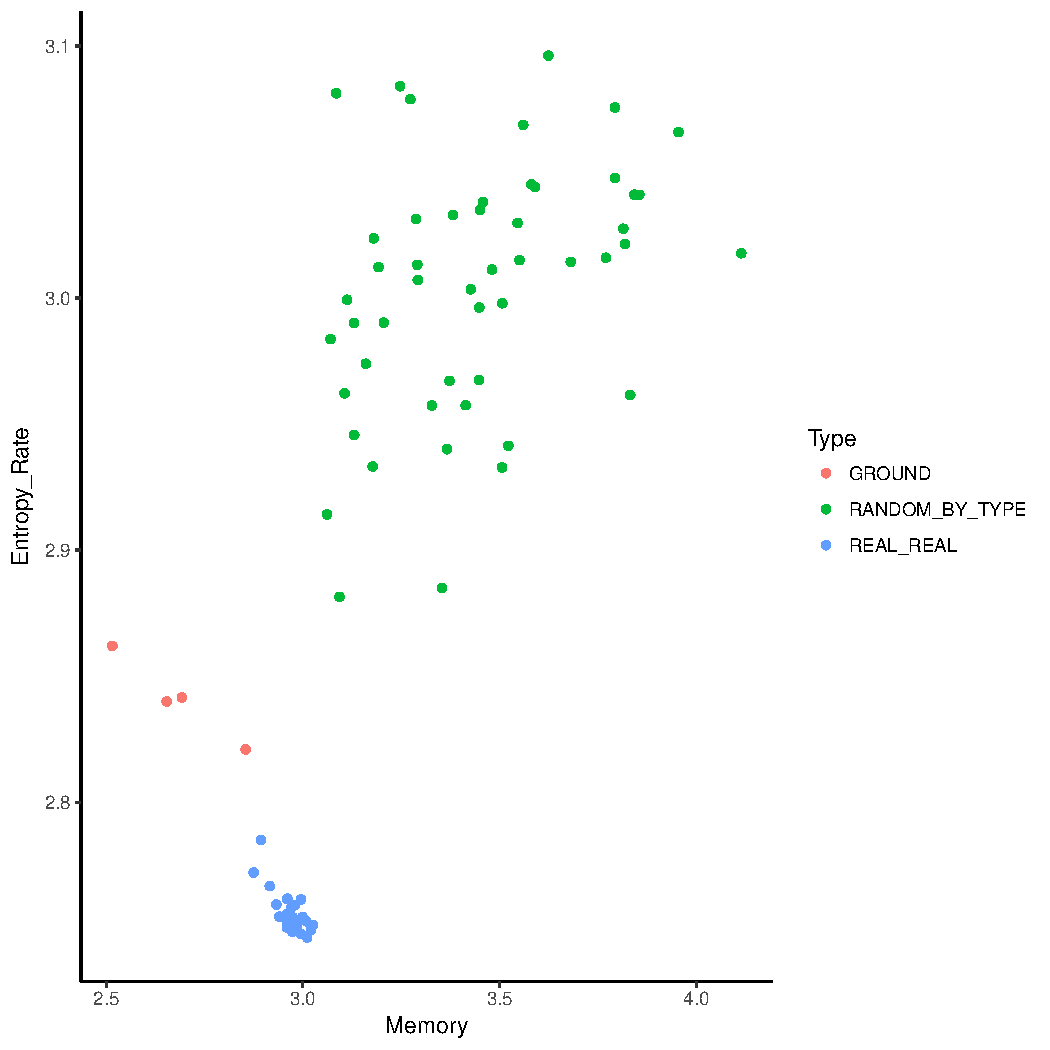
\includegraphics[width=0.25\textwidth]{figures/Hindi-entropy-memory.pdf}}  &  \multirow{4}{*}{\includegraphics[width=0.25\textwidth]{figures/Hindi-listener-surprisal-memory.pdf}}  &  $D_x$  &  0.07  &  [0.0, 0.24]  \\ 
13304  &    &    &  $B_x-A_x$  &  1.0  &  [1.0, 1.0]  \\ 
  &    &    &  $E_x$  &  1.0  &  [1.0, 1.0]  \\ 
  &    &    &  $W_x$  &  1.0  &  [1.0, 1.0]  \\ [10.25ex] \hline
Hungarian  &  \multirow{4}{*}{\includegraphics[width=0.25\textwidth]{figures/Hungarian-entropy-memory.pdf}}  &  \multirow{4}{*}{\includegraphics[width=0.25\textwidth]{figures/Hungarian-listener-surprisal-memory.pdf}}  &  $D_x$  &  0.55  &  [0.44, 0.65]  \\ 
910  &    &    &  $B_x-A_x$  &  0.07  &  [0.0, 0.15]  \\ 
  &    &    &  $E_x$  &  0.62  &  [0.51, 0.74]  \\ 
  &    &    &  $W_x$  &  0.83  &  [0.76, 0.89]  \\ [10.25ex] \hline
Indonesian  &  \multirow{4}{*}{\includegraphics[width=0.25\textwidth]{figures/Indonesian-entropy-memory.pdf}}  &  \multirow{4}{*}{\includegraphics[width=0.25\textwidth]{figures/Indonesian-listener-surprisal-memory.pdf}}  &  $D_x$  &  0.36  &  [0.28, 0.43]  \\ 
4477  &    &    &  $B_x-A_x$  &  0.27  &  [0.22, 0.33]  \\ 
  &    &    &  $E_x$  &  0.82  &  [0.77, 0.87]  \\ 
  &    &    &  $W_x$  &  0.62  &  [0.57, 0.66]  \\ [10.25ex] \hline
Japanese  &  \multirow{4}{*}{\includegraphics[width=0.25\textwidth]{figures/Japanese-entropy-memory.pdf}}  &  \multirow{4}{*}{\includegraphics[width=0.25\textwidth]{figures/Japanese-listener-surprisal-memory.pdf}}  &  $D_x$  &  0.05  &  [0.0, 0.18]  \\ 
7164  &    &    &  $B_x-A_x$  &  1.0  &  [1.0, 1.0]  \\ 
  &    &    &  $E_x$  &  1.0  &  [1.0, 1.0]  \\ 
  &    &    &  $W_x$  &  1.0  &  [1.0, 1.0]  \\ [10.25ex] \hline
Kazakh-Adap  &  \multirow{4}{*}{\includegraphics[width=0.25\textwidth]{figures/Kazakh-Adap-entropy-memory.pdf}}  &  \multirow{4}{*}{\includegraphics[width=0.25\textwidth]{figures/Kazakh-Adap-listener-surprisal-memory.pdf}}  &  $D_x$  &  0.08  &  [0.0, 0.24]  \\ 
947  &    &    &  $B_x-A_x$  &  0.29  &  [0.2, 0.38]  \\ 
  &    &    &  $E_x$  &  1.0  &  [1.0, 1.0]  \\ 
  &    &    &  $W_x$  &  1.0  &  [1.0, 1.0]  \\ [10.25ex] \hline
Kurmanji-Adap  &  \multirow{4}{*}{\includegraphics[width=0.25\textwidth]{figures/Kurmanji-Adap-entropy-memory.pdf}}  &  \multirow{4}{*}{\includegraphics[width=0.25\textwidth]{figures/Kurmanji-Adap-listener-surprisal-memory.pdf}}  &  $D_x$  &  0.21  &  [0.09, 0.36]  \\ 
634  &    &    &  $B_x-A_x$  &  0.1  &  [0.05, 0.16]  \\ 
  &    &    &  $E_x$  &  0.86  &  [0.72, 0.95]  \\ 
  &    &    &  $W_x$  &  0.96  &  [0.92, 1.0]  \\ [10.25ex] \hline
Latvian  &  \multirow{4}{*}{\includegraphics[width=0.25\textwidth]{figures/Latvian-entropy-memory.pdf}}  &  \multirow{4}{*}{\includegraphics[width=0.25\textwidth]{figures/Latvian-listener-surprisal-memory.pdf}}  &  $D_x$  &  0.51  &  [0.41, 0.62]  \\ 
4124  &    &    &  $B_x-A_x$  &  -0.05  &  [-0.11, 0.01]  \\ 
  &    &    &  $E_x$  &  0.37  &  [0.24, 0.53]  \\ 
  &    &    &  $W_x$  &  0.66  &  [0.58, 0.74]  \\ [10.25ex] \hline
Naija-Adap  &  \multirow{4}{*}{\includegraphics[width=0.25\textwidth]{figures/Naija-Adap-entropy-memory.pdf}}  &  \multirow{4}{*}{\includegraphics[width=0.25\textwidth]{figures/Naija-Adap-listener-surprisal-memory.pdf}}  &  $D_x$  &  0.1  &  [0.02, 0.25]  \\ 
848  &    &    &  $B_x-A_x$  &  0.33  &  [0.21, 0.47]  \\ 
  &    &    &  $E_x$  &  1.0  &  [0.99, 1.0]  \\ 
  &    &    &  $W_x$  &  1.0  &  [1.0, 1.0]  \\ [10.25ex] \hline
North Sami  &  \multirow{4}{*}{\includegraphics[width=0.25\textwidth]{figures/North_Sami-entropy-memory.pdf}}  &  \multirow{4}{*}{\includegraphics[width=0.25\textwidth]{figures/North_Sami-listener-surprisal-memory.pdf}}  &  $D_x$  &  0.36  &  [0.28, 0.45]  \\ 
2257  &    &    &  $B_x-A_x$  &  0.15  &  [0.08, 0.23]  \\ 
  &    &    &  $E_x$  &  0.73  &  [0.62, 0.81]  \\ 
  &    &    &  $W_x$  &  0.36  &  [0.28, 0.43]  \\ [10.25ex] \hline
Norwegian  &  \multirow{4}{*}{\includegraphics[width=0.25\textwidth]{figures/Norwegian-entropy-memory.pdf}}  &  \multirow{4}{*}{\includegraphics[width=0.25\textwidth]{figures/Norwegian-listener-surprisal-memory.pdf}}  &  $D_x$  &  0.14  &  [0.04, 0.3]  \\ 
29870  &    &    &  $B_x-A_x$  &  0.63  &  [0.48, 0.78]  \\ 
  &    &    &  $E_x$  &  1.0  &  [1.0, 1.0]  \\ 
  &    &    &  $W_x$  &  1.0  &  [1.0, 1.0]  \\ [10.25ex] \hline
Persian  &  \multirow{4}{*}{\includegraphics[width=0.25\textwidth]{figures/Persian-entropy-memory.pdf}}  &  \multirow{4}{*}{\includegraphics[width=0.25\textwidth]{figures/Persian-listener-surprisal-memory.pdf}}  &  $D_x$  &  0.17  &  [0.07, 0.32]  \\ 
4798  &    &    &  $B_x-A_x$  &  0.12  &  [0.06, 0.2]  \\ 
  &    &    &  $E_x$  &  0.93  &  [0.77, 1.0]  \\ 
  &    &    &  $W_x$  &  1.0  &  [0.99, 1.0]  \\ [10.25ex] \hline
Polish  &  \multirow{4}{*}{\includegraphics[width=0.25\textwidth]{figures/Polish-entropy-memory.pdf}}  &  \multirow{4}{*}{\includegraphics[width=0.25\textwidth]{figures/Polish-listener-surprisal-memory.pdf}}  &  $D_x$  &  0.39  &  [0.3, 0.5]  \\ 
6100  &    &    &  $B_x-A_x$  &  0.08  &  [-0.0, 0.15]  \\ 
  &    &    &  $E_x$  &  0.6  &  [0.5, 0.69]  \\ 
  &    &    &  $W_x$  &  0.31  &  [0.23, 0.39]  \\ [10.25ex] \hline
Romanian  &  \multirow{4}{*}{\includegraphics[width=0.25\textwidth]{figures/Romanian-entropy-memory.pdf}}  &  \multirow{4}{*}{\includegraphics[width=0.25\textwidth]{figures/Romanian-listener-surprisal-memory.pdf}}  &  $D_x$  &  0.12  &  [0.03, 0.24]  \\ 
8664  &    &    &  $B_x-A_x$  &  0.15  &  [0.07, 0.24]  \\ 
  &    &    &  $E_x$  &  1.0  &  [1.0, 1.0]  \\ 
  &    &    &  $W_x$  &  1.0  &  [1.0, 1.0]  \\ [10.25ex] \hline
Serbian  &  \multirow{4}{*}{\includegraphics[width=0.25\textwidth]{figures/Serbian-entropy-memory.pdf}}  &  \multirow{4}{*}{\includegraphics[width=0.25\textwidth]{figures/Serbian-listener-surprisal-memory.pdf}}  &  $D_x$  &  0.06  &  [0.01, 0.15]  \\ 
2935  &    &    &  $B_x-A_x$  &  0.19  &  [0.13, 0.26]  \\ 
  &    &    &  $E_x$  &  1.0  &  [1.0, 1.0]  \\ 
  &    &    &  $W_x$  &  1.0  &  [1.0, 1.0]  \\ [10.25ex] \hline
Slovak  &  \multirow{4}{*}{\includegraphics[width=0.25\textwidth]{figures/Slovak-entropy-memory.pdf}}  &  \multirow{4}{*}{\includegraphics[width=0.25\textwidth]{figures/Slovak-listener-surprisal-memory.pdf}}  &  $D_x$  &  0.21  &  [0.13, 0.3]  \\ 
8483  &    &    &  $B_x-A_x$  &  0.48  &  [0.39, 0.56]  \\ 
  &    &    &  $E_x$  &  0.94  &  [0.9, 0.97]  \\ 
  &    &    &  $W_x$  &  0.89  &  [0.83, 0.94]  \\ [10.25ex] \hline
Slovenian  &  \multirow{4}{*}{\includegraphics[width=0.25\textwidth]{figures/Slovenian-entropy-memory.pdf}}  &  \multirow{4}{*}{\includegraphics[width=0.25\textwidth]{figures/Slovenian-listener-surprisal-memory.pdf}}  &  $D_x$  &  0.31  &  [0.22, 0.39]  \\ 
7532  &    &    &  $B_x-A_x$  &  0.44  &  [0.35, 0.56]  \\ 
  &    &    &  $E_x$  &  0.85  &  [0.79, 0.92]  \\ 
  &    &    &  $W_x$  &  0.79  &  [0.72, 0.85]  \\ [10.25ex] \hline
Spanish* &\\ [10.25ex] \hline
Swedish  &  \multirow{4}{*}{\includegraphics[width=0.25\textwidth]{figures/Swedish-entropy-memory.pdf}}  &  \multirow{4}{*}{\includegraphics[width=0.25\textwidth]{figures/Swedish-listener-surprisal-memory.pdf}}  &  $D_x$  &  0.11  &  [0.02, 0.29]  \\ 
7041  &    &    &  $B_x-A_x$  &  0.06  &  [0.01, 0.12]  \\ 
  &    &    &  $E_x$  &  1.0  &  [1.0, 1.0]  \\ 
  &    &    &  $W_x$  &  1.0  &  [1.0, 1.0]  \\ [10.25ex] \hline
Tamil  &  \multirow{4}{*}{\includegraphics[width=0.25\textwidth]{figures/Tamil-entropy-memory.pdf}}  &  \multirow{4}{*}{\includegraphics[width=0.25\textwidth]{figures/Tamil-listener-surprisal-memory.pdf}}  &  $D_x$  &  0.15  &  [0.04, 0.29]  \\ 
400  &    &    &  $B_x-A_x$  &  0.17  &  [0.1, 0.28]  \\ 
  &    &    &  $E_x$  &  1.0  &  [1.0, 1.0]  \\ 
  &    &    &  $W_x$  &  1.0  &  [1.0, 1.0]  \\ [10.25ex] \hline
Thai-Adap  &  \multirow{4}{*}{\includegraphics[width=0.25\textwidth]{figures/Thai-Adap-entropy-memory.pdf}}  &  \multirow{4}{*}{\includegraphics[width=0.25\textwidth]{figures/Thai-Adap-listener-surprisal-memory.pdf}}  &  $D_x$  &  0.15  &  [0.06, 0.28]  \\ 
900  &    &    &  $B_x-A_x$  &  0.19  &  [0.12, 0.27]  \\ 
  &    &    &  $E_x$  &  0.99  &  [0.97, 1.0]  \\ 
  &    &    &  $W_x$  &  1.0  &  [1.0, 1.0]  \\ [10.25ex] \hline
Turkish  &  \multirow{4}{*}{\includegraphics[width=0.25\textwidth]{figures/Turkish-entropy-memory.pdf}}  &  \multirow{4}{*}{\includegraphics[width=0.25\textwidth]{figures/Turkish-listener-surprisal-memory.pdf}}  &  $D_x$  &  0.18  &  [0.05, 0.35]  \\ 
3685  &    &    &  $B_x-A_x$  &  0.03  &  [0.01, 0.06]  \\ 
  &    &    &  $E_x$  &  1.0  &  [1.0, 1.0]  \\ 
  &    &    &  $W_x$  &  1.0  &  [1.0, 1.0]  \\ [10.25ex] \hline
Ukrainian  &  \multirow{4}{*}{\includegraphics[width=0.25\textwidth]{figures/Ukrainian-entropy-memory.pdf}}  &  \multirow{4}{*}{\includegraphics[width=0.25\textwidth]{figures/Ukrainian-listener-surprisal-memory.pdf}}  &  $D_x$  &  0.12  &  [0.03, 0.22]  \\ 
4506  &    &    &  $B_x-A_x$  &  0.18  &  [0.1, 0.24]  \\ 
  &    &    &  $E_x$  &  0.94  &  [0.87, 1.0]  \\ 
  &    &    &  $W_x$  &  0.99  &  [0.97, 1.0]  \\ [10.25ex] \hline
Uyghur-Adap  &  \multirow{4}{*}{\includegraphics[width=0.25\textwidth]{figures/Uyghur-Adap-entropy-memory.pdf}}  &  \multirow{4}{*}{\includegraphics[width=0.25\textwidth]{figures/Uyghur-Adap-listener-surprisal-memory.pdf}}  &  $D_x$  &  0.17  &  [0.06, 0.3]  \\ 
1656  &    &    &  $B_x-A_x$  &  0.0  &  [-0.0, 0.01]  \\ 
  &    &    &  $E_x$  &  0.9  &  [0.0, 1.0]  \\ 
  &    &    &  $W_x$  &  0.0  &  [0.0, 0.0]  \\ [10.25ex] \hline
Vietnamese* &\\ [10.25ex] \hline
\end{longtable}


\section{Thoughts}
Upper bound: Use $TH[X_t] - \sum_{t=1}^T (T-t) I_t = T (H[X_t] - \sum_{t=1}^T I_t) + \sum_{t=1}^T t I_t$ bits of memory and incur $\sum_{t>T} I_t$ in additioal surprisal. 


\begin{tabular}{cccccccccccccc}
Afrikaans & Amharic & Arabic & Armenian & Basque & Breton & Bulgarian & Buryat \\
\includegraphics[width=0.14\textwidth]{figures/Afrikaans-listener-surprisal-memory.pdf} & \includegraphics[width=0.14\textwidth]{figures/Amharic-Adap-listener-surprisal-memory.pdf} & \includegraphics[width=0.14\textwidth]{figures/Arabic-listener-surprisal-memory.pdf} & \includegraphics[width=0.14\textwidth]{figures/Armenian-Adap-listener-surprisal-memory.pdf} & \includegraphics[width=0.14\textwidth]{figures/Basque-listener-surprisal-memory.pdf} & \includegraphics[width=0.14\textwidth]{figures/Breton-Adap-listener-surprisal-memory.pdf} & \includegraphics[width=0.14\textwidth]{figures/Bulgarian-listener-surprisal-memory.pdf} & \includegraphics[width=0.14\textwidth]{figures/Buryat-Adap-listener-surprisal-memory.pdf}
\\
Cantonese & Catalan & Chinese & Croatian & Czech & Danish & Dutch & Estonian \\
\includegraphics[width=0.14\textwidth]{figures/Cantonese-Adap-listener-surprisal-memory.pdf} & \includegraphics[width=0.14\textwidth]{figures/Catalan-listener-surprisal-memory.pdf} & \includegraphics[width=0.14\textwidth]{figures/Chinese-listener-surprisal-memory.pdf} & \includegraphics[width=0.14\textwidth]{figures/Croatian-listener-surprisal-memory.pdf} & \includegraphics[width=0.14\textwidth]{figures/Czech-listener-surprisal-memory.pdf} & \includegraphics[width=0.14\textwidth]{figures/Danish-listener-surprisal-memory.pdf} & \includegraphics[width=0.14\textwidth]{figures/Dutch-listener-surprisal-memory.pdf} & \includegraphics[width=0.14\textwidth]{figures/Estonian-listener-surprisal-memory.pdf}
\\
Faroese & Finnish & French & German & Greek & Hebrew & Hindi & Hungarian \\
\includegraphics[width=0.14\textwidth]{figures/Faroese-Adap-listener-surprisal-memory.pdf} & \includegraphics[width=0.14\textwidth]{figures/Finnish-listener-surprisal-memory.pdf} & \includegraphics[width=0.14\textwidth]{figures/French-listener-surprisal-memory.pdf} & \includegraphics[width=0.14\textwidth]{figures/German-listener-surprisal-memory.pdf} & \includegraphics[width=0.14\textwidth]{figures/Greek-listener-surprisal-memory.pdf} & \includegraphics[width=0.14\textwidth]{figures/Hebrew-listener-surprisal-memory.pdf} & \includegraphics[width=0.14\textwidth]{figures/Hindi-listener-surprisal-memory.pdf} & \includegraphics[width=0.14\textwidth]{figures/Hungarian-listener-surprisal-memory.pdf}
\\
Indonesian & Japanese & Kazakh & Kurmanji & Latvian & Naija & North Sami & Norwegian \\
\includegraphics[width=0.14\textwidth]{figures/Indonesian-listener-surprisal-memory.pdf} & \includegraphics[width=0.14\textwidth]{figures/Japanese-listener-surprisal-memory.pdf} & \includegraphics[width=0.14\textwidth]{figures/Kazakh-Adap-listener-surprisal-memory.pdf} & \includegraphics[width=0.14\textwidth]{figures/Kurmanji-Adap-listener-surprisal-memory.pdf} & \includegraphics[width=0.14\textwidth]{figures/Latvian-listener-surprisal-memory.pdf} & \includegraphics[width=0.14\textwidth]{figures/Naija-Adap-listener-surprisal-memory.pdf} & \includegraphics[width=0.14\textwidth]{figures/North_Sami-listener-surprisal-memory.pdf} & \includegraphics[width=0.14\textwidth]{figures/Norwegian-listener-surprisal-memory.pdf}
\\
Persian & Polish & Romanian & Serbian & Slovak & Slovenian & Spanish & Swedish \\
\includegraphics[width=0.14\textwidth]{figures/Persian-listener-surprisal-memory.pdf} & \includegraphics[width=0.14\textwidth]{figures/Polish-listener-surprisal-memory.pdf} & \includegraphics[width=0.14\textwidth]{figures/Romanian-listener-surprisal-memory.pdf} & \includegraphics[width=0.14\textwidth]{figures/Serbian-listener-surprisal-memory.pdf} & \includegraphics[width=0.14\textwidth]{figures/Slovak-listener-surprisal-memory.pdf} & \includegraphics[width=0.14\textwidth]{figures/Slovenian-listener-surprisal-memory.pdf} & \includegraphics[width=0.14\textwidth]{figures/Spanish-listener-surprisal-memory.pdf} & \includegraphics[width=0.14\textwidth]{figures/Swedish-listener-surprisal-memory.pdf}
\\
Tamil & Thai & Turkish & Ukrainian & Uyghur & Vietnamese \\
\includegraphics[width=0.14\textwidth]{figures/Tamil-listener-surprisal-memory.pdf} & \includegraphics[width=0.14\textwidth]{figures/Thai-Adap-listener-surprisal-memory.pdf} & \includegraphics[width=0.14\textwidth]{figures/Turkish-listener-surprisal-memory.pdf} & \includegraphics[width=0.14\textwidth]{figures/Ukrainian-listener-surprisal-memory.pdf} & \includegraphics[width=0.14\textwidth]{figures/Uyghur-Adap-listener-surprisal-memory.pdf} & \includegraphics[width=0.14\textwidth]{figures/Vietnamese-listener-surprisal-memory.pdf}
\\\end{tabular}



\end{document}

















\appendix
\section{Bounding Memory in Imperfect Modeling}
We derived the nonlocality $M$ as a lower bound on the memory of a model that does optimally well in predicting the input process.
What happens when we consider imperfect (or near-optimal) prediction -- which may be a more realistic model for human processing?


The goal of this section is to show that $M$ is not just a lower bound on the memory required for perfect modeling, but also can be used to derive lower and upper bounds on imperfect modeling by suboptimal models.
To study imperfect modeling, we think of the process $(X_t)$ as fixed, and of a model as a function $f$ mapping histories $X_{<t}$ to memory representations, and computing a probability distribution over the vocabulary for $X_t$ based on the memory representation $f(X_{<t})$.
The memory representation $f(X_{<t})$ is a random variable whose entropy is the memory cost of the model.
In general, a model could use any mapping from memory states to distributions over the vocabulary to make its predictions.
However, we will focus on Bayes-optimal models, i.e., models that correctly compute the distribution of $X_t$ given the memory representation $f(X_{<t})$.
(Other models would incur even higher average surprisal, without reduction in memory cost.)
The average surprisal experienced by such a model is $H[X_t | f(X_{<t})]$, and is lower bounded by the true surprisal, $H[X_t|X_{<t}]$.

This section provides some results relating the model's memory cost $H[f(X_{<t})]$ to the attained surprisal $H[X_t | f(X_{<t})]$.
%Naturally, we expect that lower surprisal rates will require more memory.

%\subsection{Lower bound on approximation with n-th order Markov models}
%Let us assume that there is some $T$ such that $I_t = 0$ for $t > 0$ (e.g., $T$ is the length of the longest sentence in the corpus).
%We know $\sum_{t>T} I_{t}$ 
%If a Markov model has order $n$

There is a direct and obvious connection between the decay of mutual information and approximation by $n$-th order Markov models:
\begin{proposition}\label{prop:markov}
The Bayes-optimal $n$-th order Markov model will experience average surprisal (that is, cross-entropy) exactly $$H[X_t|X_{<t}] + \sum_{t > n} I[X_t, X_0 | X_{1\dots t-1}]$$
\end{proposition}


In the rest of this section, we think about further bounds for the case when we have information about memory, but not necessarily about the decay of mutual informations or the nature of the approximating model.


\subsection{Lower bound on imperfect approximation} 
Here we lower-bound the surprisal experienced by a model about which we only know that it has memory $J$ less than $M$, and where have no further knowledge about its structure.

As one might hope, models with memory $J$ less than $M$ will necessarily show greater average surprisal than a perfect model (simply because they cannot be perfect models by the previous proposition).
How much greater will their surprisal be? In general, if a model has memory much smaller than $M$, we cannot conclude that it must have very high average surprisal.\footnote{Example: consider, for each $T \in \mathbb{N}$, a process where $I_{T} = 1$, and $I_{t} = 0$ for $t \neq T$. We have $M = T$, but, even as $T \rightarrow \infty$, a model with zero memory achieves a KL loss of only 1. In this case, Proposition \ref{prop:lower-bound} yields the correct result.}
However, we can get such a bound in relation to the contribution of long-term dependencies to $M$.
%The state I've arrived at so far is still a bit complicated, but there is a reasonable final result for a wide class of processes.
%For smaller contribution of long-term dependencies is to $M$, we can lower bound the model's surprisal more strongly.
We write $$I_t := I[X_t, X_0 | X_{1\dots t-1}]$$








The following result holds for any process:
\begin{proposition}[Approximation by Models with Small Memory, lower bound]~\label{prop:lower-bound}
%For any $T \in \mathbb{N}$, a model with memory $J$ will experience average surprisal (that is, cross-entropy) at least $$H[X_t|X_{<t}] + \sum_{t \leq T} \frac{t}{T} I_t + \sum_{t > T} I_t - J/T$$
%Let $\epsilon > 0$, $T \in \mathbb{N}$ such that $\sum_{t > T} t I_t < \epsilon$.
%$$\sum_{t > T} t I[X_t, X_0 | X_{1\dots t-1}] < \epsilon$$
%Then a model with memory $J$ will experience average surprisal (that is, cross-entropy) at least $$H[X_t|X_{<t}] + \frac{M-J-\epsilon}{T} + \sum_{t > T} I_t$$
%Choose any $T \in \mathbb{N}$.
Any model with memory $J$ will experience average surprisal (that is, cross-entropy) at least
$$H[X_t|X_{<t}] +\sup_{T\in \mathbb{N}}\ \left[ \frac{\left(\sum_{t=1}^T t I_t\right)-J}{T} + \sum_{t > T} I_t\right]$$
%$$H[X_t|X_{<t}] + \sup_{T\in \mathbb{N}}\ \left[\frac{M-J}{T} - \sum_{t > T} (t/T - 1) I_t\right]$$
\end{proposition}
%The second term confirms the intuition that the model's surprisal should grow with the difference $M-J$, but the strength of the bound depends on the choice of $T$.\footnote{The bound can be vacuous for small choices of $T$: If we choose $T = 1$, the bound simply evaluates to the trivial lower bound $H[X_t] - J$, which may be even weaker than the likewise trivial lower bound $H[X_t|X_{<t}]$. It will become clear below that the bound is always nonvacuous when $T$ is large enough.}
%An equivalent way of stating this bound is:
Finding the optimal $T$ will require knowledge of the decay profile $I_t.$\footnote{For any fixed $T$, one can find a decay profile for which the bound would end up vacuous at that $T$, but meaningful for a larger $T$.}
Note that this bound only requires knowledge of $J$ and $I_t$, but no further knowledge of the process and the model.
I think that the bound is also optimal among all bounds that only require knowledge of $J$ and $I_t$, in the sense that for every choice of $I_t$ and $J$, there is a process and a model for which the bound is attained.\footnote{There can be no general nonvacuous bound relying only on $M$ and $J$, as shown in a previous footnote.}


\begin{proof}
Let $f$ be the function mapping histories $X_{<t}$ to memory representations of the model. By assumption, $f(X_{<t})$ can be encoded with up to $J$ bits, so $H[f(X_{<t})] \leq J$.
As explained above, without loss of generality, we can assume that the model is Bayes optimal. %: the model's distribution over $X_t$ after reading $X_{<t}$ is equal to $P(X_t | f(X_{<t}))$ (any other model would incur even higher surprisal).
By definition, the difference between the model's surprisal and optimal surprisal is
\footnote{The first inequality seems really crude. In general, we cannot do better. If we know more about the approximating model, we might be able to improve this. Also, consider the relation to the other inequality. Can they be attained at the same time?}
\begin{align*}
%& - \E_{X} \log P(X_t | f(X_{<t})) - \log P(X_t | X_{<t})\ \ \ \ \ \ \text{(for any $t$, due to stationarity)} \\
%& = - \frac{1}{T} \E_{X} \sum_{t=1}^T \log P(X_t | f(X_{<t})) - \log P(X_t | X_{<t}) \\
%& \geq  - \frac{1}{T} \E_{X} \log P(X_{1\dots T} | f(X_{<0})) - \log P(X_{1\dots T} | X_{<0})  \\
& H[X_t | f(X_{<t})] - H[X_t | X_{<t}] =  \frac{1}{T} \sum_{t=1}^{T} \left(H[X_t | f(X_{<t})] - H[X_t | X_{<t}]\right) \\
& \geq   \frac{1}{T} \left(H[X_{1\dots T} | f(X_{\leq 0})] - H[X_{1\dots T} | X_{\leq 0}]\right)  = \frac{1}{T} \left(I[X_{1\dots T}|X_{\leq 0}] - I[X_{1\dots T}|f(X_{\leq 0})]\right) \\
& = \frac{1}{T} \left(\sum_{t \leq T} t I_t + T \sum_{t > T} I_t - I[X_{1\dots T}|f(X_{\leq 0})]\right) = \frac{1}{T} \left(M - \sum_{t > T} t I_t + T \sum_{t > T} I_t - I[X_{1\dots T}|f(X_{\leq 0})]\right) \\
& \geq \frac{1}{T} \left(M + \sum_{t > T} (T-t) I_t - J\right) 
\end{align*}
\end{proof}
%We can restate this bound in the following two, maybe more insightful, ways:\footnote{Note that (1) and (2) make clear that the bound is guaranteed to be larger than the basic bound $H[X_t|X_{<t}]$ when $T$ is chosen sufficiently large, but the gain over that trivial bound diminishes as $T \rightarrow \infty$. Finding an optimal $T$ that makes the bound as large as possible will depend on the process in question.}
%
%\begin{corollary}
%(1) A model with memory $J$ will experience average surprisal at least $$H[X_t|X_{<t}] +\sup_{T\in \mathbb{N}}\ \left[ \frac{\left(\sum_{t=1}^T t I_t\right)-J}{T} + \sum_{t > T} I_t\right]$$
%
%(2) Let $\epsilon > 0$, $T \in \mathbb{N}$ such that $\sum_{t > T} t I_t < \epsilon$.
%Then a model with memory $J$ will experience average surprisal (that is, cross-entropy) at least $$H[X_t|X_{<t}] + \frac{M-J-\epsilon}{T} + \sum_{t > T} I_t$$
%
%\end{corollary}
%
%

Here is way of phrasing the same statement in terms of memory:
\begin{corollary}
Let $\epsilon > 0$. Then it takes at least (and possibly more than) $$\sup_{T \in \mathbb{N}} \left(\sum_{t=1}^T t I_t\right) + T\left(\sum_{t > T} I_t - \epsilon\right)$$ bits of memory to achieve surprisal $\leq H[X_t|X_{<t}] + \epsilon$.
\end{corollary}



\paragraph{Implication 1: Less information locality requires more memory at the same level of prediction error}
Assume $X$ and $Y$ are processes with mutual informations $I_t^X, I_t^Y$, such that they agree on the entropy rate and the unigram entropy.
Assume that $X$ has greater information locality than $Y$ in the (quite strong) sense that, for any $T$, $$\sum_{t>T} I_t^X \leq \sum_{t>T} I_t^Y$$
Then, when fixing $J$, the lower bound on surprisal provided by the proposition is higher in the case of $Y$ than in the case of $X$.
While this does not mean that every such $X$ will require less memory than every such $Y$ (since this is only a lower bound), it does entail an asymptotic version of this:
If we fix $X$ and decrease the information locality of $Y$ indefinitely strongly, $Y$ will ultimately require more memory than $X$, at the same level of experienced surprisal.







\paragraph{Implication 2: With suboptimal memory, no model can do better than a Markov model}
%What is the optimal $T$?
%It turns out that the optimal $T$ 
Searching for the optimal $T$ in the bound, we find:
\begin{corollary}
Consider any memory requirement $J \in [0,M)$.
Let $T$ be the smallest $T \in \{1,2,\dots\}$ such that $$\left(\sum_{t=1}^T t I_t\right) \geq J$$
Informally, we choose $T$ such that a memory capacity of $\approx J$ is sufficient for perfectly modeling all statistical dependencies up to length $T$ when ignoring any longer dependencies.
Then any model with memory $J$ will experience average surprisal at least $$H[X_t|X_{<t}] + \sum_{t > T} I_t$$
That is, it cannot do better than a $T$-th order Markov model.
\end{corollary}
Informally, this means that, irrespective of the architecture of the approximating model, it cannot do better than a model that spends all its capacity on modeling short-range dependencies, and fully ignores long-range ones.

% a $T$-th order Markov

Here is a way of rephrasing this in terms of memory demand:
\begin{corollary}
Let $\epsilon > 0$, then let $T$ be the largest $T$ such that $\sum_{t > T} I_t > \epsilon$. Then it takes at least (and possibly more than) $\left(\sum_{t=1}^T t I_t\right)$ bits of memory to achieve surprisal $\leq H[X_t|X_{<t}] + \epsilon$.
\end{corollary}




%These statements show that the bound on the model's surprisal becomes stronger if $I_t$ decays faster and the convergence of the partial sums $\sum_{t=1}^T t I_t$ to $M$ (as $T \rightarrow \infty$) becomes faster.
%For natural language, where $I_t$ seems to really decay quite rapidly and where (in this work) we're focusing on information within sentences only, we should expect that these bounds would end up reasonably strong.
%
%Do these results agree with the idea of information locality decreasing memory load?
%%If we consider two processes with the same entropy rate and unigram entropy, but where $I_t$ decays strictly faster for one than the other, then for any $T$, the bound will be greater for the process that has less information locality -- confirming that processes with less information locality require more memory in approximation (TODO work out):
%Assume $X$ and $Y$ are processes with mutual informations $I_t^X, I_t^Y$, such that they agree on the entropy rate and the unigram entropy.
%Assume that $X$ has greater information locality than $Y$ in the (quite strong) sense that, for any $T$, $$\sum_{t>T} I_t^X \leq \sum_{t>T} I_t^Y$$
%Then the lower bound that we derived for surprisal of a model with memory $J$ is stronger (higher) for the process $Y$ that has less information locality.\footnote{Because this is true for any $T$, and thus also for the supremum over all $T$'s.}
%Thus, at least broadly speaking, processes with more information locality can be modeled with lower loss at the same memory cost.
%

\begin{example}
%It follows instantly from the bounds that, if $I_t$ is zero for $t > T$ (i.e., the process is $T$-order Markov), average surprisal of the model is lower-bounded by $H[X_t|X_{<t}] + \frac{M-J}{T}$.\footnote{I think that this bound is optimal: If all we require about $I_t$ is that it is zero for $t > T$, and have no other knowledge about $I_t$, then this bound should be attained by some processes where $I_T = M/T$, and all other $I_t$'s are zero.}
%
Let us consider a class of processes that might be a reasonable model of language: Assume $I_t = \alpha t^{-\beta}$ for some $\alpha > 0$, $\beta >2$ (for smaller $\beta$, we would have $M = +\infty$).
We can bound $M = \sum_{t=1}^\infty \alpha t^{-\beta+1} \geq \int_1^\infty \alpha t^{-\beta+1} dt = \frac{\alpha}{\beta-2}$, and similarly $M \leq \alpha + \frac{\alpha}{\beta-2} = \alpha \frac{\beta-1}{\beta-2}$.

Then we can lower-bound the surprisal of a model with memory $J$ by $H[X_t|X_{<t}]$ plus (TODO algebra errors may lie ahead)
$$\frac{1}{T} \int_1^T \alpha t^{-\beta+1} dt - j/T + \int_T^\infty \alpha t^{-\beta} = T^{-1}[\frac{\alpha}{\beta-2} - J] + T^{-\beta+1} [ \frac{\alpha}{\beta-1} - \frac{\alpha}{\beta-2}]$$
To get an optimal $T$, we can take derivatives and maximize this expression, which gives us (assuming that $[\frac{\alpha}{\beta-2} - J] > 0$, otherwise the maximum will be assumed at $T=1$?)
$$T := \left(\frac{(1-\beta)[ \frac{\alpha}{\beta-1} - \frac{\alpha}{\beta-2}]}{[\frac{\alpha}{\beta-2} - J]}\right)^{1/(\beta-2)}$$
and, plugging back into the bound, get that the model's surprisal is at least
$$ H[X_t|X_{<t}] + \frac{[\frac{\alpha}{\beta-2} - J]^{\frac{\beta-1}{\beta-2}}}{\left((1-\beta) [ \frac{\alpha}{\beta-1} - \frac{\alpha}{\beta-2}]\right)^{1/(\beta-2)}} + \frac{[\frac{\alpha}{\beta-2} - J]^{\frac{\beta+1}{\beta-2}}}{(\beta-1)^{\frac{\beta+1}{\beta-2}} [ \frac{\alpha}{\beta-2} - \frac{\alpha}{\beta-1}]^{\frac{\beta+1}{\beta-2}-1}}$$
which grows monotonically, with slightly superlinear speed, as the approximating model's memory $J$ decreases.
Furthermore, if information locality in the process decreases -- that is, $\beta$ decreases but we adjust $\alpha$ to keep $I[X_t|X_{<t}]$ constant -- it seems that the factor $(\beta-1)$ in both denominators will increase the bound, confirming the intuition that approximating a process with less information locality will require more memory.
\end{example}



%Informally, the reason for this phenomenon is that large values of $M$ could reflect large amounts of information at a small distance, but also small amoutns 

%\begin{corollary}[Approximation by N-Gram Models, lower bound]
%Let $\epsilon > 0$, $ \in \mathbb{N}$ such that $\sum_{t > T} t I_t/P < \epsilon$.
%Then
%$$\frac{\sum_{M/P < t < T} I_t}{P} \geq $$
%
%Any $n$-gram model will experience average surprisal (that is, cross-entropy) $$H[X_t|X_{<t}] + \sum_{t > n} I_t$$
%\end{corollary}
%
%\begin{proof}
%
%\end{proof}
%
%


\subsection{Upper Bounds on imperfect approximation}
$M$ is only a lower bound on memory need, not necessarily identical to it: When we require that the model can optimally model the data, then there are examples where the memory need is much larger than $M$, as proved by~\cite[Section 6]{harsha-communication-nodate} (though it's not clear to me whether they are relevant to language).\footnote{Here is a much simpler example sufficient for our need: Let $Z$ be some random variable with nonzero, finite entropy. Let $Z'$ be an independent copy of $Z$, and let $B \sim Bernoulli(p)$. Then define $(X,Y) := (Z,Z)$ if $B=1$ and $(Z, Z')$ else. We consider the problem of coding $X$ with small memory to predict $Y$ optimally. We have $I[X,Y] = pH[Z]$, but any method of predicting $Y$ from a (possibly randomized) function $f(X)$ of $X$ will be suboptimal unless $H[f(X)] \geq H[X]$. In particular, as $p$ can be made small and $H[Z]$ can be made large, the gap between $I[X,Y]$ and the entropy of any mediating storage representation $f(X)$ can be arbitrarily large. The situation changes when encoding and decoding can share a random string (this randomness is then also averaged over when computing the KL-loss), as shown by \cite{harsha-communication-nodate}, but this doesn't seem to model the setting we're interested in.}

However, this needn't be a problem: As long as we only require \emph{near}-optimal prediction and work in the setting of \emph{sequence prediction}, memory need can be bounded in a way that grows linearly in $M$.
We do this using a result of~\cite{sharan-prediction-2016} showing that the loss of $n$-th order Markov models can be bounded in terms of $M$, and noting that we can compute the storage cost of $n$-th order Markov models.


%By a theorem of (CITE), lower excess entropy translates into better approximation by modeling with fixed context window (n-gram models).

\begin{proposition}[Approximation by Markov Models, upper bound. \cite{sharan-prediction-2016}]
The Bayes-optimal $n$-th order Markov model achieves average surprisal $\leq H[X_t|X_{<t}] + M/n$.
%For any $\epsilon > 0$, an $M/\epsilon$-order Markov model can achieve KL loss $\leq \epsilon$.
\end{proposition}
\begin{proof}
In their Proposition 1, they showed that, for any $\epsilon > 0$, a $M/\epsilon$-order Markov model achieves KL loss $\leq \epsilon$, which gives our statement by rearranging.
(Their result follows directly from Proposition~\ref{prop:markov}, which is also how they prove it.)
\end{proof}
%Compared with the lower bound from the previous section, we see:
Computing the memory cost of a an n-th order Markov model, we can conclude:
\begin{corollary}
(1) For any $\epsilon > 0$, there is a model achieving surprisal $H[X_t|X_{<t}] + \epsilon$ using $\leq M \frac{H[X]}{\epsilon}$ bits of memory.

(2) For any $J < M$, there is a model with memory $J$ that achieves average surprisal at most $$H[X_t|X_{<t}] + \frac{M}{J} H[X_t]$$

\end{corollary}
\begin{proof}
By the proposition, we can achieve a surprisal of $H[X_t|X_{<t}] + \epsilon$ with an $M/\epsilon$-gram model.
This model can be implemented using 
$H[X_1 ... X_{M/\epsilon}] \leq M \frac{H[X]}{\epsilon}$ bits of memory.\footnote{
This bound is really crude. We can compute
\begin{align*}
H[X_1 ... X_{M/\epsilon}] &= \frac{M}{\epsilon} H[X] - \sum_{t=1}^{M/\epsilon} (M/\epsilon-t) I_t
%&= I/\epsilon H[X] - I/\epsilon \left(\sum_{t=1}^{I/\epsilon} I_t\right) + \sum_{t=1}^{I/\epsilon} t I_t \\
%&\leq I/\epsilon H[X] + I \\
%& = I(1+H[X]/\epsilon) \\
\end{align*}
but does this gives us anything?}
The second statement is a rephrasing of the first.
\end{proof}
As expected, this bound on surprisal increases as the available memory $J$ decreases in relation to $M$.
In the case of natural language, $H[X]$ is a reasonably small constant.

%Combining with (REF), we can characterize the surprisal of an $n$-gram model in terms of $M$ as
%\begin{corollary}[Approximation by $n$-gram models]
%The average surprisal $S_n$ of the Bayes-optimal $n$-gram model is bounded as
%$$H[X_t|X_{<t}] + \frac{M}{n} - \left(\sum_{t > n} (t/n - 1) I_t\right)\ \leq\ S_n\ \leq\ H[X_t|X_{<t}] + \frac{M}{n}$$
%\end{corollary}




%\subsection{Summary}

%
%\paragraph{Invariance properties under certain transformations of the sequence}
%%Because $I$ is the mutual information between past and future observations, it is invariant under various transformations of the sequence:
%%First, if, say a filler word is randomly added into places in the sequence, the entropy rate will increase but $I$ will stay the same.
%%Second, 
%If we split tokens (deterministically and invertibly) into subtokens, but only measure the memory that is transmitted across the boundaries that were token boundaries before this transformation, $I$ will stay the same.
%If we measure memory also at all new boundaries, $I$ can at most increase.
%On the other hand, if we merge tokens (deterministically and invertibly), $I$ can at most decrease.
%
%%These invariance properties are remarkable since $I$, at the same time, is a measure of the \emph{locality} of information and the \emph{decay} of mutual information over distances.
%


\section{Crypticity}


%We let $X_t$ be a process of observations (e.g. words), and $M_t$ be the internal memory states of the listener, which we can take to be a function of $X_{\leq t}$.
Under the assumption of optimality oif predictions and minimality of memory cost, we can take $M_t$ to be an equivalence class of pasts that induce the same distribution over futures (need to be careful for general processes. we here want to add the assumption that, since we are interested in sentence processing, memory is reset entirely at sentence or discourse boundaries, avoiding cases where the math wouldn't work so nicely).

Nonlocality:
\begin{equation}\label{eq:locality-cost}
L := \sum_{t=1}^\infty\ t \cdot \operatorname{I}[X_t, X_0 | X_1, ..., X_{t-1}]
\end{equation}

Crypticity:
\begin{equation}\label{eq:ambiguity-cost}
A := H[M_0|X_{> 0}]
\end{equation}


Note that both terms are nonnegative by definition.



\begin{proof}
By the definitions of conditional entropy and mutual information,
$H[M_0] = H[M_0 | X_{>0}] + I[M_0, X_{>0}]$
The first part is Ambiguity cost.
Now we show that the second part is equal to Locality cost.
As we assume that the listeners predictions are optimal, $I[M_0, X_{>0}] = I[X_{\leq 0}, X_{>0}]$.
Then the formula is a consequence of the chain rule for mutual information:
\begin{align*}
I[(X_i)_{i > 0}, (X_i)_{i \leq 0}] &= \sum_{i=1}^\infty I(X_i, (X_i)_{i \leq 0}|X_1, ..., X_{i-1}) \\
&= \sum_{i=1}^\infty \sum_{j=0}^{-\infty} I(X_i, X_j|X_{j+1}...X_{i-1}) \\
& = \sum_{t=1}^\infty\ t \cdot \operatorname{I}[X_t, X_0 | X_1, ..., X_{t-1}]
\end{align*}
\end{proof}





\end{document}








\section{Normalized Excess Entropy}

We quantify information (non-)locality by $\frac{I[X_{\geq t}, X_{<t}]}{I[X_t, X_{<t}]}$

Why?

(1) The memory bound is then exactly the amount of information that needs to be transmitted from the past for one word times this quantity

(2) In the plot of decay of MIs, this is the center of mass: At what distance is the predictive information about the current word stored on average?









\section{Computing a tighter lower bound}

Here is a method that takes a quadratic amount of time to compute:

Take all pairs of positions in the corpus, and for each pair $s, t$ compute
$$P(X_{t, ..., t+T}|T_{s-T, ..., s-1})$$
After fixing $\epsilon > 0$, find a partitioning $\Pi$ of the positions $T, ..., N-T$ ($N$ corpus length) such that
$$\frac{1}{N-2T} \sum_{t=T}{N-T} \left( - \log \frac{1}{|\Pi(t)|} \sum_{s \in \Pi(t)} P(X_{t, ..., t+T}|T_{s-T, ..., s-1}) + \log P(X_{t, ..., t+T}|T_{t-T, ..., t-1})\right) < \epsilon$$
Taking the minimum entropy of any such $P$ should be a consistent (as $T$ and the data go to infinity, assuming that the model is already correct, or converges sufficiently strongly) lower bound of memory for modeling with KL loss $\epsilon$.
However, this bound might still not be tight, unless we require that $\Pi(s+1)$ is determined by $\Pi(s)$ and $X_{s+1}$.

Unlike excess entropy, it is not left-right invariant (which is good, because memory is not left-right invariant).

It should be feasible to apply this to POS-level language modeling.



ACTUALLY

Take all pairs of positions in the corpus, and for each pair $s, t$ compute
$$P(X_{t}|T_{s-T, ..., s-1})$$
After fixing $\epsilon > 0$, find a partitioning $\Pi$ of the positions $T, ..., N-T$ ($N$ corpus length) such that
$$\frac{1}{N-2T} \sum_{t=T}{N-T} \left( - \log \frac{1}{|\Pi(t)|} \sum_{s \in \Pi(t)} P(X_{t}|T_{s-T, ..., s-1}) + \log P(X_{t}|T_{t-T, ..., t-1})\right) < \epsilon$$
and
$\Pi(s+1)$ is determined by $\Pi(s)$ and $X_{s+1}$
Taking the minimum entropy of any such $P$ should be a consistent (as $T$ and the data go to infinity, assuming that the model is already correct, or converges sufficiently strongly) estimator of a tight lower bound of memory for modeling with KL loss $\epsilon$.

Unlike excess entropy, it is not left-right invariant (which is good, because memory is not left-right invariant).

It should be feasible to apply this to POS-level language modeling.

Is this a consistent estimator?

\section{Pointwise Bounds}



\begin{proposition}
Let $F := X_{>0}$, $P := X_{\leq X}$. Then pointwise cost for an optimal representation (in terms of average memory cost) is
%$$C(p) := \log P\left{p' : P(F|p') = P(F|p)$$
\end{proposition}

There are several pointwise versions of excess entropy.
Here is one:
$$D(p) := \E_{f|p} pmi(f,p) = D_{KL}(P(f|p) || P(f))$$

\begin{proposition}
$D(p) \leq C(p)$
\end{proposition}

\begin{proof}
\begin{align*}
D(p) &= \sum_f p(f|p) \log \frac{p(f|p)}{p(f)} \\
&= \sum_f p(f|p) (\log p(p|f) - \log p(p)) \\
&= \left( \sum_{f} p(f|p) \log p(p|f)\right) - \log p(p)
\end{align*}
and the left quantity is $\leq 0$.
\end{proof}

$D$ can be estimated at each specific point by sampling continuations.

TODO $D(p)$ can be seen as a formalization of DLT storage cost

\begin{corollary}
If $\pi(p)$ is the equivalence class of the past, then
pointwise memory cost is
$$\E_{f|p} \left[ pmi(f,p) -  \log(\pi(p)|f)\right]$$
\end{corollary}
Taking the expectation over $p$, the left component is the excess entropy, while the right component is the gap between excess entropy and state entropy:
$$\E{f,p} \log(\pi(p)|f) = H[\pi(P) | F]$$

$H[\pi(P)] = I[P,F] + H[\pi(P) | F] = I[\pi(P), F] + H[\pi(p) | F]$

Memory = Non-Locality + Difficulty of Guessing Past from Future


I will call excess entropy `locality cost', and the second term `ambiguity cost'.

This decomposition also holds if $\pi$ is lossy. If $\pi$ is lossy, the non-locality term has to decrease.


Informally $$\E_{f|p} \left[ pmi(f,p) -  \log(\pi(p)|f)\right]$$
decomposes into a locality/storage cost term $\E_{f|p} pmi(f,p)$ (can be seen as a formalization of DLT storage cost), and $- \E_{f|p} \log(\pi(p)|f)$.
The latter component quantifies how hard it is to guess the storage content from the future (difficulty of guessing past from future, given the past).
One possible interpretation is in terms of noisy-channel memory:
Under memory constraints, more frequent/typical pasts will be more likely to be imputed based on the more recent observations. `Preventing a wrong noisy-channel inference takes extra memory effort.'
Can also relate this to prefix ambiguity, in the case where the ambiguity doesn't always turn up: E.g., if it is hard to predict from a continuation whether the prefix had been temporarily ambiguous.



Interpreting Ambiguity Cost:

- not knowing which things will be relevant later is costly

- one instantiation: not knowing which referents will be referred back to later 

- one instantiation: ambiguous prefixes are costly


can you show that languages also optimize ambiguity cost?


\section{Masha's experiments}

- DepL experiment: excess entropy, we can even trace the pointwise profile

- MaxOP: initial NP can give rise to three memory states: subj, obj, indeterminate. The remainder of the sentence does not reveal whether the first NP had a case marker (if it did reveal that, this would increase locality cost). Ambiguity cost can be decreased by avoiding the indeterminate state (but there are other, even better minima! -- so this doesn't predict as much as MaxOP).


\section{Estimating Memory Cost and Ambiguity Cost}


by actually estimating a memory representation: estimate a variable that is independent of the future when conditioning on the past, and also: independent of past when conditioning on last word and last state of memory

if memory is deterministic, just say that it is a function of $X_t, M_{t-1}$.

if memory is randomized:

formally: $M_t$ must have the properties (1) $M_t \bot X_{<t} | (M_{t-1}, X_t)$, (2) $M_t \bot X_{>t} | X_{\leq t}$.

In this case, cost measure should be MI with past, not entropy

randomized memory is useful because we can apply gradient descent, solving an optimization problem to provide an upper bound on memory cost

- solving a discrete optimization problem (probably not super scalable)

- variational: stochastic continuous memory representations and take memory cost to be $I[Memory, Past]$ (also done in IB)

(noise the LSTM hidden state in each time step)

calculate upper bound $D_{KL}(P(Memory|Past) || P_{prior}(Memory)) \geq I[Memory, Past]$, estimate the tradeoff curve between this and cross-entropy (the resulting curve is a variational upper bound on the real curve).


- other ways of minimizing MI with past (don't require noising of the hidden state):

-- adversarial: make the past hard to predict

-- dual lower bound on MI

both of these methods are ways of doing IB













\section{Incremental Prediction under Memory Limitations}

%\subsection{Noisy-Context Surprisal}
%
%\citet{futrell-noisy-context-2017} describe a psycholinguistic noisy-channel model of human language processing under memory limitations where words are progressively deleted from memory. %with progressive probability.
%They show that processing as described by this model favors word order where linguistic material that has high mutual information will appear closer together, in the sense that the processing cost, measured by the surprisal $-\log P(w_t | w_1 ... w_{t-1})$ will be
%$$ -\log P(w_t) - \sum_{j=1}^{t-1} f(i-j) pmi(w_i; w_j) + R$$
%where the `survival probability' $f(d)$ decreases as the distance $d$ between two words increases, and $R$ is a remainder term that can be argued to be small.
%Given that $f$ is decreasing, this prediction loss will be smaller when words with high mutual information are closer together in the input.
%
%%In the most extreme case of such a model, a bigram model, we have:
%%$$-\log P_{Model}(w_t | w_1 ... w_{t-1}) = -\log P(w_t) - pmi(w_t, w_{t-1})$$
%%where $PMI(X,Y) = \log P(X,Y) - \log P(X) - \log P(Y)$ is the pointwise mutual information.
%%
%%This directly applies to n-gram models: Here, words are indeed `forgotten' deterministically when they are more than $n$ words in the past.
%
%%\citet{futrell-noisy-context-2017} show that this model derives a range of psycholinguistic locality effects.
%%It also applies to models with strictly bounded context, such as n-gram models -- in this case, past words beyond a fixed distance threshold are entirely erased from memory.
%%However, it is less clear that human language processing (or state-of-the-art NLP techniques such as LSTMs) are affected by such loss -- it is not clear that humans entirely forget previous words, and perfectly remember the other words.
%
%\subsection{Memory in General Sequence Models}

We consider a general incremental model that maintains a memory state and, in each time step, computes a distribution over the vocabulary based on its memory state, stochastically emits a word from this distribution, and updates its memory state depending on the chosen word.
We are making the technical assumption that the process is stationary, that is, that the rules by which the model manipulates its memory and outputs words do not change over time.
This model describes aspects of human language processing, if we accept that humans perform incremental prediction.
(Typical NLP models such as n-gram models and LSTM language models also fit into this framework.)
%N-gram models and LSTM language models both fit into this framework.
%On the other hand, LSTM models with random access to prior words do not fit into this framework, as they rely on past states in addition to their internal memory state at time $t$.


In this general framework, the minimal amount of bits needed to encode the model's internal memory state is directly determined by the decay of mutual information over distances:
The faster mutual information between words decays as their distance increases, the less memory is required.
More precisely:

\begin{proposition}
Modeling a stationary process  $(X_t)_{t \in \mathbb{Z}}$ in this framework %of incremental modeling described above,
 requires maintaining at least
\begin{equation}\label{eq:memory-bound}
M := \sum_{t=1}^\infty\ t \cdot \operatorname{I}[X_t, X_0 | X_1, ..., X_{t-1}]
\end{equation}
bits of memory,
where
$\operatorname{I}[X_t, X_0 | X_1, ..., X_{t-1}]$ is the mutual information of the observations $X_t$ and $X_0$, conditioned on the intervening observations.
\end{proposition}
%that the model does not have an `absolute clock' built into it.
This quantity is also known as \emph{excess entropy} (CITE).


\begin{proof}
%We assume that the process is stationary, that is, that there is no `absolute clock' built into the model. Formally, this means that, for any set of indices $t_1 < t_2 < \dots < t_n$, the joint distribution $(X_{t_1}, X_{t_2}, ..., X_{t_n})$ only depends on the differences $(t_{i+1}-t_i)_{i=1,...,n-1}$, not on the absolute values $t_i$.
The number of bits of memory is lower bounded by the mutual information between past and future observations, $I[(X_i)_{i>0}, (X_i)_{i \leq 0}]$. 
Then the formula is a consequence of the chain rule for mutual information:
\begin{align*}
I[(X_i)_{i > 0}, (X_i)_{i \leq 0}] &= \sum_{i=1}^\infty I(X_i, (X_i)_{i \leq 0}|X_1, ..., X_{i-1}) \\
&= \sum_{i=1}^\infty \sum_{j=0}^{-\infty} I(X_i, X_j|X_{j+1}...X_{i-1}) \\
& = \sum_{t=1}^\infty\ t \cdot \operatorname{I}[X_t, X_0 | X_1, ..., X_{t-1}]
\end{align*}
%In the last step, we have made the technical assumption that the process is stationary, that is, that the rules by which the model manipulates its memory and outputs words do not change over time.
%that the model does not have an `absolute clock' built into it.
\end{proof}
That is, we measure the amount of statistical dependency of observations that are $t$ steps apart, controlling for any information that is redundant with intervening observations.
This quantifies how much information needs to be carried across $t$ timesteps without any possibility for `guessing' it from intervening observations.

Due to the factor $t$ inside each term of the sum, carrying the same amount of information over longer distances requires more memory -- that is, modeling long statistical dependencies is more costly in terms of memory than modeling shorter ones.



The result in (\ref{eq:memory-bound}) is entirely information-theoretic and applies to \emph{any} physical encoding of the past, entirely independent of the implementation of the model and the mechanisms by which it computes predictions.
In particular, while the relation to psycholinguistic and psychological models of how memory works would be interesting to explore, our result applies to any such model.
Memory representations do not have to be rational or optimal for this bound to hold:
It provides a \emph{lower bound} on the amount of information that needs to be stored -- other memory representations will always need to store at least as much information.


%as long the model describes the process $(X_t)_{t \in \mathbb{Z}}$


%\section{Estimating Memory Load in Prediction}

%We want to apply (\ref{eq:memory-bound}) on corpus data to compute the memory load of language for incremental prediction.


For our purposes, it is important to note that we can estimate (\ref{eq:memory-bound}) from a statistical model assigning probabilities to sentences.
(TODO summarise prior work attemtpting to estimate the same quantity, if there is any such work).


\section{Bounding Memory in Imperfect Modeling}
We derived $M$ as a lower bound on the memory of a model that does optimally well in predicting the input process.
What happens when we consider imperfect (or near-optimal) prediction -- which may be a more realistic model for human processing?


The goal of this section is to show that $M$ is not just a lower bound on the memory required for perfect modeling, but also can be used to derive lower and upper bounds on imperfect modeling by suboptimal models.
To study imperfect modeling, we think of the process $(X_t)$ as fixed, and of a model as a function $f$ mapping histories $X_{<t}$ to memory representations, and computing a probability distribution over the vocabulary for $X_t$ based on the memory representation $f(X_{<t})$.
The memory representation $f(X_{<t})$ is a random variable whose entropy is the memory cost of the model.
In general, a model could use any mapping from memory states to distributions over the vocabulary to make its predictions.
However, we will focus on Bayes-optimal models, i.e., models that correctly compute the distribution of $X_t$ given the memory representation $f(X_{<t})$.
(Other models would incur even higher average surprisal, without reduction in memory cost.)
The average surprisal experienced by such a model is $H[X_t | f(X_{<t})]$, and is lower bounded by the true surprisal, $H[X_t|X_{<t}]$.

This section provides some results relating the model's memory cost $H[f(X_{<t})]$ to the attained surprisal $H[X_t | f(X_{<t})]$.
%Naturally, we expect that lower surprisal rates will require more memory.

%\subsection{Lower bound on approximation with n-th order Markov models}
%Let us assume that there is some $T$ such that $I_t = 0$ for $t > 0$ (e.g., $T$ is the length of the longest sentence in the corpus).
%We know $\sum_{t>T} I_{t}$ 
%If a Markov model has order $n$

There is a direct and obvious connection between the decay of mutual information and approximation by $n$-th order Markov models:
\begin{proposition}\label{prop:markov}
The Bayes-optimal $n$-th order Markov model will experience average surprisal (that is, cross-entropy) exactly $$H[X_t|X_{<t}] + \sum_{t > n} I[X_t, X_0 | X_{1\dots t-1}]$$
\end{proposition}


In the rest of this section, we think about further bounds for the case when we have information about memory, but not necessarily about the decay of mutual informations or the nature of the approximating model.


\subsection{Lower bound on imperfect approximation} 
Here we lower-bound the surprisal experienced by a model about which we only know that it has memory $J$ less than $M$, and where have no further knowledge about its structure.

As one might hope, models with memory $J$ less than $M$ will necessarily show greater average surprisal than a perfect model (simply because they cannot be perfect models by the previous proposition).
How much greater will their surprisal be? In general, if a model has memory much smaller than $M$, we cannot conclude that it must have very high average surprisal.\footnote{Example: consider, for each $T \in \mathbb{N}$, a process where $I_{T} = 1$, and $I_{t} = 0$ for $t \neq T$. We have $M = T$, but, even as $T \rightarrow \infty$, a model with zero memory achieves a KL loss of only 1. In this case, Proposition \ref{prop:lower-bound} yields the correct result.}
However, we can get such a bound in relation to the contribution of long-term dependencies to $M$.
%The state I've arrived at so far is still a bit complicated, but there is a reasonable final result for a wide class of processes.
%For smaller contribution of long-term dependencies is to $M$, we can lower bound the model's surprisal more strongly.
We write $$I_t := I[X_t, X_0 | X_{1\dots t-1}]$$








The following result holds for any process:
\begin{proposition}[Approximation by Models with Small Memory, lower bound]~\label{prop:lower-bound}
%For any $T \in \mathbb{N}$, a model with memory $J$ will experience average surprisal (that is, cross-entropy) at least $$H[X_t|X_{<t}] + \sum_{t \leq T} \frac{t}{T} I_t + \sum_{t > T} I_t - J/T$$
%Let $\epsilon > 0$, $T \in \mathbb{N}$ such that $\sum_{t > T} t I_t < \epsilon$.
%$$\sum_{t > T} t I[X_t, X_0 | X_{1\dots t-1}] < \epsilon$$
%Then a model with memory $J$ will experience average surprisal (that is, cross-entropy) at least $$H[X_t|X_{<t}] + \frac{M-J-\epsilon}{T} + \sum_{t > T} I_t$$
%Choose any $T \in \mathbb{N}$.
Any model with memory $J$ will experience average surprisal (that is, cross-entropy) at least
$$H[X_t|X_{<t}] +\sup_{T\in \mathbb{N}}\ \left[ \frac{\left(\sum_{t=1}^T t I_t\right)-J}{T} + \sum_{t > T} I_t\right]$$
%$$H[X_t|X_{<t}] + \sup_{T\in \mathbb{N}}\ \left[\frac{M-J}{T} - \sum_{t > T} (t/T - 1) I_t\right]$$
\end{proposition}
%The second term confirms the intuition that the model's surprisal should grow with the difference $M-J$, but the strength of the bound depends on the choice of $T$.\footnote{The bound can be vacuous for small choices of $T$: If we choose $T = 1$, the bound simply evaluates to the trivial lower bound $H[X_t] - J$, which may be even weaker than the likewise trivial lower bound $H[X_t|X_{<t}]$. It will become clear below that the bound is always nonvacuous when $T$ is large enough.}
%An equivalent way of stating this bound is:
Finding the optimal $T$ will require knowledge of the decay profile $I_t.$\footnote{For any fixed $T$, one can find a decay profile for which the bound would end up vacuous at that $T$, but meaningful for a larger $T$.}
Note that this bound only requires knowledge of $J$ and $I_t$, but no further knowledge of the process and the model.
I think that the bound is also optimal among all bounds that only require knowledge of $J$ and $I_t$, in the sense that for every choice of $I_t$ and $J$, there is a process and a model for which the bound is attained.\footnote{There can be no general nonvacuous bound relying only on $M$ and $J$, as shown in a previous footnote.}


\begin{proof}
Let $f$ be the function mapping histories $X_{<t}$ to memory representations of the model. By assumption, $f(X_{<t})$ can be encoded with up to $J$ bits, so $H[f(X_{<t})] \leq J$.
As explained above, without loss of generality, we can assume that the model is Bayes optimal. %: the model's distribution over $X_t$ after reading $X_{<t}$ is equal to $P(X_t | f(X_{<t}))$ (any other model would incur even higher surprisal).
By definition, the difference between the model's surprisal and optimal surprisal is
\footnote{The first inequality seems really crude. In general, we cannot do better. If we know more about the approximating model, we might be able to improve this. Also, consider the relation to the other inequality. Can they be attained at the same time?}
\begin{align*}
%& - \E_{X} \log P(X_t | f(X_{<t})) - \log P(X_t | X_{<t})\ \ \ \ \ \ \text{(for any $t$, due to stationarity)} \\
%& = - \frac{1}{T} \E_{X} \sum_{t=1}^T \log P(X_t | f(X_{<t})) - \log P(X_t | X_{<t}) \\
%& \geq  - \frac{1}{T} \E_{X} \log P(X_{1\dots T} | f(X_{<0})) - \log P(X_{1\dots T} | X_{<0})  \\
& H[X_t | f(X_{<t})] - H[X_t | X_{<t}] =  \frac{1}{T} \sum_{t=1}^{T} \left(H[X_t | f(X_{<t})] - H[X_t | X_{<t}]\right) \\
& \geq   \frac{1}{T} \left(H[X_{1\dots T} | f(X_{\leq 0})] - H[X_{1\dots T} | X_{\leq 0}]\right)  = \frac{1}{T} \left(I[X_{1\dots T}|X_{\leq 0}] - I[X_{1\dots T}|f(X_{\leq 0})]\right) \\
& = \frac{1}{T} \left(\sum_{t \leq T} t I_t + T \sum_{t > T} I_t - I[X_{1\dots T}|f(X_{\leq 0})]\right) = \frac{1}{T} \left(M - \sum_{t > T} t I_t + T \sum_{t > T} I_t - I[X_{1\dots T}|f(X_{\leq 0})]\right) \\
& \geq \frac{1}{T} \left(M + \sum_{t > T} (T-t) I_t - J\right) 
\end{align*}
\end{proof}
%We can restate this bound in the following two, maybe more insightful, ways:\footnote{Note that (1) and (2) make clear that the bound is guaranteed to be larger than the basic bound $H[X_t|X_{<t}]$ when $T$ is chosen sufficiently large, but the gain over that trivial bound diminishes as $T \rightarrow \infty$. Finding an optimal $T$ that makes the bound as large as possible will depend on the process in question.}
%
%\begin{corollary}
%(1) A model with memory $J$ will experience average surprisal at least $$H[X_t|X_{<t}] +\sup_{T\in \mathbb{N}}\ \left[ \frac{\left(\sum_{t=1}^T t I_t\right)-J}{T} + \sum_{t > T} I_t\right]$$
%
%(2) Let $\epsilon > 0$, $T \in \mathbb{N}$ such that $\sum_{t > T} t I_t < \epsilon$.
%Then a model with memory $J$ will experience average surprisal (that is, cross-entropy) at least $$H[X_t|X_{<t}] + \frac{M-J-\epsilon}{T} + \sum_{t > T} I_t$$
%
%\end{corollary}
%
%

Here is way of phrasing the same statement in terms of memory:
\begin{corollary}
Let $\epsilon > 0$. Then it takes at least (and possibly more than) $$\sup_{T \in \mathbb{N}} \left(\sum_{t=1}^T t I_t\right) + T\left(\sum_{t > T} I_t - \epsilon\right)$$ bits of memory to achieve surprisal $\leq H[X_t|X_{<t}] + \epsilon$.
\end{corollary}



\paragraph{Implication 1: Less information locality requires more memory at the same level of prediction error}
Assume $X$ and $Y$ are processes with mutual informations $I_t^X, I_t^Y$, such that they agree on the entropy rate and the unigram entropy.
Assume that $X$ has greater information locality than $Y$ in the (quite strong) sense that, for any $T$, $$\sum_{t>T} I_t^X \leq \sum_{t>T} I_t^Y$$
Then, when fixing $J$, the lower bound on surprisal provided by the proposition is higher in the case of $Y$ than in the case of $X$.
While this does not mean that every such $X$ will require less memory than every such $Y$ (since this is only a lower bound), it does entail an asymptotic version of this:
If we fix $X$ and decrease the information locality of $Y$ indefinitely strongly, $Y$ will ultimately require more memory than $X$, at the same level of experienced surprisal.







\paragraph{Implication 2: With suboptimal memory, no model can do better than a Markov model}
%What is the optimal $T$?
%It turns out that the optimal $T$ 
Searching for the optimal $T$ in the bound, we find:
\begin{corollary}
Consider any memory requirement $J \in [0,M)$.
Let $T$ be the smallest $T \in \{1,2,\dots\}$ such that $$\left(\sum_{t=1}^T t I_t\right) \geq J$$
Informally, we choose $T$ such that a memory capacity of $\approx J$ is sufficient for perfectly modeling all statistical dependencies up to length $T$ when ignoring any longer dependencies.
Then any model with memory $J$ will experience average surprisal at least $$H[X_t|X_{<t}] + \sum_{t > T} I_t$$
That is, it cannot do better than a $T$-th order Markov model.
\end{corollary}
Informally, this means that, irrespective of the architecture of the approximating model, it cannot do better than a model that spends all its capacity on modeling short-range dependencies, and fully ignores long-range ones.

% a $T$-th order Markov

Here is a way of rephrasing this in terms of memory demand:
\begin{corollary}
Let $\epsilon > 0$, then let $T$ be the largest $T$ such that $\sum_{t > T} I_t > \epsilon$. Then it takes at least (and possibly more than) $\left(\sum_{t=1}^T t I_t\right)$ bits of memory to achieve surprisal $\leq H[X_t|X_{<t}] + \epsilon$.
\end{corollary}




%These statements show that the bound on the model's surprisal becomes stronger if $I_t$ decays faster and the convergence of the partial sums $\sum_{t=1}^T t I_t$ to $M$ (as $T \rightarrow \infty$) becomes faster.
%For natural language, where $I_t$ seems to really decay quite rapidly and where (in this work) we're focusing on information within sentences only, we should expect that these bounds would end up reasonably strong.
%
%Do these results agree with the idea of information locality decreasing memory load?
%%If we consider two processes with the same entropy rate and unigram entropy, but where $I_t$ decays strictly faster for one than the other, then for any $T$, the bound will be greater for the process that has less information locality -- confirming that processes with less information locality require more memory in approximation (TODO work out):
%Assume $X$ and $Y$ are processes with mutual informations $I_t^X, I_t^Y$, such that they agree on the entropy rate and the unigram entropy.
%Assume that $X$ has greater information locality than $Y$ in the (quite strong) sense that, for any $T$, $$\sum_{t>T} I_t^X \leq \sum_{t>T} I_t^Y$$
%Then the lower bound that we derived for surprisal of a model with memory $J$ is stronger (higher) for the process $Y$ that has less information locality.\footnote{Because this is true for any $T$, and thus also for the supremum over all $T$'s.}
%Thus, at least broadly speaking, processes with more information locality can be modeled with lower loss at the same memory cost.
%

\begin{example}
%It follows instantly from the bounds that, if $I_t$ is zero for $t > T$ (i.e., the process is $T$-order Markov), average surprisal of the model is lower-bounded by $H[X_t|X_{<t}] + \frac{M-J}{T}$.\footnote{I think that this bound is optimal: If all we require about $I_t$ is that it is zero for $t > T$, and have no other knowledge about $I_t$, then this bound should be attained by some processes where $I_T = M/T$, and all other $I_t$'s are zero.}
%
Let us consider a class of processes that might be a reasonable model of language: Assume $I_t = \alpha t^{-\beta}$ for some $\alpha > 0$, $\beta >2$ (for smaller $\beta$, we would have $M = +\infty$).
We can bound $M = \sum_{t=1}^\infty \alpha t^{-\beta+1} \geq \int_1^\infty \alpha t^{-\beta+1} dt = \frac{\alpha}{\beta-2}$, and similarly $M \leq \alpha + \frac{\alpha}{\beta-2} = \alpha \frac{\beta-1}{\beta-2}$.

Then we can lower-bound the surprisal of a model with memory $J$ by $H[X_t|X_{<t}]$ plus (TODO algebra errors may lie ahead)
$$\frac{1}{T} \int_1^T \alpha t^{-\beta+1} dt - j/T + \int_T^\infty \alpha t^{-\beta} = T^{-1}[\frac{\alpha}{\beta-2} - J] + T^{-\beta+1} [ \frac{\alpha}{\beta-1} - \frac{\alpha}{\beta-2}]$$
To get an optimal $T$, we can take derivatives and maximize this expression, which gives us (assuming that $[\frac{\alpha}{\beta-2} - J] > 0$, otherwise the maximum will be assumed at $T=1$?)
$$T := \left(\frac{(1-\beta)[ \frac{\alpha}{\beta-1} - \frac{\alpha}{\beta-2}]}{[\frac{\alpha}{\beta-2} - J]}\right)^{1/(\beta-2)}$$
and, plugging back into the bound, get that the model's surprisal is at least
$$ H[X_t|X_{<t}] + \frac{[\frac{\alpha}{\beta-2} - J]^{\frac{\beta-1}{\beta-2}}}{\left((1-\beta) [ \frac{\alpha}{\beta-1} - \frac{\alpha}{\beta-2}]\right)^{1/(\beta-2)}} + \frac{[\frac{\alpha}{\beta-2} - J]^{\frac{\beta+1}{\beta-2}}}{(\beta-1)^{\frac{\beta+1}{\beta-2}} [ \frac{\alpha}{\beta-2} - \frac{\alpha}{\beta-1}]^{\frac{\beta+1}{\beta-2}-1}}$$
which grows monotonically, with slightly superlinear speed, as the approximating model's memory $J$ decreases.
Furthermore, if information locality in the process decreases -- that is, $\beta$ decreases but we adjust $\alpha$ to keep $I[X_t|X_{<t}]$ constant -- it seems that the factor $(\beta-1)$ in both denominators will increase the bound, confirming the intuition that approximating a process with less information locality will require more memory.
\end{example}



%Informally, the reason for this phenomenon is that large values of $M$ could reflect large amounts of information at a small distance, but also small amoutns 

%\begin{corollary}[Approximation by N-Gram Models, lower bound]
%Let $\epsilon > 0$, $ \in \mathbb{N}$ such that $\sum_{t > T} t I_t/P < \epsilon$.
%Then
%$$\frac{\sum_{M/P < t < T} I_t}{P} \geq $$
%
%Any $n$-gram model will experience average surprisal (that is, cross-entropy) $$H[X_t|X_{<t}] + \sum_{t > n} I_t$$
%\end{corollary}
%
%\begin{proof}
%
%\end{proof}
%
%


\subsection{Upper Bounds on imperfect approximation}
$M$ is only a lower bound on memory need, not necessarily identical to it: When we require that the model can optimally model the data, then there are examples where the memory need is much larger than $M$, as proved by~\cite[Section 6]{harsha-communication-nodate} (though it's not clear to me whether they are relevant to language).\footnote{Here is a much simpler example sufficient for our need: Let $Z$ be some random variable with nonzero, finite entropy. Let $Z'$ be an independent copy of $Z$, and let $B \sim Bernoulli(p)$. Then define $(X,Y) := (Z,Z)$ if $B=1$ and $(Z, Z')$ else. We consider the problem of coding $X$ with small memory to predict $Y$ optimally. We have $I[X,Y] = pH[Z]$, but any method of predicting $Y$ from a (possibly randomized) function $f(X)$ of $X$ will be suboptimal unless $H[f(X)] \geq H[X]$. In particular, as $p$ can be made small and $H[Z]$ can be made large, the gap between $I[X,Y]$ and the entropy of any mediating storage representation $f(X)$ can be arbitrarily large. The situation changes when encoding and decoding can share a random string (this randomness is then also averaged over when computing the KL-loss), as shown by \cite{harsha-communication-nodate}, but this doesn't seem to model the setting we're interested in.}

However, this needn't be a problem: As long as we only require \emph{near}-optimal prediction and work in the setting of \emph{sequence prediction}, memory need can be bounded in a way that grows linearly in $M$.
We do this using a result of~\cite{sharan-prediction-2016} showing that the loss of $n$-th order Markov models can be bounded in terms of $M$, and noting that we can compute the storage cost of $n$-th order Markov models.


%By a theorem of (CITE), lower excess entropy translates into better approximation by modeling with fixed context window (n-gram models).

\begin{proposition}[Approximation by Markov Models, upper bound. \cite{sharan-prediction-2016}]
The Bayes-optimal $n$-th order Markov model achieves average surprisal $\leq H[X_t|X_{<t}] + M/n$.
%For any $\epsilon > 0$, an $M/\epsilon$-order Markov model can achieve KL loss $\leq \epsilon$.
\end{proposition}
\begin{proof}
In their Proposition 1, they showed that, for any $\epsilon > 0$, a $M/\epsilon$-order Markov model achieves KL loss $\leq \epsilon$, which gives our statement by rearranging.
(Their result follows directly from Proposition~\ref{prop:markov}, which is also how they prove it.)
\end{proof}
%Compared with the lower bound from the previous section, we see:
Computing the memory cost of a an n-th order Markov model, we can conclude:
\begin{corollary}
(1) For any $\epsilon > 0$, there is a model achieving surprisal $H[X_t|X_{<t}] + \epsilon$ using $\leq M \frac{H[X]}{\epsilon}$ bits of memory.

(2) For any $J < M$, there is a model with memory $J$ that achieves average surprisal at most $$H[X_t|X_{<t}] + \frac{M}{J} H[X_t]$$

\end{corollary}
\begin{proof}
By the proposition, we can achieve a surprisal of $H[X_t|X_{<t}] + \epsilon$ with an $M/\epsilon$-gram model.
This model can be implemented using 
$H[X_1 ... X_{M/\epsilon}] \leq M \frac{H[X]}{\epsilon}$ bits of memory.\footnote{
This bound is really crude. We can compute
\begin{align*}
H[X_1 ... X_{M/\epsilon}] &= \frac{M}{\epsilon} H[X] - \sum_{t=1}^{M/\epsilon} (M/\epsilon-t) I_t
%&= I/\epsilon H[X] - I/\epsilon \left(\sum_{t=1}^{I/\epsilon} I_t\right) + \sum_{t=1}^{I/\epsilon} t I_t \\
%&\leq I/\epsilon H[X] + I \\
%& = I(1+H[X]/\epsilon) \\
\end{align*}
but does this gives us anything?}
The second statement is a rephrasing of the first.
\end{proof}
As expected, this bound on surprisal increases as the available memory $J$ decreases in relation to $M$.
In the case of natural language, $H[X]$ is a reasonably small constant.

%Combining with (REF), we can characterize the surprisal of an $n$-gram model in terms of $M$ as
%\begin{corollary}[Approximation by $n$-gram models]
%The average surprisal $S_n$ of the Bayes-optimal $n$-gram model is bounded as
%$$H[X_t|X_{<t}] + \frac{M}{n} - \left(\sum_{t > n} (t/n - 1) I_t\right)\ \leq\ S_n\ \leq\ H[X_t|X_{<t}] + \frac{M}{n}$$
%\end{corollary}




%\subsection{Summary}

%
%\paragraph{Invariance properties under certain transformations of the sequence}
%%Because $I$ is the mutual information between past and future observations, it is invariant under various transformations of the sequence:
%%First, if, say a filler word is randomly added into places in the sequence, the entropy rate will increase but $I$ will stay the same.
%%Second, 
%If we split tokens (deterministically and invertibly) into subtokens, but only measure the memory that is transmitted across the boundaries that were token boundaries before this transformation, $I$ will stay the same.
%If we measure memory also at all new boundaries, $I$ can at most increase.
%On the other hand, if we merge tokens (deterministically and invertibly), $I$ can at most decrease.
%
%%These invariance properties are remarkable since $I$, at the same time, is a measure of the \emph{locality} of information and the \emph{decay} of mutual information over distances.
%



\section{Normalized Excess Entropy}

We quantify information (non-)locality by $\frac{I[X_{\geq t}, X_{<t}]}{I[X_t, X_{<t}]}$

Why?

(1) The memory bound is then exactly the amount of information that needs to be transmitted from the past for one word times this quantity

(2) In the plot of decay of MIs, this is the center of mass: At what distance is the predictive information about the current word stored on average?



\section{Excess Entropy and Hierarchical Structure}


Finiteness of excess entropy is not in conflict with the presence of hierarchical structure and long-range dependencies in language:
Average memory demand can be small if the probability mass assigned to long dependencies is small.

Indeed, perhaps surprisingly, languages defined by PCFGs always have finite average memory (and thus in particular finite excess entropy):


\begin{proposition}
Any language generated by a PCFG\footnote{With rational weights, and finitely many terminals and nonterminals} has finite average memory demand.

\end{proposition}

\begin{proof}
We can consider incremental Earley parsing. Disregarding probabilities, parsing a word of length $n$ takes $O(n^2)$ bits of memory on average. For storing probabilities, the storage will be similarly bounded.
The result follows from (CITE).
\end{proof}



\begin{example}
Consider $a^nb^n$ with the probability assignment given by the PCFG $X \rightarrow \epsilon$ ($1-p$), $X \rightarrow aXb$ ($p$), for some $0<p<1$.

To compute  excess entropy, we construct a stationary process by considering concatenations of i.i.d. samples from the language.



%Also, the associated stationary process has finite excess entropy.



\end{example}

\section{Related Work}

derivation of information locality from lossy-context surprisal

Crutchfield, L{\"o}hr: construct HMMs that provide upper bounds on memory cost.
Should we be studying such upper bounds? I think that the lower bound that we study here is more useful due to the bounds it provides on imperfect modeling. 
The example from \cite{harsha-communication-nodate} shows that the true minimum memory cost may be a lot larger than the lower bound $M$ (it is exponential in $M$ for the family of processes that they considered), while -- for fixed KL loss and unigram entropy -- the memory required for imperfect modeling is $O(M)$, as we saw in the previous section.

Debowski: compute excess entropy in text

\cite{sharan-prediction-2016}: link between excess entropy and approximability by $n$-th order Markov models %study approximability by n-th order Markov models



\bibliographystyle{apalike}
%\bibliography{extracted}
\bibliography{literature}



\end{document}



\section{Memory and Cross-Linguistic Word-Orders}

Do word orders in language minimize memory need as quantified by (\ref{eq:memory-bound}), when compared to other possible orderings?

\subsection{Prediction on the level of POS}
As mutual information cannot be realiably estimated on many of the smaller corpora in the UD project, we first compute (\ref{eq:memory-bound}) on the level of POS tags -- that is, we compute memory need for incremental prediction of POS sequences. %, following~\cite{futrell-noisy-context-2017}.
As the summation in~(\ref{eq:memory-bound}) terminates when $t$ is greater than the length of any sentence, we can compute this quantity exactly for the empirical distribution over sentences in a given corpus.

%We computed these quantitities for the optimized languages, the original languages, and for baseline  languages. For each language, we created 50 baseline ordering models, for which $a_\tau, b_\tau$ where drawn uniformly from $[-1, 1]$.
%As mutual information between words is decreased if the language exhibits additional randomness (as our stochastic ordering models do) -- which decreases memory demands but increases entropy -- we hold the entropy of our languages constant by replacing each sampling step with taking the maximum -- that is, we take the zero temperature limit.
%This ensures that all versions of a given language have the same entropy, and makes the numbers for memory demand comparable.
%
%%\mhahn{TODO results across languages}
%
%%We find that, averaged across all 50 languages, optimized models require less memory than 93 \% of the respective baseline models.

Results for four languages are shown in Figure~\ref{fig:memory-results}.
Averaged across languages, natural language requires less memory than 87 \% of random baseline ordering models.
%Languages which require less memory than all baseline languages had significantly lower word order freedom ($t = -4.061$, $p = 0.00018$).


%%For half of the languages
%For 75 \% of all languages, the LSTM-optimized version takes less memory than 95 \% of the baseline models.
%For 37 \% of the languages, it also requires less memory than the original language.

%We found that, as predicted, memory usage in real languages was correlated with word order freedom:


\begin{figure*}
\includegraphics[width=0.98\textwidth]{figures/memory-demand-upos-facets.pdf}
%
\caption{Memory demands of real, optimized (for ease of LSTM language modeling), and baseline versions of languages computed using~(\ref{eq:memory-bound}): Optimizing for ease of language modeling results in languages that require less memory in incremental prediction. On the level of POS tags, languages with fixed word order minimize memory need, while languages with very free word order, such as Basque, have similar memory requirements to baseline languages.}\label{fig:memory-results}
\end{figure*}


\subsection{Incorporating Morphology}
In many languages, morphology may have a big impact on prediction, but it is entirely ignored if we compute memory need for predicting POS tags.
Accounting for morphology requires a more sophisticated statistical model of language that is able to encode morphosyntatic generalizations.

The following models might be options, considering the NLP literature:

\begin{enumerate}
\item an n-gram model: Here, the problem is that n-grams do not express any morphosyntactic generalizations. Furthermore, standard n-gram models do not express any generalizations about pairs of words that are not adjacent -- e.g., encoding a generalization about morphological agreement between two words is hard for such a model to capture if the two words are not always adjacent. Both the small scale of many UD corpora and free word order in many languages with rich morphology thus seem to make such models unattractive.

\item a statistical grammar: It may sound natural to model morphosyntax with a hierarchical grammar. The challenge is to encode statistical morphosyntactic generalizations, and to decide which independence assumptions to put into the model. One can either decide on a language-specific basis which generalizations to put in (laborious and might introduce bias), or choose a general model family that is rich enough to learn generalizations. The second option will make this a machine learning model that, for our purposes, does not seem to be superior to (3). % (it kept many NLP people busy for the 2000s...)
\item a recurrent neural network (in particular, LSTM): NLP research in the past years shows that such models consistently fit language data better than (1) and (2) (and any other model that does not have a neural component). The model family seems rich enough to learn morphosyntactic generalizations and deal with free word order.
\end{enumerate}


(3) clearly seems to be the best choice.

As LSTMs are sequential models, the question is how to encode the input, including morphological information, into a sequence of tokens.
%On option would be to encode words as sequences of characters, or morphemes.
The UD treebanks encode morphology by providing, for each word in a sentence, a sequence of feature-value pairs (e.g., NUMBER=Singular).
We encode each word into (1) its POS tag, (2) the sequence of these morphological feature-value pairs, (3) a special end-of-word token.
Each POS tag and morphological feature-value pair is encoded as an atomic token.

During incremental prediction, the LSTM sequentially reads these tokens and predicts the next one.
The probability that the LSTM assigns to a word -- encoded as a bundle of POS and morphological features -- in a context is the product of the contextual probabilities of the POS tag, the feature-value pairs, and the end-of-word token (the purpose of the end-of-word token is to make this possible -- we couldn't compute the probability of a word directly without this).


Given a corpus, we estimate a language model by training the LSTM on a training partition to maximize the data likelihood, and stopping training once the data likelihood on a held-out partition drops.
The hyperparameters (number of hidden units, learning rate, etc.) are chosen so as to maximize the likelihood of the held-out partition.
This procedure helps prevent overfitting the model to the training data, and ensure that it generalizes to unseen data. 

Note that the quantities $\operatorname{I}[X_t, X_0 | X_1, ..., X_{t-1}]$ in~(\ref{eq:memory-bound}) are equal to difference between conditional entropies $H[X_t|X_1, ..., X_{t-1}] - H[X_t|X_0, X_1, ..., X_{t-1}]$.
Therefore, to compute this quantity, we compute the differences between the surprisals
$-\log P[X_t | X_0, X_1, ..., X_{t-1}]$ and $-\log P[X_t | X_1, ..., X_{t-1}]$ for each word in the held-out partition, and take the average over these.


\section{Measuring Information Locality via Normalized Excess Entropy}

%We consider the following question: For a fixed budget of predictability, $I[X_t|X_{<t}]$, we want to minimize excess entropy -- that is, we want to 


How do we compare excess entropies for models with different predictabilities?
We can take the quotient of excess entropy and predictability:
$$\frac{\sum_{t=1}^\infty t \cdot I[X_t,X_0 | X_{1...t-1}]}{\sum_{t=1}^\infty I[X_t,X_0|X_{1...t-1}]}$$
Why is this a good measure of locality?

\begin{enumerate}
\item Minimizing this quantity (subject to constraints) is equivalent to minizing excess entropy subject to fixed predictability (and these constraints).
\item This quantity stays invariant when we multiply each $I[X_t,X_0 | X_{1...t-1}]$ with a fixed factor. This makes it a natural measure of the decay of $I[X_t,X_0 | X_{1...t-1}]$ as $t \rightarrow \infty$.
\item This quantity is $\geq 1$, and it takes on the value $1$ if and only if the process is modeled perfectly by a bigram model (is a first-order Markov process).

For fixed entropy rate, the excess entropy is minimized by exactly the Markov processes of this entropy rate.
\end{enumerate}




\bibliographystyle{acl}
%\bibliography{extracted}
\bibliography{literature}



\end{document}








Research has shown that dependency lengths are minimized across a wide range of languages, and it has been suggested that this may be a universal.

This raises the question of what causes this phenomenon.



What explains this?

Hawkins: TODO

Gildea and Jaeger: Gildea & Jaeger (2015) also perform optimization experiments, searching over possible grammars
optimized for dependency length, average log probability, or some weighted combination of the two.
The authors find that optimizing one criterion does not generally lead to good performance on the
other,  but that the observed languages are generally closer to some optimal frontier that trades off
dependency length against average log probability.  (from Temperley 2018)


Futrell and Levy: noisy context surprisal explains

Here, we use state-of-the art language modeling techniques to address this question:
On 50 diverse languages, we ... 
Resulting languages show shorter dependency length.


\subsection{Ordering Model}

As in work studying dependency length minimization in language (e.g. Futrell et al. 2015, Gildea and Jaeger 2015), we specify a parametric dependency tree ordering model.
%While the precise parameterization of the models is not necessarily crucial, it is crucial that the models are probabilistic, as this allows us to use gradient-based optimization.
%As we want to compare models optimized for language modeling with models 
We design our model to be particularly simple to make its parameters interpretable and comparable across models.

For each triple $\tau = $(Head POS, Dependency Label, Dependent POS), we have (1) a Direction Parameter $a_\tau$, and (2) a Distance Parameter $b_\tau$.
%An Ordering Model is an assignment of values $a_\tau, b_\tau \in \R$ to each of these triples.
Given a dependency tree, define a distribution over linearizations as follows:

\begin{enumerate}
\item Choose which dependents follow or precede their heads: Given a head $h$ and dependents $\{d_1, ..., d_k\}$, independently sample $O_i \sim Bernoulli(\sigma(a_{\tau_i}))$, where $i = 1, ..., k$, $\sigma$ is the inverse-logit function, and $\tau_i = (\text{POS of }h, \text{Label of }h \rightarrow d_i, \text{POS of }d_i)$. Order $d_i$ to the left of $h$ if $O_i = 0$, otherwise to the right of $h$.

\item %For any set of siblings $d_1, ..., d_k$ that are on the same side of their common head, the probability that $d_i$ is closest to the head, among these siblings, is $$\frac{\exp{b_{\delta(d_i)}}}{\sum_{j=1}^k \exp{b_{\delta(d_j)}}}$$

Siblings $d_1, ..., d_k$ that were assigned to the same side of their head are ordered from the head outwards by iterating the following procedure:

Sample $i \in \{1, ..., k\}$ from the distribution $p_i = \frac{\exp{b_{\delta(d_i)}}}{\sum_{j=1}^k \exp{b_{\delta(d_j)}}}$.
Then put $d_i$ closest to the head, and remove $d_i$ from the set, so that $k-1$ siblings remain.
Repeat this procedure until only one sibling remains, which is then ordered farthest away from the head.
\end{enumerate}

\mhahn{TODO: Maybe I should create a figure to illustrate this?}

As (Futrell 2015, Gildea and Jaeger 2015),  we only consider projective linearizations.

one similar model is the one from Gildea \& Temperley (2007), where each dependent has a weight in [-1,1] which defines its position wrt the head and the other dependents.

Yours is more general in that it’s probabilistic; theirs is deterministic.

I also have a short EMNLP paper Futrell & Gibson (2015) which derives ordering models from generative dependency models such as Eisner Model C and the Dependency Model with Valence: the Eisner Model C linearization model seems like it would end up being the same as yours with $a_tau$ but not $b_tau$

Kristina Gulordava made an improved version of those models but I can’t find her paper right now; I’m pretty sure it was at CMCL

Another previous work is the reordering model from Galactic Dependencies: Wang & Eisner (2016)

There’s also a small but focused literature on more general linearization models, with a shared task in Belz et al. (2011)

I think the state of the art linearization model in terms of BLEU score is ZGen: https://github.com/SUTDNLP/ZGen but these highly optimized NLP models probably won’t work for a scientific study like you’re doing because of their complexity.

%One issue with most of these models (glidea & temperley, my model, galactic dependencies) is they only model order constraints in “local subtrees” consisting of heads and their immediate dependents. That may not always work (but it’s hard to think of a counterexample other than heavy NP shift!). Also, nearly all models that I’m aware of, including yours, only generate projective linearizations. 

The only exceptions I know of are some things by Bernd Bohnet, who’s now at Google: http://www.aclweb.org/anthology/D12-1085. And the way his system does it strikes me as hacky. %Another issue with some models (glidea & temperley, my model based on Eisner Model C, your model) is they don’t model interactions among dependents: it may be that if some dependent A is present that changes the order preference for some other dependent B, but this isn’t captured. 
%
%There’s not a lot of work using linearization models to test scientific hypotheses. The only ones I can really think of are Gildea & Temperley and my stuff and other people who have used that method. 

A big problem with that work is that there’s no way to quantify goodness of fit: I can say that real dependency length is minimized beyond some baseline but what I’d like to do is make a model that incorporates dependency length minimization and show that it fits the real orders better than a model without dependency length minimization. It seems like your method provides a way to do that. 
%
%On minimizing dependency length, I don’t know if you know about the algorithmic work on this problem. There’s polynomial time solutions to the minimal-dependency-length linearization problem subject to various constraints. Chung (1984) has the solution when there are no constraints, Gildea & Temperley (2007) have it under the constraint of projectivity, and Park & Levy (2009) do it under the constraint of mild nonprojectivity (gap degree 1). These wouldn’t fit into your gradient descent framework though.
%
%Future work may extend this to non-projective ones.








\subsection{Optimization Framework}

We are interested in finding ordering models $\thetad$ that minimize the cross-entropy loss:
$$-\E_{{\bf w} \sim \thetad} \sum_{i=1}^{\#{\bf w}} \log P(w_{i+1}|w_i)$$
where linearized sentences ${\bf w}$ are obained by ordering trees from the treebank according to the ordering model $\thetad$, and $P$ is a language model appropriate to this distribution of linearized sentences. %the distribution defined by $\thetad$.
%In the limiting case where there are no memory limitations, and $P$ is exactly the distribution defined by $\thetad$, this is the entropy of the language, and does not actually depend on the ordering model.
Note that the original word orders from the treebank do not enter this objective -- they in particular do not influence the language model $P$.

As we simultaneously look for an ordering model optimized for surprisal of the language model, and a language model that optimizes surprisal given the ordering model, this looks like a chicken-egg problem.
Fortunately, we can reduce this to an unconstrained optimization problem:
The appropriate language model for a given language is the one that minimizes expected surprisal.
Therefore, our minimization problem is equivalent to jointly minimizing over ordering models $\thetad$ and language models $\thetal$:
\begin{equation}\label{eq:surp-final-obj}
\min_{\thetad, \thetal} -\E_{{\bf w} \sim \thetad} \sum_{i=1}^{\#{\bf w}} \log P_\thetal(w_{i+1}|w_{1\dots i})
\end{equation}

We solve~(\ref{eq:surp-final-obj}) by performing stochastic gradient descent over both sets of parameters $\thetad, \thetal$ simultaneously:
In each step, we sample a dependency tree from the treebank, then sample an ordering from the current setting of $\thetad$ to obtain a linearized sentence ${\bf w}$.
Then we %update $\thetal$ with ordinary gradient descent, and $\thetad$ with the REINFORCE estimator~\ref{williams-simple-1992}.
do a gradient descent step using the estimator
$${- \partial_\thetad \left(\log P_\thetad({\bf w})\right) \cdot \sum_{i=1}^{\#{\bf w}} \log P_\thetal(w_{i+1}|w_{1\dots i}) \choose  - \partial_\thetal \sum_{i=1}^{\#{\bf w}} \log P_\thetal(w_{i+1}|w_{1\dots i})}$$
for the gradient ${ \partial_\thetad R(\thetad, \thetal) \choose \partial_\thetal R(\thetad, \thetal)}$.
This unbiased estimator is the ordinary gradient estimator for $\thetal$, and the REINFORCE estimator for $\thetad$~\cite{williams-simple-1992}.

\paragraph{Implemention}
To reduce the variance of the gradient estimator, we apply reward attribution (CITE) and use a word-dependent baseline.
We add an entropy reward (CITE) for the direction parameters $a_\tau$, weighted with $\alpha$.
In preliminary experiments, we found $\alpha=0.001$ and a learning rate of $0.01$ with momentum $0.9$ for $\thetad$ to give stable results.
We apply early stopping using a Monte Carlo estimate of the loss  (\ref{eq:surp-final-obj}) on the development set.
The hyperparameters for the LSTMs were as in the first experiment; however, we explicitly added input POS embeddings with 20 dimensions to encourage generalization in languages with small training corpora.
Embeddings were randomly initialized, as before.

\paragraph{Setup}
We carried this out on all Universal Dependencies\footnote{\url{http://universaldependencies.org/}} 2.1 treebanks for which a training set was available, a total of 50 languages.
For each language where multiple treebanks with training sets were available, we pooled their training sets; similarly for development sets.

\section{Results}

%\subsection{Correlation with Maximum-Likelihood Fit}
\subsection{Comparison with Ground-Truth Orderings}

\begin{figure}
\includegraphics[width=0.48\textwidth]{figures/freedom-lstm.pdf}
\caption{Optimizing word order for LSTM language modeling explains more of the language's actual rules in languages that have constrained word order.}\label{fig:lstm-languages}
\end{figure}




We first ask to what extent the ordering rules of the actual languages, as manifested in the corpora, can be recovered by optimizing for predictability.

Since we are interested in locality effects, we compare the distance parameters inferred by optimizing for language modeling with distance parameters inferred from the actual orderings via maximum-likelihood with an $\ell_2$ penalty.


We correlate the weights both at the level of dependency triples, and averaged at the levels of dependency labels, head POS, and dependent POS.
The correlations are significant at $p < 0.01$ for X languages.
In Figure~\ref{fig:lstm-languages}, we plot the per-language correlations on the level of triples against word order freedom.
The optimized languages explain more of the ground-truth ordering preferences in languages with low word order freedom ($r =$TODO, $p <$ TODO), in accordance with our previous result that LSTMs showed a stronger bias towards languages with fixed word order.


\subsection{Information Locality}

We predict that orderings optimized for prediction show information locality. %ease prediction with a limited memory. %show steeper decay of mutual information than random orderings.
We quantify Information Locality by computing the memory needs by the formula~(\ref{eq:memory-bound}).
As mutual information cannot be realiably estimated on many of the smaller corpora in the UD project, we compute MI on the level of POS tags, following~\cite{futrell-noisy-context-2017}.
As the summation in~(\ref{eq:memory-bound}) terminates when $t$ is greater than the length of any sentence, we can compute this quantity exactly.

We computed these quantitities for the optimized languages, the original languages, and for baseline  languages. For each language, we created 50 baseline ordering models, for which $a_\tau, b_\tau$ where drawn uniformly from $[-1, 1]$.
As mutual information between words is decreased if the language exhibits additional randomness (as our stochastic ordering models do) -- which decreases memory demands but increases entropy -- we hold the entropy of our languages constant by replacing each sampling step with taking the maximum -- that is, we take the zero temperature limit.
This ensures that all versions of a given language have the same entropy, and makes the numbers for memory demand comparable.

Results for four languages are shown in Figure~\ref{fig:memory-results}.
We find that, averaged across all 50 languages, optimized models require less memory than 93 \% of the respective baseline models.
In comparison, again averaged across languages, natural language requires less memory than 87 \% of baseline models.
%For half of the languages
For 75 \% of all languages, the LSTM-optimized version takes less memory than 95 \% of the baseline models.
For 37 \% of the languages, it also requires less memory than the original language.

We found that, as predicted, memory usage in real languages was correlated with word order freedom:
Languages which took less memory than all associated baseline languages had significantly lower word order freedom ($t = -4.061$, $p = 0.00018$).


\begin{figure*}
%\includegraphics[width=0.48\textwidth]{figures/memory-demand-upos-Arabic.pdf}
%%\includegraphics[width=0.48\textwidth]{figures/memory-demand-upos-Japanese.pdf}
%\includegraphics[width=0.48\textwidth]{figures/memory-demand-upos-English.pdf}
%
%\includegraphics[width=0.48\textwidth]{figures/memory-demand-upos-Korean.pdf}
%\includegraphics[width=0.48\textwidth]{figures/memory-demand-upos-Basque.pdf}
\includegraphics[width=0.98\textwidth]{figures/memory-demand-upos-facets.pdf}
%
\caption{Memory demands of real, optimized, and baseline versions of languages computed using~(\ref{eq:memory-bound}): Optimizing for ease of language modeling results in languages that require less memory in incremental prediction. On the level of POS tags, languages with fixed word order minimize memory need, while languages with very free word order, such as Basque, have similar memory requirements to baseline languages.}\label{fig:memory-results}
\end{figure*}


\subsection{Dependency Length Minimization}


\begin{figure}
\includegraphics[width=0.48\textwidth]{figures/depLength-facet.pdf}
\caption{Optimizing for LSTM language modeling (blue) shortens dependency lengths compared to baseline (green), though not always as strongly as natural language (red) does.}\label{fig:dep-lengths}
% Optimizing for LSTM modeling (green) tends to shorten more strongly than optimizing for bigram surprisal (red). \mhahn{choose languages}}
\end{figure}



A prominent manifestation of locality in language is dependency length minimization:
Languages have shorter dependencies than would be expected at random~\cite{futrell-large-scale-2015}. %, and under reasonable baselines.

%\cite{futrell-noisy-context-2017} 
As previous work (CITE) has argued that dependency length minimization can be derived from human memory limitations, we expect that languages optimized for language modeling should show short dependencies.
We computed per-sentence dependency lengths for the optimized ordering rules, creating a counterfactual corpus by sampling a linearization for each tree.
%As before, we sample linearizations at zero tempterature to eliminate nondeterminism that may lengthen average dependency length.
%We sampled trees with temperature $\tau = 1/100$ to eliminate nondeterminism (which may lengthen average dependency length).

%As a baseline, we also computed dependency lengths for ordering models that were trained with dependency length as the objective.
%(This differs from (CITE), who computed the per-sentence absolute minimum. Our baseline is more realistic in that it respects grammatical consistency across sentences).
As in the previous experiment and similar to \cite{futrell-large-scale-2015}, we considered ordering models with randomized $a_\tau, b_\tau$ as baselines.

In every one of the 50 languages, the optimized models show shorter dependencies than the baseline languages.
Results from four languages are shown in Figure~\ref{fig:dep-lengths}.
In 20 \% of the languages, they exceed the actual ground-truth orderings in dependency length minimization.

\subsection{Qualitative Predictions Across Languages}

We have seen that, for languages with fixed word order, optimizing for language models explains a significant amount of word order preferences.
We now examine what kinds of rules LSTMs prefer across languages. %take the grand average across languages.

We averaged distance weights across all languages, both for the optimized models, and for the maximum-likelihood models.
Within each language, we averaged across dependents, weighted by frequency of the dependency-dependent combination in the language.


The correlations between these averages across 33 dependency types was 0.50 \mhahn{TODO: I'll bootstrap over languages}, i.e., half of the variance in cross-linguistic ordering preferences as captured by $b_\tau$ could be explained as being optimized for language modeling. 
We then considered specifically the averages separately for dependencies headed by nouns and verbs, respectively.
We considered the five dependencies that bind most strongly and least strongly, that is, where $b_\tau$ was smallest or greatest.



%For nouns, we found that dependents typically considered to be part of the noun phrase (determiners, numerals, adjectives, modifiers, compound parts) bind strongly to the noun both in optimized and real languages.
%Copulas and adpositions, which in UD are considered dependents of the noun, bind very strongly in optimized models, while they are generally not considered part of the noun phrase in the linguistic literature -- nonetheless they tend to bind relatively close to the noun even in natural language.
%Intriguingly, the functions of adpositions and determiners, which bind most strongly in optimized models, are expressed morphologically on the noun in many languages, suggesting that grammaticalization into morphological markers is favored by locality considerations.
%In both optimized and real languages, among the dependents that tend to be less close to the noun are relative clauses, arguments of copulas, adverbs, and coordination -- these are elements that are not part of the noun phrase as typically understood in the linguistic literature, and they also tend to be longer.

The closest dependencies were determiners, classifiers, case markers/adpositions, and numerals.
The farthest dependencies were relative clauses, conjuncts, adjectives, and adverbial clauses.
Intriguingly, the functions of determiners, classifiers, and adpositions, which bind most strongly in optimized models, are expressed morphologically on the noun in many languages, suggesting that grammaticalization into morphological markers is favored by locality considerations.




Turning now to dependencies headed by verbs, expletives, auxiliaries, markers, and adjectives bind most strongly. % bind very strongly to the verb both in optimized and in real languages, even they are often not understood as dependents of the verb in the linguistic literature.
Again, intriguingly, typical functions of auxiliaries and markers are expressed morphologically on the verb in many languages. %, suggesting again that grammaticalization into morphological markers may be favored by locality.
Perhaps counter to expectation, arguments (subjects, objects) are not generally closer than adjuncts, neither in optimized nor in real languages.
Similar to noun phrases, adjunct clauses stand out farther in optimized languages.
The farthest dependents are two kinds of nominal modifiers, dislocated elements, and objects.

 


\section{Related Work and Discussion}

\citet{gildea-human-2015} showed that a sample of five natural languages optimizes trigram surprisal and dependency length compared to random baselines, and also performed optimization with these objectives.
Our work links these findings to general properties of sequence models including LSTMs, and studies a much broader sample of languages. % and studies a much broader sample of languages. %, and (3) investigating qualitative linguistic predictions.


Our work relates to recent work showing that neural language models tend to focus strongly on recent words for prediction~\cite{daniluk-frustratingly-2017, khandelwal-sharp-2018}.
Our results suggests that this is explained both by general properties of sequence models with bounded memory, and by natural language favoring incremental prediction with such models.


Recent work has disucssed the adequacy of sequence models for language with its hierarchical structure (CITE). Our work adds to this by showing that some of the architectural biases in linear sequence modeling turn out to favor natural language, arguably because they are also present in human language processing. %natural language.

%Our findings highlight that there is a psycholinguistic explanation for the reasonable success of local methods, such as n-gram models, in NLP.
%We have shown that word order regularities in languages can partly be recovered from unordered data by optimizing for predictability.


\section{Conclusion}

We first showed that LSTM language models are biased towards orderings of information as found in natural language, and that this bias is stronger for languages with fixed word orders.
This is grounded in general properties of sequence modeling, which favors sequences exhibiting locality as found in natural language.
Asking which orderings would be optimal for LSTM language modeling, we then used reinforcement learning to create counterfactual versions of 50 diverse languages that are optimized for ease of language modeling.
We showed that, across corpora, LSTMs favor word orders that exhibit information locality and have short syntactic dependencies, similar to natural languages.
In languages with fixed word order, a significant amount of the actual word order preferences can be recovered by optimizing for language modeling, suggesting that word order rules in these languages can partly be explained as making prediction easier.

%- If we could adapt the language's word order rules to make LSTM language modeling easiest, what would the resulting language look like?

%- previous work has shown language has locality

%- we showed that LSTM language models are biased towards orders typically chosen in natural language, and that this preference increases as memory is restricted, and increases if memory is unbounded

%- this bias was shown to be caused particularly by function words -- words primarily carrying grammatical information.

%- we then used reinforcement learning to directly investigate what kinds of word orders are preferred by incremental language models. We chose LSTMs and bigram models as two extremes.

%- Across 50 languages, we showed that LSTMs prefer word orders that require little memory to model and have short syntactic dependencies, similar to natural language.

%- Using an information theoretic measure of memory need, we showed that word orders chosen in many natural language require less memory than would be expected at random

%- Our quantification of memory demands is entirely information-theoretic and makes no architectural assumptions beyond incrementality of sequence modeling.
%
%- We also showed that inferred ordering preferences explain a significant amount of ordering preferences in natural language, both for specific languages and across languages.
%
%- Our work has implications both for NLP and for syntactic typology. 
%
%
%Bounded context representations
%
%
%We observe that incrementally predicting language under memory limitations -- as instantiated by both recurrent language models and, arguably, human language processing, favors word orders that exhibit Information Locality: 
%
%We showed that recurrent language models indeed show a bias towards information locality.
%We then showed that information locality makes nontrivial and partly accurate typological predictions for word order across languages.

\section{More on Memory}

- tradeoff between memory and cross-entropy: let $M$ be a model with memory $Mem(M)$. For all $t$,

$Mem(M) + t CE[M,X] \geq Mem(X) + t H_{rate}[X]$

since there is a compression scheme for the sequences in $X$ of average length $t$ with size $Mem(M) + t CE[M,X]$, but the optimal scheme has length $Mem(X) + t H_{rate}[X]$

In particular, if $M$ is a lossy context encoding scheme and word-by-word prediction is optimal w.r.t. this, the word-by-word KL loss is lower bounded as
$$(CE[M,X] - H_{rate}[X]) \geq (Mem(X) - Mem(M))$$
Of course, $Mem(M)$ might be large, in which case this bound will be vacuous.
We could define the actual information content in $Mem(X)$ that is relevant to $X$ using cross-entropies -- this might then be larger or smaller than the actual information content, depending on the efficiency of the encoding (e.g., it could ignore certain kinds of context observations and thus require unnecessarily much memory).


\bibliographystyle{acl}
%\bibliography{extracted}
\bibliography{literature}


\end{document}





















\begin{align*}
& - \E_{X} \log P(X_t | f(X_{<t})) - \log P(X_t | X_{<t})\ \ \ \ \ \ \text{(for any $t$, due to stationarity)} \\
& = - \frac{1}{T} \E_{X} \sum_{t=1}^T \log P(X_t | f(X_{<t})) - \log P(X_t | X_{<t}) \\
& \geq  - \frac{1}{T} \E_{X} \log P(X_{1\dots T} | f(X_{<0})) - \log P(X_{1\dots T} | X_{<0})  \\
& = \frac{1}{T} \left(H[X_{1\dots T}|f(X_{<0})] -  H[X_{1\dots T}|X_{<0}]\right) \\
& = \frac{1}{T} (I[X_{1\dots T}|X_{<0}] - I[X_{1\dots T}|f(X_{<0})]) \\
& = \frac{1}{T} (\sum_{t \leq T} t I_t + T \sum_{t > T} I_t - I[X_{1\dots T}|f(X_{<0})]) \\
& \geq \frac{1}{T} (\sum_{t \leq T} t I_t + T \sum_{t > T} I_t - J) \\
& = \sum_{t \leq T} \frac{t}{T} I_t + \sum_{t > T} I_t - J/T \\
\end{align*}



Is this useful?
If we know $I_t$, we can choose $T$ so as to make this bound as tight as possible.
To show the usefulness of this method, we consider the case where $I_t = \frac{\alpha}{t^\beta}$, for $\alpha > 0$, $\beta > 2$ (for smaller $\beta$, $M$ evaluates to $+\infty$).
Then $M = \alpha \sum_{t=1}^\infty \frac{1}{t^{\beta-1}}$, which is bounded as $\frac{\alpha}{\beta-1} = \alpha \int_1^\infty \frac{1}{t^{\beta-1}} dt \leq M \leq \alpha + \alpha \int_1^\infty \frac{1}{t^{\beta-1}} dt = \alpha + \frac{\alpha}{\beta-1} = \frac{\alpha\beta}{\beta-1}$.
The bound from the proposition evaluates to
\begin{align*}
\sum_{t \leq T} \frac{t}{T} I_t + \sum_{t > T} I_t - J/T &= \sum_{t \leq T} \frac{\alpha}{T t^{\beta-1}} + \sum_{t > T} \frac{\alpha}{t^\beta} - J/T \\
& \geq \int_1^T \frac{\alpha}{T t^{\beta-1}} dt + \int_T^\infty \frac{\alpha}{t^\beta} dt - J/T \\
& = \frac{\alpha (\beta-1)}{T} - \frac{\alpha(\beta-1)}{T^{\beta-1}} + \frac{\alpha\beta}{T^{\beta-1}} - J/T \\
&= \frac{1}{T} (\alpha(\beta-1) - J) + \frac{\alpha}{T^{\beta-1}}  \\
&\geq \frac{1}{T} (M(\beta-1) - \alpha - J) + \frac{\alpha}{T^{\beta-1}}  \\
%&\geq \frac{1}{T} (M - J) + \frac{M}{(\beta-1)T^{\beta-1}} \\
%& \geq M-J \ \ \ \ \ \ \  \text{(by setting $T=1$)} 
\end{align*}
%whose derivative by $T$ is
%$$\frac{-1}{T^2} (\alpha(\beta-1) - J) - \frac{\alpha(\beta-1)}{T^{\beta}}  $$
%which is zero at
%$$T = \left(- \frac{\alpha(\beta-1)}{ (\alpha(\beta-1) - J)    } \right)^{1/(\beta-2)} $$
%Substituting back, we get the bound
%$$\frac{1}{\left(- \frac{\alpha(\beta-1)}{ (\alpha(\beta-1) - J)    } \right)^{1/(\beta-2)}} (\alpha(\beta-1) - J) + \frac{\alpha}{\left(- \frac{\alpha(\beta-1)}{ (\alpha(\beta-1) - J)    } \right)^{(\beta-1)/(\beta-2)}}$$


%
%\begin{proposition}
%Let $\epsilon > 0$, $T \in \mathbb{N}$.
%If $\sum_{t > T} t I[X_t, X_0 | X_{1\dots t-1}] < \epsilon$, then a model with memory $J$ will experience average surprisal (that is, cross-entropy) at least $H[X_t|X_{<t}] + \frac{M-J-\epsilon}{T}$. TODO
%\end{proposition}
%\begin{proof}
%Let $f$ be the function mapping histories $X_{<t}$ to memory representations of the model. By assumption, $f(X_{<t})$ can be encoded with up to $J$ bits, so $H[f(X_{<t})] \leq J$.
%Without loss of generality, we can assume that the model is Bayes optimal: the model's distribution over $X_t$ after reading $X_{<t}$ is equal to $P(X_t | f(X_{<t}))$ (any other model would incur even higher surprisal).
%
%By definition, the difference between the model's surprisal and optimal surprisal is
%\begin{align*}
%& - \E_{X} \log P(X_t | f(X_{<t})) - \log P(X_t | X_{<t})\ \ \ \ \ \ \text{(for any $t$, due to stationarity)} \\
%& = - \frac{1}{T} \E_{X} \sum_{t=1}^T \log P(X_t | f(X_{<t})) - \log P(X_t | X_{<t}) \\
%& \geq  - \frac{1}{T} \E_{X} \log P(X_{1\dots T} | f(X_{<0})) - \log P(X_{1\dots T} | X_{<0})  \\
%& = \frac{1}{T} \left(H[X_{1\dots T}|f(X_{<0})] -  H[X_{1\dots T}|X_{<0}]\right) \\
%& = \frac{1}{T} (I[X_{1\dots T}|X_{<0}] - I[X_{1\dots T}|f(X_{<0})]) \\
%& = \frac{1}{T} (\sum_{t \leq T} t I_t + T \sum_{t > T} I_t - I[X_{1\dots T}|f(X_{<0})]) \\
%& \geq \frac{1}{T} (\sum_{t \leq T} t I_t + T \sum_{t > T} I_t - J) \\
%& = \sum_{t \leq T} \frac{t}{T} I_t + \sum_{t > T} I_t - J/T \\
%%& \geq \frac{1}{T} \sum_{t \leq T}  I_t + \sum_{t > T} I_t - J/T \\
%%& \geq \frac{1}{T} (TODO - I[X_{1\dots T}|f(X_{<0})]) \\
%%& \geq \frac{1}{T} (TODO M - J - \epsilon) \\
%\end{align*}
%\end{proof}

%If we consider ratios between the memory bound and the predictability $I[X_t, X_{<t}]$, we can also express this as follows:
%\begin{corollary}
%Let $\epsilon > 0$, and let $P := I[X_t, X_{<t}]$ the predictability.
%Then If $\sum_{t > T} t I[X_t, X_0 | X_{1\dots t-1}] < \epsilon$, then a model with memory $J$ will experience average surprisal (that is, cross-entropy) at least $H[X_t|X_{<t}] + \frac{M-J-\epsilon}{T}$.
%\end{corollary}
%
%\begin{proof}
%$\frac{\sum_{t > M/\epsilon} t I[X_t, X_0 | X_{1\dots t-1}]}{P} = \frac{\sum_{t > M/\epsilon} t I[X_t, X_0 | X_{1\dots t-1}]}{\sum_{t > 0} I[X_t, X_0 | X_{1\dots t-1}]}  \leq \frac{\sum_{t > M/\epsilon} t I[X_t, X_0 | X_{1\dots t-1}]}{\sum_{t > M/\epsilon} I[X_t, X_0 | X_{1\dots t-1}]}< \epsilon$
%
%Let $T := M/\epsilon$.
%Then 
%\end{proof}
%
%





%\subsection{Incorporating All Lemmas}


%\subsection{Prediction on Raw Word Forms}


%\section{information locality and dependency length minimization}


%\subsection{Languages can trade off Memory Load and Predictability; Information Locality}
%
%%The quantity $\operatorname{I}[X_t, X_0 | X_1, ..., X_{t-1}]$
%
%We will describe a geometric view on $M$ that gives us a  quantitative measure of Information Locality.
%
%By information locality, we refer to the degree to which words that are predictive of each other are closer together.
%Stated differently, information in past observations that helps predict $X_t$ should be concentrated in recent observations $X_{t'}$ ($t' < t$) with $t'$ close to $t$.
%
%Information locality is maximised if all contextual information predicting $X_t$ is contained in $X_{t-1}$, in which case $J = I[X_t, X_{t-1}]$.
%
%To quantify information locality more generally, we consider the relation between the quantity
%$$J = I[X_{\geq t}, X_{<t}] = \sum_{t=1}^\infty\ t \cdot \operatorname{I}[X_t, X_0 | X_1, ..., X_{t-1}]$$
%and the quantity
%$$P = I[X_t, X_{< t}] = \sum_{t=1}^\infty\ \operatorname{I}[X_t, X_0 | X_1, ..., X_{t-1}]$$
%The first one quantifies how much information is transmitted between past and future, the second one captures the average predictability of single words from their prior context.
%Evidently, $P \leq J$ -- higher degrees of predictability will require more information to be stored from past observations.
%Stated differently, there is a tradeoff between predictability and memory: If the future is easier to predict from the past (at the same unconditional entropy), more memory is required to store all the relevant predictive information from the past.
%
%Minimizing $J$ unconditionally corresponds to an entirely unpredictable process.
%In contrast, if we minimize $J$ while holding $P$ constant, we obtain a formalization of the requirement of optimal information locality: This requires placing the predictive information closer to the present observation, keeping the total amount of predictive information constant..
%
%If there are no further constraints on the minimization, the minimum is attained when $P = J$.
%This is the case when all contextual information predicting $X_t$ is contained in $X_{t-1}$ -- this minimizes memory load, as only information from the last word needs to be stored.
%If $P$ is fixed, and $J$ increases, information locality decreases -- corresponding to increasing memory load.
%
%To understand this more generally, let us consider $\operatorname{I}[X_t, X_0 | X_1, ..., X_{t-1}]$ as a function of $t$.
%This function describes the amount of bits predictive of $X_t$ contained in $X_0$, the observation $t$ steps in the fast.
%The faster this function decays, the lower $J$ is.
%Information locality can be interpreted as requiring this function to decay fast -- $J$ is absolutely minimized if the function jumps to zero for $t > 1$.
%
%If this is a principle describing natural language, we expect that there will be further constraints, resulting in values of $J$ larger than $P$.
%We will study this in detail in the next section.
%
%
%We can observe that the area under the curve is equal to $P$ -- this quantifies the total amount of contextual information predicting the current observation.
%This suggests to consider the ratio
%$$L := \frac{J}{P}$$
%First, note that minimizing $J$ with $P$ fixed is equivalent to minimizing $L$.
%Second, expanding this quantity, we see
%$$L = \sum_{t=1}^\infty t \frac{\operatorname{I}[X_t, X_0 | X_1, ..., X_{t-1}]}{\sum_{t=1}^\infty\ \operatorname{I}[X_t, X_0 | X_1, ..., X_{t-1}]}$$
%That is, $L$ describes the $J$-coordinate of the center of mass of the area under the curve in (REF).
%A different way of understanding it is as the average distance of past information predictive of the current observation.
%With this interpretation of $L$, we can understand it as a direct fornalization of the notion of information locality.
%
%Let  us consider a second visualization by plotting $J$ against $P$.
%The area that is achievable by processes is the area below the diagonal.
%Information locality is maximized by processes on the diagonal; the distance from the diagonal quantifies the ratio $J/P$ and thus information locality.
%
%

